
\documentclass[a4paper,11pt,oneside,times,numbered,custommargin,custombib,PageStyleII]{Classes/PhDThesisPSnPDF}


% **************************** Choosing the Page Style *************************
%
% `default (leave empty)': For Page Numbers in Header (Left Even, Right Odd) and
% Chapter Name in Header (Right Even) and Section Name (Left Odd). Blank Footer.
%
% `PageStyleI': Chapter Name next & Page Number on Even Side (Left Even).
% Section Name & Page Number in Header on Odd Side (Right Odd). Footer is empty.
%
% `PageStyleII': Chapter Name on Even Side (Left Even) in Header. Section Number
% and Section Name in Header on Odd Side (Right Odd). Page numbering in footer
% ********************************** Preamble **********************************
% Preamble: Contains packages and user-defined commands and settings
\usepackage[T1]{fontenc} 
\usepackage[utf8]{inputenc}

%Options: Sonny, Lenny, Glenn, Conny, Rejne, Bjarne, Bjornstrup
\usepackage[PetersLenny]{fncychap}
%\usepackage[nottoc,numbib]{tocbibind}

% ******************************************************************************
% ****************************** Custom Margin *********************************

% Add `custommargin' in the document class options to use this section
% Set {innerside margin / outerside margin / topmargin / bottom margin}  and
% other page dimensions
\ifsetCustomMargin
  \RequirePackage[bindingoffset=12.5mm,left=25mm,right=25mm,margin=25mm,bottom=25mm,includeheadfoot]{geometry}
  \setFancyHdr % To apply fancy header after geometry package is loaded
\fi
%\RequirePackage[left=37.5mm,right=25mm,margin=25mm,bottom=25mm,includeheadfoot]{geometry}

% *****************************************************************************
% ******************* Fonts (like different typewriter fonts etc.)*************

% Add `customfont' in the document class option to use this section

\ifsetCustomFont
  % Set your custom font here and use `customfont' in options. Leave empty to
  % load computer modern font (default LaTeX font).
  \RequirePackage{times}
\fi

% *****************************************************************************
% **************************** Custom Packages ********************************


% ************************* Algorithms and Pseudocode **************************

%\usepackage{algpseudocode}


% ********************Captions and Hyperreferencing / URL **********************

% Captions: This makes captions of figures use a boldfaced small font.
%\RequirePackage[small,bf]{caption}

\RequirePackage[labelsep=space,tableposition=top]{caption}
\renewcommand{\figurename}{Fig.} %to support older versions of captions.sty


% *************************** Graphics and figures *****************************

%\usepackage{rotating}
%\usepackage{wrapfig}

% Uncomment the following two lines to force Latex to place the figure.
% Use [H] when including graphics. Note 'H' instead of 'h'
%\usepackage{float}
%\restylefloat{figure}

% Subcaption package is also available in the sty folder you can use that by
% uncommenting the following line
% This is for people stuck with older versions of texlive
%\usepackage{sty/caption/subcaption}
\usepackage{subcaption}
\usepackage{emptypage}

% ********************************** Table *************************************
\usepackage{booktabs} % For professional looking tables
%\usepackage{longtable}
%\usepackage{multicol}
%\usepackage{multirow}
%\usepackage{tabularx}


% ***************************** Math and SI Units ******************************

\usepackage{amsfonts}
\usepackage{amsmath}
\usepackage{mathtools}
\usepackage{amssymb}
\usepackage{siunitx} % use this package module for SI units
\usepackage{algorithm}
\usepackage{algorithmicx}
\usepackage{algpseudocode}
\usepackage{paralist}
\usepackage{multirow}
\usepackage{amsthm}
\usepackage{thmtools}

% ******************************************************************************
% ************************* User Defined Commands ******************************
% ******************************************************************************

\usepackage{float}
\DeclareMathOperator{\argmax}{arg\,max}
\DeclareMathOperator{\oer}{OER}

\usepackage{todonotes}
\usepackage{changepage}

% *********** To change the name of Table of Contents / LOF and LOT ************
%\renewcommand{\contentsname}{My Table of Contents}
%\renewcommand{\listfigurename}{My List of Figures}
%\renewcommand{\listtablename}{My List of Tables}


\usepackage[
nonumberlist, %do not show page numbers
acronym,      %generate acronym listing   -> Not used in this example (see line with %%% )
toc,          %show listings as entries in table of contents
nopostdot]
{glossaries}

\usepackage{textcase}

\makeindex
\newacronym[description={Morphological analyzer}]{ma}{MA}{morphological analyzer}
\newacronym[description={Hidden Markov Model}]{hmm}{HMM}{hidden Markov model}
\newacronym[description={Maximum entropy}]{maxent}{maxent}{maximum entropy}
\newacronym[description={Part-of-speech}]{pos}{PoS}{part-of-speech}
\newacronym[description={Part-of-speech}]{mle}{MLE}{maximum likelihood estimation}
\newacronym{mlu}{MLU}{Mean Length of Utterance}
\newacronym[description={Mean Length of Utterance in Morphemes}]{mlum}{MLUm}{mean length of utterance in morphemes}
\newacronym[description={Mean Length of Utterance in Words}]{mluw}{MLUw}{mean length of utterance in words}
\newacronym{crf}{CRF}{Conditional Random Fields}
\newacronym[description={Sentence Boundary Detection}]{sbd}{SBD}{sentence boundary detection}
\newacronym[description={Sentence boundary}]{sb}{SB}{sentence boundary}
\newacronym[description={Machine learning}]{ml}{ML}{machine learning}
\newacronym[description={Natural Language Processing}]{nlp}{NLP}{natural language processing}
\newacronym{hukilc}{HUKILC}{Hungarian Kindergarten Language Corpus}
\newacronym{childes}{CHILDES}{Child Language Data Exchange System}
\newacronym[description={Mean Relative Error}]{mre}{MRE}{mean relative error}
\newacronym[description={Out of vocabulary}]{oov}{OOV}{out-of-vocabulary}
%\newglossaryentry{mre}{
%    name={Mean Relative Error},
%    text={mean relative error},
%    description={Mean Relative Error},
%}

\newglossaryentry{prob}{
  name = $P(A|B)$ ,
  description = The probability of $A$ conditional on B,
}

%\newglossaryentry{prob}{
%  name = $c$ ,
%  description = counts,
%}
%
%
%\newglossaryentry{prob}{
%  name = $N$ ,
%  description = Number of all items,
%}

\newglossaryentry{hat_prob}{
  name = $\hat{P}(A|B)$ ,
  description = The probability estimate of $A$ conditional on B,
}
\makeglossaries

%%%%%%%%%%%%%%%%%%%%%%%%%%%%%%%%%%%%% DEF %%%%%%%%%%%%%%%%%%%%%%%%%%%%%%%%%%%%%%


\newtheoremstyle{thesis}
    {\parskip}   % ABOVESPACE
    {\parskip}   % BELOWSPACE
    {\bfseries}  % BODYFONT
    {}       % INDENT (empty value is the same as 0pt)
    {\bfseries\scshape} % HEADFONT
    {.}         % HEADPUNCT
    {5pt plus 1pt minus 1pt} % HEADSPACE
    {}          % CUSTOM-HEAD-SPEC
  
\newtheoremstyle{pub}
    {\parskip\parskip}   % ABOVESPACE
    {\parskip\parskip}   % BELOWSPACE
    {}  % BODYFONT
    {}       % INDENT (empty value is the same as 0pt)
    {} % HEADFONT
    {:}         % HEADPUNCT
    {5pt plus 1pt minus 1pt} % HEADSPACE
    {}          % CUSTOM-HEAD-SPEC
  
\newtheoremstyle{app}
    {\parskip}   % ABOVESPACE
    {\parskip}   % BELOWSPACE
    {}  % BODYFONT
    {}       % INDENT (empty value is the same as 0pt)
    {\bfseries} % HEADFONT
    {}         % HEADPUNCT
    {5pt plus 1pt minus 1pt} % HEADSPACE
    {}          % CUSTOM-HEAD-SPEC

\newenvironment{core}
    % {\begin{minipage}{\textwidth}\begin{adjustwidth}{0.8cm}{0.8cm}}
    % {\end{adjustwidth}\end{minipage}}
    {\begin{adjustwidth}{0.8cm}{0.8cm}}
    {\end{adjustwidth}}
    
\newcommand{\thesisline}{%
    \noindent
    \begin{center}
        \vspace{0.3cm}
    --- $\bullet$ ---
    %      \vspace{0.3cm}
    \end{center}
}

%%%%%%%%%%%%%%%%%%%%%%%%%%%%%%%%%%%% MAGYAR %%%%%%%%%%%%%%%%%%%%%%%%%%%%%%%%%%%%
\usepackage{times}
\usepackage[T1]{fontenc} 
\usepackage[utf8]{inputenc}
\usepackage[english]{babel}

\addto\captionsenglish{% Replace "english" with the language you use
  \renewcommand{\contentsname}%
    {Table of Contents}%
}
%\usepackage{indentfirst}

%%%%%%%%%%%%%%%%%%%%%%%%%%%%%%%%%% DEFINÍCIÓK %%%%%%%%%%%%%%%%%%%%%%%%%%%%%%%%%%

\theoremstyle{thesis}
\newtheorem{thesis}{Thesis}[subsection]

\theoremstyle{pub}
\newtheorem*{pub}{Publications}

\theoremstyle{app}
\newtheorem*{app}{Applications}

\theoremstyle{thesis}
\newtheorem{innercustomthm}{Thesis}
\newenvironment{cthesis}[1]
  {\renewcommand\theinnercustomthm{#1}\innercustomthm}
  {\endinnercustomthm}
%\usepackage{enumitem}
%\setlist{nolistsep}
%\usepackage[none]{hyphenat}


% ******************************* Line Spacing *********************************

% Choose linespacing as appropriate. Default is one-half line spacing as per the
% University guidelines
%\linespread{1.3}
%\usepackage{setspace}
\newcommand{\SPACING}{\spacing{1.5}}
%\newcommand{\SPACING}{\onehalfspacing}
%\renewcommand{\arraystretch}{1.3}
\SPACING
%\onehalfspacing
%\doublespacing
% \singlespacing


% ************************ Formatting / Footnote *******************************

%\usepackage[perpage]{footmisc} %Range of footnote options


% *****************************************************************************
% *************************** Bibliography  and References ********************

%\usepackage{cleveref} %Referencing without need to explicitly state  /table



\RequirePackage[backend=biber,defernumbers=true, style=trad-plain, sorting=none]{biblatex}

\renewbibmacro*{name:first-last}[4]{%
  \usebibmacro{name:delim}{#2#3#1}%
  \usebibmacro{name:hook}{#2#3#1}%
  \ifthenelse{\equal{#1}{Orosz}}% matches last name against YourLastName
    {\textbf{\ifblank{#2}{}{\mkbibnamefirst{#2}\isdot\bibnamedelimd}%
      \ifblank{#3}{}{%
        \mkbibnameprefix{#3}\isdot%
        \ifpunctmark{'}%
          {}%
          {\ifuseprefix{\bibnamedelimc}{\bibnamedelimd}}}%
      \mkbibnamelast{#1}\isdot%
      \ifblank{#4}{}{\bibnamedelimd\mkbibnameaffix{#4}\isdot}}}%
    {% original
      \ifblank{#2}{}{\mkbibnamefirst{#2}\isdot\bibnamedelimd}%
      \ifblank{#3}{}{%
        \mkbibnameprefix{#3}\isdot%
        \ifpunctmark{'}%
          {}%
          {\ifuseprefix{\bibnamedelimc}{\bibnamedelimd}}}%
      \mkbibnamelast{#1}\isdot%
      \ifblank{#4}{}{\bibnamedelimd\mkbibnameaffix{#4}\isdot}}}

\bibliography{References/my_pub}
%JOURNAL
\nocite{Orosz2014b,Matyus2014,Orosz2014x}
%MYBOOK
\nocite{Orosz2014c,Orosz2013d,Orosz2013b}
%OTHERBOOK
\nocite{Laki2013}
%CONFERENCE
\nocite{Orosz2013a,Orosz2013c,Orosz2012a}
\nocite{Laki2014a,Novak2013,Siklosi2012}
%HUN-OTHER
\nocite{Orosz2014a,Orosz2014,Orosz2013,Orosz2012,Orosz2011}
\nocite{Laki2014,Laki2013a,Siklosi2011}

\bibliography{References/section_purepos,References/section_combination,References/section_clinical_tagging,References/section_clinical_segmentation,References/chapter_mlu}
\bibliography{References/applications}

%%TODO: citesort




% changes the default name `Bibliography` -> `References'
\renewcommand{\bibname}{References}


% *****************************************************************************
% *************** Changing the Visual Style of Chapter Headings ***************
% This section on visual style is from https://github.com/cambridge/thesis

% Uncomment the section below. Requires titlesec package.

% \RequirePackage{titlesec}
% \newcommand{\PreContentTitleFormat}{\titleformat{\chapter}[display]{\scshape\Large}
% {\Large\filleft{\chaptertitlename} \Huge\thechapter}
% {1ex}{}
% [\vspace{1ex}\titlerule]}
% \newcommand{\ContentTitleFormat}{\titleformat{\chapter}[display]{\scshape\huge}
% {\Large\filleft{\chaptertitlename} \Huge\thechapter}{1ex}
% {\titlerule\vspace{1ex}\filright}
% [\vspace{1ex}\titlerule]}
% \newcommand{\PostContentTitleFormat}{\PreContentTitleFormat}
% \PreContentTitleFormat
% ********************** TOC depth and numbering depth *************************

\setcounter{secnumdepth}{3}
\setcounter{tocdepth}{2}


% ******************************* Nomenclature *********************************

% To change the name of the Nomenclature section, uncomment the following line

%\renewcommand{\nomname}{List of Abbreviations}
%\makenomenclature
%\usepackage[
%nonumberlist, %do not show page numbers
%acronym,      %generate acronym listing   -> Not used in this example (see line with %%% )
%toc,          %show listings as entries in table of contents
%nopostdot]
%{glossaries}
%
%\usepackage{textcase}
%
%\makeindex
%\newacronym[description={Morphological analyzer}]{ma}{MA}{morphological analyzer}
\newacronym[description={Hidden Markov Model}]{hmm}{HMM}{hidden Markov model}
\newacronym[description={Maximum entropy}]{maxent}{maxent}{maximum entropy}
\newacronym[description={Part-of-speech}]{pos}{PoS}{part-of-speech}
\newacronym[description={Part-of-speech}]{mle}{MLE}{maximum likelihood estimation}
\newacronym{mlu}{MLU}{Mean Length of Utterance}
\newacronym[description={Mean Length of Utterance in Morphemes}]{mlum}{MLUm}{mean length of utterance in morphemes}
\newacronym[description={Mean Length of Utterance in Words}]{mluw}{MLUw}{mean length of utterance in words}
\newacronym{crf}{CRF}{Conditional Random Fields}
\newacronym[description={Sentence Boundary Detection}]{sbd}{SBD}{sentence boundary detection}
\newacronym[description={Sentence boundary}]{sb}{SB}{sentence boundary}
\newacronym[description={Machine learning}]{ml}{ML}{machine learning}
\newacronym[description={Natural Language Processing}]{nlp}{NLP}{natural language processing}
\newacronym{hukilc}{HUKILC}{Hungarian Kindergarten Language Corpus}
\newacronym{childes}{CHILDES}{Child Language Data Exchange System}
\newacronym[description={Mean Relative Error}]{mre}{MRE}{mean relative error}
\newacronym[description={Out of vocabulary}]{oov}{OOV}{out-of-vocabulary}
%\newglossaryentry{mre}{
%    name={Mean Relative Error},
%    text={mean relative error},
%    description={Mean Relative Error},
%}

\newglossaryentry{prob}{
  name = $P(A|B)$ ,
  description = The probability of $A$ conditional on B,
}

%\newglossaryentry{prob}{
%  name = $c$ ,
%  description = counts,
%}
%
%
%\newglossaryentry{prob}{
%  name = $N$ ,
%  description = Number of all items,
%}

\newglossaryentry{hat_prob}{
  name = $\hat{P}(A|B)$ ,
  description = The probability estimate of $A$ conditional on B,
}
%\makeglossaries


%\renewcommand{\glossarysection}[2][\theglstoctitle]{%
%  \def\theglstoctitle{#2}%
%  \vspace{\cftbeforelottitleskip}%
%  \par\noindent
%  {\cftlottitlefont #2}{\cftafterlottitle}%
%  \vskip\cftafterlottitleskip
%}

% ********************************* Appendix ***********************************

% The default value of both \appendixtocname and \appendixpagename is `Appendices'. These names can all be changed via:

%\renewcommand{\appendixtocname}{List of appendices}
%\renewcommand{\appendixname}{Appndx}

% ******************************** Draft Mode **********************************

% Uncomment to disable figures in `draftmode'
%\setkeys{Gin}{draft=true}  % set draft to false to enable figures in `draft'

% These options are active only during the draft mode
% Default text is "Draft"
%\SetDraftText{DRAFT}

% Default Watermark location is top. Location (top/bottom)
%\SetDraftWMPosition{bottom}

% Draft Version - default is v1.0
%\SetDraftVersion{v1.1}

% Draft Text grayscale value (should be between 0-black and 1-white)
% Default value is 0.75
%\SetDraftGrayScale{0.8}






% ************************ Thesis Information & Meta-data **********************
% Thesis title and author information, refernce file for biblatex
% ************************ Thesis Information & Meta-data **********************
%% The title of the thesis
\title{Hybrid algorithms for preprocessing agglutinative languages and less-resourced domains effectively}
%\texorpdfstring is used for PDF metadata. Usage:
%\texorpdfstring{LaTeX_Version}{PDF Version (non-latex)} eg.,
%\texorpdfstring{$sigma$}{sigma}

%% The full name of the author
\author{György Orosz}

%% Department (eg. Department of Engineering, Maths, Physics)
\dept{Multidisciplinary Technical Sciences Doctoral School\\
Faculty of Information Technology and Bionics}

%% University and Crest
\university{Pázmány Péter Catholic University}
\crest{
\includegraphics[width=0.2\textwidth]{ITK_logo}}

%% You can redefine the submission text:
% Default as per the University guidelines: This dissertation is submitted for
% the degree of Doctor of Philosophy
%\renewcommand{\submissiontext}{change the default text here if needed}

%% Full title of the Degree
\degree{Doctor of Philosophy Dissertation}

\supervisor{Supervisor:\\
\textbf{Gábor Prószéky, DSc}
}

%% College affiliation (optional)
%\college{King's College}

%% Submission date
% Default is set as {\monthname[\the\month]\space\the\year}
\degreedate{Budapest, 2014} 

%% Meta information
\subject{LaTeX} \keywords{{LaTeX} {PhD Thesis} {Engineering} {Pázmány Péter Catholic University} {Faculty of Information Technology and Bionics} {György Orosz} {Natural Language Processing} {Gábor Prószéky}}


% ***************************** Abstract Separate ******************************
% To printout only the titlepage and the abstract with the PhD title and the
% author name for submission to the Student Registry, use the `abstract' option in
% the document class.

%\ifdefineAbstract
% \pagestyle{empty}
% \includeonly{Declaration/declaration, Abstract/abstract}
%\fi

% ***************************** Chapter Mode ***********************************
% The chapter mode allows user to only print particular chapters with references
% Title, Contents, Frontmatter are disabled by default
% Useful option to review a particular chapter or to send it to supervisior.
% To use choose `chapter' option in the document class

% \ifdefineChapter
%  \includeonly{Chapter2/chapter2}
% \fi

% ******************************** Front Matter ********************************
\begin{document}

\frontmatter

\begin{titlepage}

\maketitle

\end{titlepage}

% % ******************************* Thesis Dedidcation ********************************

\begin{dedication} 

I would like to dedicate this thesis to my loving parents ...

\end{dedication}


% % ******************************* Thesis Declaration ********************************

\begin{declaration}

I hereby declare that except where specific reference is made to the work of others, the contents of this dissertation are original and have not been submitted in whole or in part for consideration for any other degree or qualification in this, or any other University. This dissertation is the result of my own work and includes nothing which is the outcome of work done in collaboration, except where specifically indicated in the text. This dissertation contains fewer than 65,000 words including appendices, bibliography, footnotes, tables and equations and has fewer than 150 figures.

% Author and date will be inserted automatically from thesis.tex \author \degreedate

\end{declaration}



%%%%%%%%%%%%%%%%%%%%%%%%%%%%%% PPCU FIT %%%%%%%%%%%%%%%%%%%%%%%%%%%%%%
% % ************************** Thesis Acknowledgements *****************************

\begin{acknowledgements}      


\begin{chapquote}{Psalms 121:2}
``My help will come from the Lord, who made heaven and earth.''
\end{chapquote}

First of all, I would like to say thank you to my scientific advisor, Gábor Prószéky for guiding and supporting me over the years.

I am also thankful to Attila Novák for the fruitful conversations and his useful advices.
I would like to give thanks to Nóra Wenszky as well for polishing my English and helping me to refine this study.

Conversations, launches and the always cheerful coffee breaks with my colleagues are greatly acknowledged. 
Thanks to Laci Laki, Bori Siklósi, Balázs Indig, Kinga Mátyus collaborating in numerous valuable studies.
I am also thankful to members of room 314 Pisti Endrédy, Győző Yang Zijian, Bálint Sass, Marci Miháltz, András Simonyi and Károly Varasdi for the friendly and intellectual atmosphere.

I am also grateful to the Pázmány Péter Catholic University and the MTA-PPKE Hungarian Language Technology Research Group, where I spent my PhD years. 
Thanks are due to current and former leaders Tamás Roska, Judit Nyékyné Gaizler, Péter Szolgay giving me the opportunity to conduct my research.
I would like to give special thanks to Kati Hubay and Lívia Adorján for organizing our conference trips.

Work covered in thus dissertation was supported partly by the TÁMOP 4.2.1.B -- 11/2/KMR-2011–0002 and 4.2.2/B -- 10/1–2010–0014 projects.

Most importantly, I am thankful to my family.
I cannot express enough thanks to my loving wife Jucus for tolerating my  absence and encouraging me over the years.
I am grateful to my parents and brother Tomi for their continuous support during my studies.



\end{acknowledgements}

% % ************************** Thesis Abstract *****************************
% Use `abstract' as an option in the document class to print only the titlepage and the abstract.

% összesen 350 szó (1 oldal)
\begin{abstract}

This thesis deals with text processing applications examining methods suitable for less-resourced and agglutinative languages, thus presenting accurate preprocessing algorithms.

The first part of this study describes morphological tagging algorithms which can compute both the morpho-syntactic tags and lemmata of words accurately. 
A tool (called PurePos) was developed that was shown to produce precise annotations for Hungarian texts and also to serve as a good base for rule-based domain adaptation scenarios. 
Besides, we present a methodology for combining tagger systems raising the overall accuracy of Hungarian annotation systems.

Next, an application of the presented tagger is described that aims to produce morphological annotation for speech transcripts, and thus, the first morphological disambiguation tool for spoken Hungarian is introduced.
Following this, a method is described which utilizes the adapted PurePos system for estimating morpho-syntactic complexity of Hungarian speech transcripts automatically.

The third part of the study deals with the preprocessing of electronic health records.
On the one hand, a hybrid algorithm is presented for segmenting clinical texts into words and sentences accurately.
On the other hand, domain-specific enhancements of  PurePos are described showing that the resulting tagger has satisfactory performance on noisy medical records.

Finally, the main results of this study are summarized by presenting the author's theses. 
Further on, applications of the methods presented are listed which aims less-resourced languages.

% téma (2): research quiestion

% 1. rész: morf. egyért. alogrimtusok...

% 2. rész: ezek alkalmazása gyermeknyelvi beszédátiratok összetettségének elemzésére

% 3. rész: klinikai szüvegek előfeldolgozása

% Összefoglalás
%  * adaptálható morf. egyért algoritm
%  * azok alkalmazását
%  * 




\end{abstract}

% % ************************** Thesis Abstract *****************************
% Use `abstract' as an option in the document class to print only the titlepage and the abstract.
\begin{abstract}
This is where you write your abstract ...
\end{abstract}

\listoffigures
\listoftables
%\printnomenclature[2.5cm]

\printglossary[type=\acronymtype,title=Abbreviations]

\printglossary[title=Nomenclature]

%%%%%%%%%%%%%%%%%%%%%%%%%%%%%%%%%%%%%%%%%%%%%%%%%%%%%%%%%%%%%%%%%%%%%%%

% *********************** Adding TOC and List of Figures ***********************


\tableofcontents

%%%%%%%%%%%%%%%%%%%%%%%%%%%%%%%%%%%%%%%%%%%%%%%%%%%%%%%%%%%%%%%%%%%%%%%
%TODO LIST
%TODO: számok 3-asűval tagolva vannak-e ✓
%TODO: magyarlanc formázása mindenhol legyen egyéges ✓
%TODO: példák `angol' fordításainak csekkolása ✓
%TODO: rövidítések bevezetése első helyen (ehhez először egységes rövidítéskezelés kell ✓
%TODO: P és \hat{P} -k ellenőrzése ✓
%TODO:    + a szimbólumok közé kell biggyeszteni 
%TODO: magyarlanc és Humor hivatkozások ✓
%TODO: lemmatizálás kombinációjának átgondolása ✓
%TODO: appendixnek mehetne a végére az annotálási útmutató illetve hogy mit hogy számoljunk
%TODO: Humor egységes írásmód, ✓ hivatkozás (?)
%TODO: error rate reduction: az első megjelnéskor kellene valamilyen képlet

%TODO: nagy introduction
%TODO: tézisfüzet introduction
%TODO: angol/magyar abstract
%TODO: függelék (annotálási útmutató)
%TODO: magyar tézisfüzet
%TODO: köszönetnyilvánítás (angol/magyar)
%TODO: kell-e mini summary minden fejezet végén?
%%%%%%%%%%%%%%%%%%%%%%%%%%%%%%%%%%%%%%%%%%%%%%%%%%%%%%%%%%%%%%%%%%%%%%%

% \printnomenclature[space] space can be set as 2.5cm between symbol and
% description
% \printnomencl

% ******************************** Main Matter *********************************
\mainmatter



\chapter{Introduction}
\section{Preprocessing in natural language technology}

% mi a nyelvtech
% 2*2-es felosztás
% mik a legfontosabb feladatok
% általában hogyan épül fel egy feldolgozási lánc
% error propagaton

% mit nevezek preprocessingnek
% mi a text segmentation

Natural language technology is present in our everyday life helping interactions between humans and computers.
As such, it is a field of computer science and linguistics, which involves understanding and generating of human (natural) languages.
%Beside this categorization, another one can be created considering the target of tasks: applications can handle either text or speech.
Concerning text processing, which is a major part of language technology, several structural levels can be identified:
\begin{description}
\item[Text segmentation:] basic units of texts are separated, thus token  and sentence boundaries are recognized (referred as tokenization \gls{sbd}).
\item[Morphological parsing:] structural units of words are identified (morphological analysis), then tokens are unambiguously classified by their morpho-syntactic behavior (\acrlong{pos} tagging).
\item[Syntactic parsing:] sentences are broken down into building blocks regarding their form, function or syntactic relation to each other.
\item[Semantic analysis] methods deal with the \emph{meaning} of texts.
\end{description}

Practical applications often build parsing chains, pipelining such components one after another. 
%While several modules are not available for numerous languages, t
Two preprocessing steps are indispensable for most of the cases.
Since words and sentences are the basic units of text mining applications, segmentation must be performed first.
Beside this, lemmata and \gls{pos} labels of words are also necessary components of such systems, thus morphological parsing should be carried out next.

Moving on, such pipelined architectures may easily result in erroneous output, since error propagation is often a notable phenomenon. 
Obviously, the more accurate preprocessing modules are employed, the better analyses are yielded. Therefore, the high precision of such methods is crucial.

\section{A solved problem?}


% hogyan szokták megoldani a tokenizálást/SBD-t => bár megoldott, de nem mindig
% hogyan szokták megoldani a PoS taggelést => megoldott, de nem mindig
	% mi a morf. egyért. 
	% lem

Text segmentation is composed of two parts: tokenization and sentence boundary identification. 
The first one splits punctuation marks from words usually utilizing  pattern matching methods.
Next, sentence boundaries are often recognized by applying linguistic rules or using machine learning algorithms.
In most of the cases, these solutions are fine-tuned, hence resulting in accurate tools, i.e. the problem is considered to be solved.
%In addition, such systems usually remain robust amongst domains, hence 
%In that way the problem is considered to be solved.
However, these algorithms are often language and domain specific, thus numerous scenarios exist (such as the case of noisy texts) on which current approaches fail.

Having identified the tokens themselves, the \gls{pos} tags of words are assigned.
%Next, \acrshort{pos} tagging is another well-researched field of \gls{nlp}, as there are diverse methods for numerous languages. 
In practice, these solutions mostly build on data-driven algorithms requiring large amount of training data.
As a result, such approaches are restricted by the corpus they model.
%Therefore, transferring their knowledge to a new domain is often complicated without a satisfactory amount of annotated data.
Further on, most of the tagging algorithms target English first, thus ignoring serious problems caused by languages with rich morphology.
For instance, agglutinative languages (such as Hungarian) have rich inflection systems.
Words are formed joining affixes to the lemma, thus affecting their morpho-syntactic behavior.
In that way, such languages need much larger (morpho-syntactic) tagsets compared to English. 
Furthermore, lemmatization of words cannot be carried out using simple suffix-stripping methods.
This means, disambiguating between part-of-speech labels becomes insufficient, full morphological tagging algorithms are required that assign complete morpho-syntactic tags and compute lemmata as well.

All in all, language technology needs preprocessing methods which handle morphologically rich languages efficiently 
and perform well on less-resourced scenarios at the same time.

\section{Aims of the study}

The aim of this study is twofold. 
Firstly, morphological tagging algorithms are investigated which can handle agglutinative languages and is applicable for domain adaptation scenarios effectively. 
Secondly, methods suitable for a less-resourced domain are examined.

First, we were interested in \textbf{how existing methods can be applied for the full morphological tagging of agglutinative languages yet remaining suitable for domain adaptation tasks}. 
Chapter \ref{chap:tagging} considers many aspects of this question. 
Section \ref{sec:purepos} focuses on the full disambiguation problem, in particular on the question of \textbf{how one can create a morphological tagging architecture that is accurate on agglutinative languages and also flexible enough to be used in rule-based domain adaptation tasks}.
Further on,  this section also investigates \textbf{how a method can be created which computes roots of words (either seen or unseen previously by the algorithm) effectively}. 
On the one hand, an efficient lemmatizer was developed which integrates a \gls{ma} and employs several stochastic models as well. % to
On the other hand, an efficient tagging tool (PurePos) is designed that is customizable for diverse domains.
Our system was tested on a general Hungarian corpus showing its state-of-the-art accuracy. 
In addition, hybrid components of the tool were also examined through an annotation task showing their conduciveness.


Following this, Section \ref{sec:combination} examines \textbf{how one can improve full morphological taggers through combination to raise the overall annotation quality}.
We developed an architecture for combining morphological taggers for agglutinative languages, which improves tagging quality significantly.


Beside tagging methods, their applications also played a central role in this study.
We were interested in \textbf{creating a tagger tool for speech transcripts which can help linguists in their research}.
%We were interested in \textbf{how PurePos can help linguistic research in speech}.
Chapter \ref{chap:mlu} presents adaptation methods resulting in the first morphological tagging chain for spoken Hungarian.
Following this, an application of this system is described which estimates morpho-syntactic complexity of speech transcripts of children automatically.

The third part of the dissertation (Chapter \ref{chap:clin}) deals with problems of Hungarian electronic health records.
In particular, Section \ref{sec:clin_segm} investigates \textbf{how one can develop a text segmentation algorithm which can handle imperfect sentence and word boundaries in Hungarian medical texts}. 
Our contribution in this field is twofold. 
First, it was shown that all the available tools fail on segmenting such texts.
Next, an accurate methodology was proposed identifying sentence and token boundaries precisely.

Following this, Section \ref{sec:clin_tag} looks into the questions \textbf{what the main pitfalls of morphological taggers are which target noisy clinical texts} and \textbf{how PurePos can be adapted for tagging medical texts properly}.
This part introduces a detailed error analysis of the tool showing that abbreviations and \gls{oov} words cause most of the errors.
In addition, domain-specific adaptation techniques are presented improving the annotation quality significantly.

%After presenting, Chapter \ref{chap:sum} sums up the contributions of the study. 
%In that way, theses of the dissertation is presented highlighting the main results and pointing to the author's related publications.


\section{Methods of investigation}
In the course of our work, diverse corpora were used. 
First, the Szeged Corpus \cite{Csendes2004} was employed for developing and evaluating general tagging methods.
Further on, these algorithms were tested on Old and Middle Hungarian \cite{Novak2013} texts as well.
Next, methods for speech transcripts were analyzed on the \acrshort{hukilc} corpus \cite{Matyus2014}.

Beside existing ones, two new corpora were created manually from electronic health records.
These texts enabled us to design algorithms for the clinical domain.
Concerning their usage, texts were usually split into training, development and test sets.

As regards methods used, most of our work resulted in hybrid solutions.
On the one hand, we built on symbolic morphological analyzers and rule-based (pattern matching) components. 
On the other hand, stochastic and machine learning algorithms were heavily utilized as well.

Morphological analyzers played a central role in our study, since their usage is inevitable for morphologically complex languages.
In most of the cases we employed (adapted versions \cite{Novak2013,NovakOMK,Orosz2013}) of Humor ~\cite{Proszeky1994,Novak2003,Proszeky2005} but the \acrshort{ma} of \texttt{magyarlanc} \cite{zsibrata2013magyarlanc} was used as well.

As regards machine learning algorithms, tagging experiments were based on hidden Markov models \cite{Rabiner1989,Samuelsson1993}. 
Our approach built on two well-known tools which are Brant's TnT \cite{Brants2000} and HunPos \cite{Halacsy2007} from Halácsy et al. 
Besides, other common methods such as $n$-gram modeling, suffix-tries and general interpolation techniques were utilized as well.
Further on, the proposed combination scheme applied instance-based learning \cite{Aha1991} implemented in the Weka toolkit \cite{Hall2009}.

Beside supervised learning, unsupervised techniques were employed as well.
Identification of sentences was performed using the collocation extractions measure of Dunning \cite{dunning1993accurate}.
In fact, we based on the study of Kiss and Strunk \cite{kiss2006unsupervised}, which employs scaling factors for the $\log\lambda$ ratio.

The effectiveness of algorithms was measured calculating standard metrics.
The performance of taggers were computed with accuracy as counting correct annotations of tokens and sentences.
However, if the corpus investigated contained a considerable amount of punctuation marks, they were not involved in the computation.
For significance tests, we used the paired Wilcoxon signed rank test as implemented in the SciPy toolkit \cite{scipy}.
Next, the improvement of taggers was examined calculating relative error rate reduction. 

Simple classification scenarios were evaluated computing precision, recall and F-score for each class.
Furthermore, overall accuracy values were provided as well.
Finally, numeric scores were compared with mean relative error \cite{Witten2011} and Pearson's correlation coefficient \cite{Witten2011}.


% \chapter{Methods}

\chapter{Full morphological tagging methods}\label{chap:tagging}
\section{Motivation}

Is morphological tagging really a solved task? 
Although several attempts have been made to develop tagging algorithms since the 1960’s (e.g.~\cite{Stolz1965,Klein1963}), those were focusing mainly on English word classes. 
Further on, such approaches usually concentrated only on increasing \gls{pos} taggers’ accuracy on news text, while e.g. problems of other domain are still barely touched. 
In addition, recently there has been an increasing interest on processing texts in less-resourced languages, which are morphologically rich. 
Most of them are highly inflectional or agglutinative, posing new challenges to researchers. This study gives an account of the morphological tagging of agglutinating languages by investigating the case of Hungarian. 

First of all, a remarkable difficulty for tagging agglutinative languages is data sparseness. If we compare (cf.~\cite{Oravecz2002a}) languages like Hungarian or Finnish with English in terms of the coverage of vocabularies by a corpus of a given size, we find that although there are a lot more different word forms in the corpus, these still cover a much smaller percentage of possible word forms of the lemmata in the corpus than in the case of English. 
On the one hand, a 10 million word English corpus has less than 100,000 different word forms, while a corpus of the same size for Finnish or Hungarian contains well over 800,000. On the other hand, while an open class English word has maximally 4--6 different inflected forms, it has several hundred or thousand different productively suffixed forms in agglutinative languages. Moreover, there are much more disparate possible morpho-syntactic tags for such languages than in English (several thousand vs. a few dozen). 
Thus, the problem is threefold:
\begin{enumerate}
  \item an overwhelming majority of possible word forms of lemmata occurring in the corpus is totally absent,
  \item words in the corpus have much fewer occurrences, and
  \item there are also much fewer examples of tag sequences (what is more, several possible tags may not occur in the corpus at all).
\end{enumerate}

Another issue for morphologically rich languages is that labeling words with only their part-of-speech tag is usually insufficient. 
Firstly, complex morpho-syntactic features carried by the inflectional morphemes can not be represented by tagsets having only a hundred different labels. 
Secondly, morpho-syntactic tagging is still just a subtask of full morphological disambiguation. 
In addition to a full morpho-syntactic tag, lemmata of words also need to be identified. Although several studies have revealed that dictionary- or rule-based lemmatization methods yield acceptable results for morphologically not very rich languages like English~\cite{Porter1980,Plisson2004}, ambiguity is present in the task for highly inflectional and agglutinative languages~\cite{Jursic2007,Sak2007,Chrupaa2008}. 
Yet, most of the taggers available only concentrate on the tag but not the lemma, thus doing just half of the job.

As regards Hungarian, one can show that more than 16\% of words are ambiguous by their lemmata\footnote{Measurements are carried out using the  Szeged Corpus~\cite{Csendes2004} and the Humor analyzer ~\cite{Proszeky1994,Novak2003,Proszeky2005}.}. 
Furthermore, if we aggregate morphological analyses by their morpho-syntactic label, 4\% of the tokens still have more than one roots. 
On the one hand, this problem is momentous for tools not using morphological lexicons (since lemmata must be computed without any prior linguistic knowledge). 
In addition, the same issue occurs when a \acrshort{ma} is used, but the word to be analyzed is unknown to that system.
Ambiguity still can be a notable problem even when the word is recognized by the analyzer.
An example is a class of verbs that end in -\emph{ik} in their third person singular present tense indicative, which is the customary lexical form (i.e. the lemma) of verbs in Hungarian. Further on, another class of verbs has no suffix in their lemma. 
The two paradigms differ only in the form of the lemma, so inflected forms can belong to the paradigm of either an \emph{-ik} final or an non\emph{-ik} final verb and many verbs. 
E.g. \emph{internetezem} `I am using the internet' can have two roots for the same morpho-syntactic tag: \emph{internetez} and \emph{internetezik} `to use the internet'.
Another example is the class of verbs which third person singular past causative case overlap with the singular third person past form. 
For example \emph{festette} `he painted it/he made it to be painted' has two possible roots for the same tag: \emph{festet} `he makes someone to paint` and \emph{fest} `he paints'.  %TODO: guesselt szótövek
%These necessitate a sufficient lemmatization method for Hungarian.

Besides, a further issue is that most of the tagging approaches perform well only when a satisfactory amount of training data is available. 
In addition, several agglutinative languages and especially their subdomains lack annotated corpora. 
Concerning Hungarian, even though the Szeged Corpus contains well over 80,000 sentences, there are several important domains (such as the case of biomedical texts) which miss manually annotated documents. 
Therefore, pure stochastic methods that are trained on this corpus and target other genres may result in low quality annotation. 

In this chapter, we present an effective morphological tagging algorithm that has a language independent architecture being capable of annotating sentences with full morpho-syntactic labels and lemmata. 
In addition, the method has state-of-the-art performance for tagging Hungarian and yields high accuracy even when limited training data is available. 
Further on, tagger combination experiments are presented raising the ceiling of morphological tagging accuracy further. 
%Finally, new scientific results are summed up.

\section{Hybrid morphological tagging methods}\label{sec:tagging}
This section surveys related studies first. 
Following this, a new hybrid morphological tagging algorithm is described detailing its components and architecture. 
Finally, the presented tool is evaluated through several experiments showing its high performance.

\subsection{Background}

First of all, we overview how morphological tagger systems are typically built up. 
Since there are just a few tools performing the full task, we also review \gls{pos} tagging attempts for morphologically rich languages. 
In addition, previous approaches for Hungarian are introduced as well. %, hence Hungarian plays an important role in our experiments.

\subsubsection{Full morphological tagging}

There has been insufficient discussion about full morphological tagging in recent studies of natural language technology. 
The reason behind this is that most of the attempts concentrate on morphologically not very rich languages (such as English), where \gls{pos} tagging is generally sufficient and the ambiguity of the lemmatization task is negligible. 
Furthermore, there are studies (following English approaches) which ignore lemmatization (such as~\cite{Hajic1998a,Tufis1998,Silfverberg2011}) even for inflectional languages. 

Nevertheless, approaches on full morphological tagging can be grouped depending on their relationship to lemmatization.

\begin{enumerate}
  \item First of all, numerous researchers propose a two stage model, where the first phase is responsible for finding full morphosyntactic tags, while the second one is for identifying lemmata for \emph{(word, tag)} pairs. 
  For instance, Erjavec and Dzeroski decompose the problem~\cite{Erjavec2004} by utilizing a trigram  tagger first, then applying a decision list lemmatizer. \label{part:general-lemmatization}
  Further on, Agič et al. combine~\cite{Agic2013} an \acrshort{hmm}-based tagger with a data-driven rule-based lemmatizer~\cite{Jongejan}. 
  Even though such combinations could have error propagation issues, they usually result in well-established accuracy.
  \item Another feasible approach is to treat the tagging task as a disambiguation problem. 
  Such methods utilize morphological analyzers to generate annotations candidates, then employ disambiguation methods for selecting correct analyses.
  These architectures are typical e.g. for Turkish attempts (cf.~\cite{Sak2007,Hakkani-Tur2002}).
  %, but similar studies are also published for Czech (such as~\cite{valamelyikHajic}) as well. 
  A drawback of this approach is that the disambiguation component depends heavily on the language-dependent analyzer used.
  \item Finally, the problem can be handled as a unified tagging task.
  An example is the Morfette system~\cite{Chrupaa2008}.
  It employs a joint architecture for tagging words with their tags and lemmata considering lemmatization as a labeling problem.
  The tool represents a lemma class as a transformation sequence describing string modifications from the surface form to the root.
  Further on, Morfette utilizes the \acrshort{maxent} framework and employs separate models for each of the subtasks yet using a joint beam search decoder.
  Another similar method was presented by Laki and Orosz~\cite{Laki2013} recently.
  Their system (HuLaPos) merges \gls{pos} labels with lemmata transformation sequences to a unified tag, which is then learned by the Moses statistical machine translation framework \cite{Koehn2007}.
  Therefore, HuLaPos can \emph{translate} sentences to sequences of labels.
  These joint approaches are usually language independent, however, they can either be slow to train or inaccurate due to the increased search space they use.
\end{enumerate}

Considering lemmatization (as in the \ref{part:general-lemmatization}. case), the task can be easily accomplished by utilizing linguistic rules or lemma dictionaries, however the creation of such resources is time-consuming.
Next, a general baseline method is to select the most frequent lemmata for each \emph{(word, tag)} relying on the training data (as in~\cite{zsibrata2013magyarlanc}). 
Despite its simplicity this method usually results in mediocre precision systems.
Further on, employing advanced \gls{ml} algorithms is also a viable approach.
E.g. Plisson et al. apply ripple down rule induction algorithms~\cite{Plisson2004} for learning suffix transformations.
Even though they report about good results, their attempt ignores the dependency between tags and lemmata.
Next, Jongejan and Dalianis generate decision lists (cf. CST method~\cite{Jongejan}) for handling morphological changes in affixes.
However, their system is optimized for inflecting languages exploring complex changes in word forms.  

\subsubsection{Morphosyntactic tagging of morphologically rich languages}

Next we describe how well-known data-driven \gls{pos} tagging methods are applied for morphologically rich languages focusing on issues yielded by the complexity of the morphology.
In doing so, only data-driven models are reviewed investigating techniques for managing
\begin{enumerate}
  \item the increased number of out-of-vocabulary word forms and
  \item the large complexity of the tagset. 
\end{enumerate}

While numerous attempts have been published for tagging Polish recently~\cite{Piasecki2006,Piasecki2007,Acedanski2010,Radziszewski2013},  performance of these tools are below the average.
Most of these solutions (e.g. \cite{Radziszewski2013}) use morphological analyzers to get morphosyntactic tag candidates. In that way, they can reduce the search space of the decoder used.
Further on, tiered tagging is another widely utilized technique~\cite{Radziszewski2013}.
This method resolves complex tags by computing its parts one after another.
Considering \acrshort{ml} algorithms used, the range of applications is wide.
Beside an adaptation of Brill’s tagger~\cite{Acedanski2010}, C4.5 decision trees~\cite{Piasecki2007}, memory-based learning principle~\cite{Radziszewski2011} and \acrshort{crf} models are employed~\cite{Radziszewski2013} as well. 

Moving on, the first successful attempt to analyze Czech was published by Hajič and Hladká~\cite{Hajic1998a} basing on a discriminative model.
Their approach uses a morphological analyzer and builds on individual prediction models for ambiguity classes.
Actually, the best results for Czech are obtained using the combination of numerous systems~\cite{Hajic2007}.
In their solution, three different stochastic taggers (\acrshort{hmm}, \acrlong{maxent} and averaged perceptron) and symbolic components are utilized as well.
A \acrshort{ma} computes the possible analyses, while the rule-based disambiguator tool removes agrammatical tag sequences. 

Besides, the flexible architecture of the Stanford tagger \cite{Toutanova2003} also allows the integration of various morphological features enabling its usage for morphologically rich languages.
An example is the Bulgarian tool~\cite{Georgiev2012} (by Georgiev et al.) which uses a morphological lexicon and an extended feature set.
Further on, applications of trigram tagging methods \cite{Brants2000,Halacsy2007} have been demonstrated (for example Croatian~\cite{Agic2013}, Slovenian~\cite{Agic2013} and Icelandic~\cite{Loftsson2007}) to be effective as well.
%In contrast with former studies, 
These systems achieve high accuracy utilizing large morphological lexicons and decent unknown word guessing algorithms.

Considering agglutinative languages, the usage of finite-state methods is indispensable for handling the huge number of possible wordforms.
E.g. Silferberg and Lindén introduce a trigram tagger for Finnish~\cite{Silfverberg2011} that is based on a weighted finite-state model.
As regards Turkish, Daybelge and Cicelki describe a system~\cite{Daybelge2007} employing also a finite-state rule-based method.
However, most taggers for agglutinative languages use hybrid architectures incorporating morphological analyzers into stochastic learning methods.
Examples are the perceptron based application of Sak et al.~\cite{Sak2007} and the trigram tagging approach of Dilek et al.~\cite{Hakkani-Tur2002}.

To summarize, effective methods for morphologically complex languages rely on either a discriminative or a generative model.
Such taggers generally use morphological lexicons or analyzers to handle the large vocabulary of the target language.
Further on, tagging of unknown words is a crucial problem being managed by either guessing modules or rich morphological features. 

\subsubsection{The case of Hungarian}

As regards Hungarian \gls{pos} tagging, the first attempt was performed by Megyesi~\cite{Megyesi1998} adapting Brill’s transformation based method~\cite{Brill1992}.
Since she did not use any morphological lexicon, her approach resulted in moderate success.
Similarly, Horváth et al. investigated \cite{Horvath1999} only pure machine learning algorithms (such as C4.5 or instance based learning) resulting in low accuracy systems.
Three years later, the first promising approach was presented by Oravecz and Dienes~\cite{Oravecz2002a} utilizing TnT~\cite{Brants2000} with a weighted finite-state lexical model.
In 2006, Halácsy et al. investigated an augmented \acrshort{maxent} model~\cite{Halacsy2006} in combination with language specific morphological features and a \acrshort{ma}.
In that study, the best result was achieved by combining the latter model with a trigram based tagger.
Later, they created the HunPos system~\cite{Halacsy2007} which reimplements and extends TnT.
Their results (with a morphological lexicon) has been shown to be as efficient as the one of Oravecz and Dienes.
Next, Kuba et al. applied boosting and bagging techniques for transformation based learning \cite{Kuba2004}.
Although they managed to reduce the error rate of the baseline tagger, their results lag behind previous approaches.
Recently, Zsibrita et al. published \texttt{magyarlanc}~\cite{zsibrata2013magyarlanc}, a natural language processing chain for Hungarian.
They adapted the Stanford tagger by filtering its suggestions with a morphological analyzer. 

Concerning full tagging involving lemmatization, there are only two methods available for Hungarian.
Although \texttt{magyarlanc} is designed for Hungarian, its lemmatization subsystem is rather simple.
The tool assigns the most common lemmata (depending on the morphosyntactic label) to known words, and employs a rule-based guesser for unknown words.
Moving on, HuLaPos has been also applied to Hungarian~\cite{Laki2013}. %, but its performance is dissatisfactory in numerous scenarios. %TODO: ez így nem igaz

This study introduces an accurate morphological tagging method.
We utilize trigram-based \gls{pos} algorithms, since it has superior performance for Hungarian and other agglutinative languages.
The presented tool is adapted for morphologically rich languages and resource-scarce scenarios.
It involves a lemmatization component differing from previous ones yet being competitive with them.
Furthermore, our approach is shown to have state-of-the-art performance for Hungarian while utilizing a language independent hybrid architecture.
In addition, short training time is also guaranteed due to the simple model used.



\subsection{The full morphological tagging model}
\label{sec:purepos}

The architecture of PurePos (cf. Figure \ref{fig:purepos-arch}) is composed of multiple components. 
The data flow starts from a \gls{ma} providing word analyses as \emph{(lemma, tag)} pairs. 
Next, a trigram model is used to select morphosyntactic labels for words. 
Then, lemmatization is carried out using both statistical and linguistic components. 

\begin{figure}[H]
  \centering
  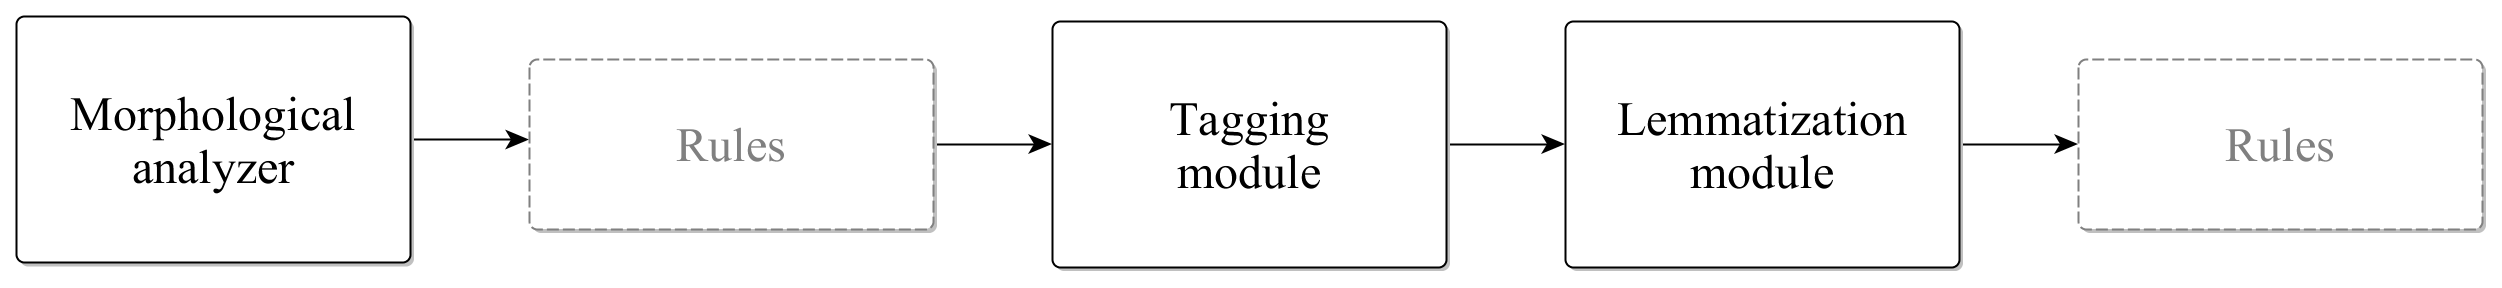
\includegraphics[width=1\textwidth]{MorphTagging/architecture.png} 
  \caption{The architecture of the proposed method}
  \label{fig:purepos-arch}
\end{figure}

In the following, we present its components making the morphological tagging effective. 
In that way,  underlying statistical models are introduced first, then we show how symbolic algorithms are incorporated. 

\subsubsection{The PoS tagging model}

\begin{figure}[H]
  \centering
  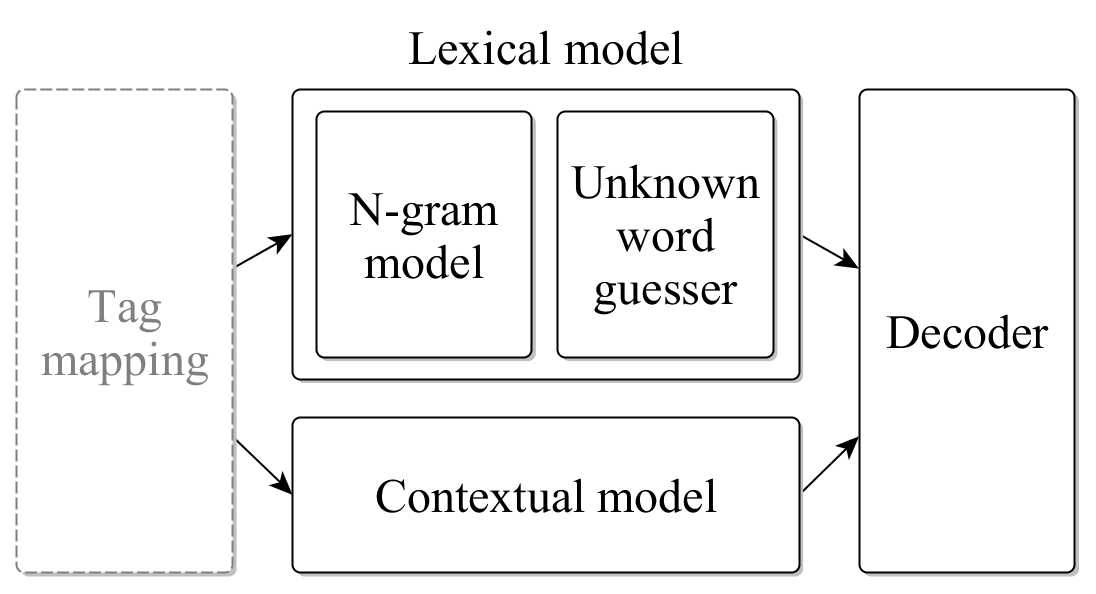
\includegraphics[width=0.5\textwidth]{MorphTagging/pos_arch.png} 
  \caption{Part-of-speech tagging in the proposed system}
  \label{fig:pos_arch}
\end{figure}

PurePos builds on \acrshort{hmm}-based methods \cite{Rabiner1989,Samuelsson1993} introduced in TnT \cite{Brants2000} and HunPos \cite{Halacsy2007}, allowing it to be fast, simple and effective at the same time. 
As its predecessors, our model (see Figure \ref{fig:pos_arch}) selects the best $t_1 \dots t_m$ label sequence for $w_1 \dots w_n$ words by calculating:
\begin{equation}
\argmax_{t_1^m} \prod_{i=1}^m P(t_i | t_{i-1}^{i-n}) P(w_i|t_{i-1}^{i-n})
\end{equation}

Its contextual model is computed with $n$-gram modeling (cf. Equation \ref{eq:purepos-contextual}) employing \gls{mle} (see Equations \ref{eq:purepos-contextual2a} and \ref{eq:purepos-contextual2b})\footnote{Where $N$ denotes the size of the tagset, while $c(x)$ marks the number of $x$ elements in the training data.}. 
Uni-, bi- and trigram estimates are combined with deleted interpolation thus calculating $\lambda_k$ weights as suggested by Brants \cite{Brants2000}. Even though the order of the model is usually set to 3, it is adjustable in practice. 


\begin{equation}\label{eq:purepos-contextual}
P(t_i | t_{i-1}^{i-n}) \approx \sum_{k=0}^{n-1} \lambda_k \hat{P}(t_i|t_{i-1}^{i-k})
\end{equation}

\begin{equation}\label{eq:purepos-contextual2a}
\hat{P}(t_i|t_{i-1}^{i-k}) = \frac{c(t^{i-k}_i)}{c(t_{i-1}^{i-k})} (k>0) 
\end{equation}
\begin{equation}\label{eq:purepos-contextual2b}
\hat{P}(t_i) = \frac{c(t_i)}{N} (k=0)
\end{equation}

Next, the lexical model ($P(w_i|t_{i-1}^{i-n}$) of our method is composed of two components. 
The first one handles tokens previously seen in the training data, while the second guesses labels for unknown words. 
In fact, each subsystem is doubled (as it is in \cite{Brants2000,Halacsy2007}) maintaining separate models for uppercase and lowercase words. 

Handling of previously seen words is carried out approximating $P(w_i | t_{i}^{i-n})$ with word-tag co-occurrences: 
\begin{equation} \label{eq:purepos-lexical}
P(w_i | t_{i}^{i-n}) \approx  \sum_{k=0}^{n-1} \lambda_k \hat{P}(w_i|t_{i}^{i-k})
\end{equation}

\label{sec:purepos-guesser}
$\hat{P}(w_i|t_{i}^{i-k})$ is calculated with \acrlong{mle}, while deleted interpolation is applied with $\lambda_k$ weights. 
As in the contextual model, $k$ is set to 2 in applications.

As regards tagging of unknown words, we use -- in accordance with Brants -- the distribution of rare\footnote{Rare words are considered to be those that occur less than 10 times in the training data.}
tokens’ tags for estimating their \gls{pos} label. 
Since suffixes are strong predictors for tags in agglutinative languages, we use their ($\{s_{n-l+1} \dots s_n\}$) $l$ long combined frequencies:

\begin{align}
 P(t|s_{n-l+1}, \dots, l_n) 
 \approx \frac{ \hat{P}(t|s_{n-l+1}, \dots, s_n) + \theta_i \hat{P}(t|s_{n-l}, \dots, s_n)}{1+\theta_i}
\end{align}

In doing so, $\theta_i$ parameters are calculated applying successive abstraction, while \gls{mle} is utilized  again for computing $\hat{P}(t|s_{n-l+1}, \dots, s_n)$. 

Concerning decoding, beam search is utilized, since it can yield multiple tagging sequences at the same time. 
In that way, the tool is also able to produce tagging scores of sentences \eqref{eq:purepos-score} allowing us to incorporate further components using partly disambiguated word sequences. 

\begin{equation}\label{eq:purepos-score} %%TODO: ez történik, kell ez ide?
Score(w_1^m,t_1^m) = \log \prod_{i=1}^m P(w_i|t_i,t_{i-1})P(t_i|t_{i-1},t_{i-2})P(l_i|t_i,w_i)
\end{equation}

\subsubsection{The lemmatization model}

\begin{figure}[H]
  \centering
  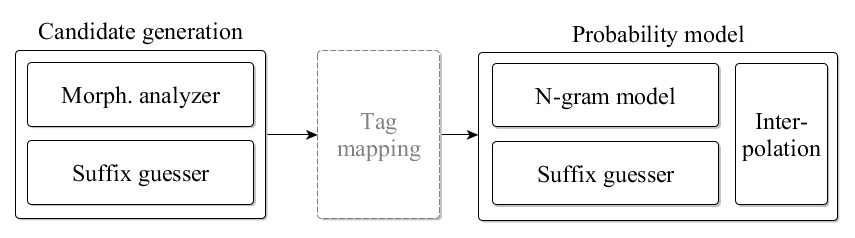
\includegraphics[width=0.8\textwidth]{MorphTagging/lemma_arch.png} 
  \caption{The data flow of the lemmatization component}
  \label{fig:lemma-arch}
\end{figure}

Lemmatization is performed in two steps (cf. Figure \ref{fig:lemma-arch}). 
First, candidates are generated for \emph{(word, morphosyntactic tag)} pairs. 
If morphological analyses are available for the current word, their lemmata are used as candidates, otherwise suffix-based guessing is carried out. 
For this, the guesser (described in Section \ref{sec:purepos-guesser}) was extended to handle lemma transformations as well. 
In doing so, combined labels can represent both the morphosyntactic tag and suffix-transformations for lemmata (for an example see Table \ref{tab:lemma-example}).


\begin{table}[H]
\centering
\caption{Examples for the combined representation of the tag and lemma}
\label{tab:lemma-example}
\begin{tabular}{l | l l}
   \textbf{Word} &  \emph{házam} `my houses’ &  \emph{baglyot} `owl’ \\
   \textbf{Tag} &  \textsc{n.1}s\textsc{pos} &  \textsc{n.acc} \\
   \textbf{Lemma} &  \emph{ház} `house’ &  \emph{bagoly} `owl’ \\
   \textbf{Transformation} & -2+$\varnothing$ &  -4+\emph{oly} \\
   \textbf{Combined label} & (\textsc{n.1}s\textsc{pos}, -2,--) &  (\textsc{n.acc}, -4, \emph{oly}) \\
\end{tabular}
\end{table}


As for picking the right lemma, we utilize a simple scoring model \eqref{lemma-max} that evaluates candidates using their part-of-speech tags:
\begin{equation}\label{lemma-max}
\argmax_l S(l|t,w)
\end{equation}
This method is based on a twofold estimation of $P(l|t,w)$. On the one hand, a unigram lemma model ($P(l)$) calculates conditional probabilities using relative frequency estimates. 
On the other hand, reformulation of $P(l|t,w)$ yields another approximation method:
\begin{equation}\label{lemma-guesser}
P(l|t,w) = \frac{P(l,t|w)}{P(t|w)}
\end{equation}

Substituting this formula to \eqref{lemma-max}, $P(t|w)$ becomes a constant which can be omitted. 
In that way, we can estimate $P(l,t|w)$ employing only the lemma guesser. 
Finally, models are aggregated in a unified ($S$) score: 
\begin{equation}\label{lemma-interpolated}
S(l|w,t) = P(l)^{\lambda_1} P(l,t|w)^{\lambda_2}
\end{equation}


\begin{algorithm*}
\setstretch{1.35}
\begin{algorithmic}[H]
    \ForAll{(word, tag, lemma)} 
        \State candidates $\gets$ generateLemmaCandidates(word, tag)
        \State maxUnigramProb $\gets$ getMaxProb(candidates, word, tag, unigramModel)
        \State maxSuffixProb $\gets$ getMaxProb(candidates, word, tag, suffixModel)
        \State actUnigramProb $\gets$ getProb(word, tag, lemma, unigramModel)
        \State actSuffixProb $\gets$ getProb(word, tag, lemma, suffixModel)
        \State unigramProbDistance $\gets$ maxUnigramProb $-$ actUnigramProb
        \State suffixProbDistance $\gets$ maxSuffixProb $-$ actSuffixProb
        \If {unigramProbDistance $>$ suffixProbDistance}
            \State $\lambda_{2} \gets$ $\lambda_{2}$ $+$ unigramProbDistance $-$ suffixProbDistance
        \Else%If{unigramProbDistance $<$ suffixProbDistance}
            \State $\lambda_{1} \gets$ $\lambda_{1}$ $+$ suffixProbDistance $-$ unigramProbDistance
        \EndIf
    \EndFor
    \State normalize$( \lambda_{1}, \lambda_{2} )$
  \end{algorithmic}
  \caption{Calculating parameters of the lemmatization model}
\label{lemma-interpolation-algorithm}
\end{algorithm*}

The idea of computing $\lambda_{1,2}$ parameters is similar to that seen for the \gls{pos} $n$-gram models. 
However, instead of using positive weights, negative scores are stored for the better model.  
It is calculated iterating over words of the training data (cf. Algorithm \ref{lemma-interpolation-algorithm}):
\begin{enumerate}
  \item first, both components return the best roots for each \emph{(word, tag)} pair, 
  \item then probability estimates for the gold standard lemma are computed,
  \item next, (absolute) error rates of the models are calculated ,
  \item finally, the best model’s weight is decreased\footnote{Since probability estimates are between 0 and 1, decreasing a weight gives higher values.}.
\end{enumerate}
After these steps, $\lambda_k$ parameters are normalized.


\subsubsection{Hybridization}

Although the framework proposed builds on an existing \gls{pos} tagging algorithm, it is extended with a new lemmatization model and is modified to fit agglutinative languages such as Hungarian. 
Hybridization steps listed below show the differences between PurePos and its predecessors \cite{Brants2000,Halacsy2007}.

\begin{description}
  \item[Morphological analyzer] \hfill \\
  First of all, a morphological analyzer is utilized throughout the whole process, therefore probability estimation is performed for valid\footnote{Valid analyses for a word are those which are proposed by the MA.} analyses only.
  \item[Linguistic rules] \hfill \\
  Next, the presented architecture allows rule-based components to modify the analyses of the \acrshort{ma}, in that way, bad candidates can be filtered out. Furthermore, lexical probability scores of analyses can be also given to PurePos, which are then used as context-dependent local distribution functions. 
  \item[Unseen tags] \hfill \\ 
  In contrast to TnT or HunPos, our system is able to handle unseen tags\footnote{Morphosyntactic labels which are not seen in the training data.} properly. On the one hand, if a token has only one analysis not seen before, that one gets selected with 1 lexical probability. Further on, estimation of forthcoming tags are performed using a lower level (unigram) model in this case. On the other hand, the system can also calculate lexical and contextual scores for any tag previously not seen. This can be performed mapping latter tags to a known ones using regular expressions.\footnote{For a complete example see Section \ref{sec:oldhungarian}.}
  \item[$k$-best output] \hfill \\
  Finally, our method decodes tags using beam search. In doing so, one can generate partly disambiguated sentences being apt for linguistic post-processing. Further on, this facility allows the usage of advanced machine learning techniques resulting in more accurate parsing algorithms.
\end{description}


\subsection{Experiments}

\subsubsection{Tagging general Hungarian}\label{sec:porepos-gen}

First, PurePos is evaluated on Hungarian using the Szeged Corpus\footnote{Version 2.3 is utilized in our experiments, since the \acrshort{ma} employed is only compatible with this corpus variation.}~\cite{Csendes2004} (SZC). 
It contains general texts from seven genres being annotated with detailed (MSD) morphosyntactic tags~\cite{Erjavec2012} and lemmata.
Beside the original corpus, we used a variant which is tagged with the analyses of Humor ~\cite{Proszeky1994,Novak2003,Proszeky2005}. 
In our experiments, both corpora were split in 8:2 ratio for training and testing (as in Table \ref{tab:szeged-corpus}) purposes. 

\begin{table}[H]
\centering
\caption{Dimensions of the corpora used}
\begin{tabular}{l r r r r}
  \hline
  & \multicolumn{2}{c}{MSD tagset} & \multicolumn{2}{c}{Humor tagset} \\
  &  Training set &  Test set &  Training set &  Test set  \\
  \hline
  Tokens &  1,232,384 &  254,880 &  980,225 &  214,123 \\
  Sentences &  68,321 &  13,778 &  56,792 &  14,198 \\
  Distinct tags &  1,032 &  716 &  983 &  656 \\
  \hline
\end{tabular}
\label{tab:szeged-corpus}
\end{table}

As a morphological analyzer is an integral part of our method, we tested the tool with two different modules. 
The first setting utilized the MSD tagged corpus and an analyzer extracted from \texttt{magyarlanc}, while the second one applied Humor on the transcribed corpus.

Evaluation is carried out measuring the overall precision of full annotations (i.e \emph{(morphosyntactic tag, lemma)} pairs). 
For significance tests, we have used the Wilcoxon matched-pairs signed-rank test at the 95\% confidence level dividing the test set into 100 data pairs.
Further on, sentence-based accuracies are also provided in some cases. 
The latter metric is computed by considering a sentence to be correct only when all of its tokens are properly tagged. 

Further on, other morphological tagging tools were also evaluated that are available for Hungarian. 
Firstly, \texttt{magyarlanc}, HuLaPos and Morfette\footnote{Version 3.5 is used.} are compared with PurePos.  
%Next, combination of lemmatization and \gls{pos} tagging tools are investigated. 
Secondly, two-phase architectures have been shown to be prosperous (e.g.~\cite{Agic2013,Erjavec2004}), therefore successful modules being commonly applied are also involved in our experiments. 
Concerning \gls{pos} taggers, we use
\begin{itemize}
  \item the trigram tagging method of HunPos,
  \item averaged perceptron learning and
  \item the maximum entropy framework of the OpenNLP~\cite{Baldridge2002} toolkit.
\end{itemize}

As regards lemmatization tools, CST~\cite{Jongejan} and a baseline (as detailed above) method are employed. 
%The latter one results on roots for \emph{(word, tag)} pairs being the most frequent in the training data. 
Beside these components, tag dictionaries have been prepared for HunPos, since it can employ such resources.  
At this point we simulated a setting, where the tagger is only loaded once.
Therefore, a large lexicon was prepared for the tool.
In that way, analyses of the 100,000 most frequent words of Hungarian were provided to the tagger.\footnote{Frequencies are calculated relying on the results of the Szószablya project~\cite{Halacsy2004}.}.

%TODO: keresztvalidáció
%TODO: baseline lemma + purepos

\begin{table}[H]
 \centering
 \caption{Tagging accuracies of Hungarian taggers on the transcribed Szeged Corpus (annotated with MSD labels)}
\begin{tabular}{l r r r}
  \hline
   & \multirow{2}{*}{PoS tagging} & \multicolumn{2}{c}{Morph. tagging} \\
   & &  Token &  Sentence \\
  \hline
  \texttt{magyarlanc} &  96.50\% &  95.72\% &  54.52\% \\
  Morfette &  96.94\% &  92.24\% &  38.18\% \\
  HuLaPos &  96.90\% &   95.61\% & 54.57\% \\
  PurePos &  \underline{96.99\%} &  \underline{96.27\%} &  \underline{58.06\%} \\
  HunPos + BL &  96.71\% &  92.65\% &  36.06\% \\
  HunPos + CST &  96.71\% &  91.19\% &  35.31\% \\
  Maxent + BL &  95.63\% &  92.21\% &  34.82\% \\
  Maxent + CST &  95.63\% &  90.14\% &  29.70\% \\
  Perceptron + BL &  95.19\% &  91.16\% &  29.42\% \\
  Perceptron + CST &  95.19\% &  89.78\% &  27.91\% \\
  \hline
\end{tabular}
\label{tab:morphtag-orig}
\end{table}


\begin{table}[H]
 \centering
 \caption{Tagging accuracies of Hungarian taggers on the transcribed Szeged Corpus (annotated with Humor labels)}
\begin{tabular}{l r r r}
  \hline
   & \multirow{2}{*}{PoS tagging} & \multicolumn{2}{c}{Morph. tagging} \\
   & &  Token &  Sentence \\
  \hline
  Morfette &  97.60\% &  94.73\% &  51.58\% \\
  HuLaPos &  97.19\% &  95.53\% &   57.55\% \\
  PurePos &  \underline{98.65\%} &  \underline{98.58\%} &  \underline{81.78\%} \\
  HunPos + BL &  97.41\% &  89.93\% &  32.07\% \\
  HunPos + CST &  97.41\% &  94.69\% &  52.40\% \\
  Maxent + BL &  94.81\% &  88.82\% &  28.19\% \\
  Maxent + CST &  94.81\% &  92.33\% &  40.10\% \\
  Perceptron + BL &  95.97\% &  88.85\% &  29.11\% \\
  Perceptron + CST &  95.97\% &  93.32\% &  45.13\% \\
  \hline
\end{tabular}
\label{tab:morphtag-humor}
\end{table}

% % % % % % % % % % % % % % % % % % % % % % % % % % % % % % % % % % % %
First of all, there are notable discrepancies between the results on the two datasets (cf. Tables \ref{tab:morphtag-orig} and \ref{tab:morphtag-humor}). 
On the one hand, performance discrepancies can be explained by the morphological analyzers used.
These tools have different coverage, thus they affect the results of parsing chains built on them.
On the other hand, the two corpora utilize different annotation schemes:
\begin{itemize}
  \item First, the original corpus contains foreign and misspelled words being tagged with a uniform \textsc{x} tag. 
  Due to the various syntactic behavior of such tokens, their labels could not be estimated using their context or their suffix properly.
  \item Further on, date expressions and several named entities are tagged with a single MSD code resulting in lemmata composed of more than one words. (An example is \emph{Golden Eye-oztunk} `we visited the Golden Eye’ being lemmatized as \emph{Golden Eye-ozik} `to visit the Golden Eye’.) 
  Such phenomena could be hard to handle for lemmatizers.
\end{itemize}
These differences can have a huge impact on morphological disambiguation algorithms.
In our case, they decrease the accuracy of MSD-based systems, while allow Humor-based ones to produce better annotation  (since the corresponding corpus is free of such phenomena).

In general, results show that the best-performing systems are PurePos, HuLapos, \texttt{magyarlanc} and Morfette.
Besides, HunPos also achieves high \acrshort{pos} tagging scores, while other two-stage taggers are far behind state-of-the-art results. 
As regards learning methods of the OpenNLP toolkit, their precision indicate that they cannot handle such labeling problems precisely.
Further on, both of the standalone lemmatizer degrade accuracy. 
This reduced performance can be due to their design: the baseline method was not prepared for handling unknown words, while CST was originally created for inflectional languages. 

An explanation for the high morphosyntactic labeling score of PurePos is that it uses morphological analyzers to get analyses candidates. 
This component can reduce the number of unknown words, thus enabling it to provide better annotations.
While HunPos also uses such resources, it can only handle static lexicons which limits its accuracy.
%In that way, the huge number of inflected word-forms could be handled accurately.

As regards \texttt{magyarlanc}, it also yields first-class results (95.72\% precision) on the MSD-tagged corpus, however, its language specific components inhibit its application on other corpora. 
Further on, HuLaPos is an interesting outlier.
It is based on pure stochastic methods, but it can still achieve high precision.
Next, Morfette also provides accurate annotations (concerning \acrshort{pos} labels only), however it has problems with computing the roots of words.

Results show that PurePos provides the most accurate annotations amongst tested tools.
Further on, its advance over other systems is statistically significant (Wilcoxon test of paired samples, p < 0.05)\footnote{Pairwise tests were carried out comparing token-level accuracies of PurePos and other competing tools on each corpus.}.
In addition, sentence-based accuracies (especially on the Humor-tagged corpus) also confirms the superior performance of our method. 
These values reveal that most of the tools result in erroneously tagged sentences in more than half of the cases, while the same number for our method is much less (42\% and 18\% respectively). 

It was shown that the presented algorithm can produce high quality morphosyntactic annotations handling the huge number of inflected forms of Hungarian.
Further on, it can also produce precise root candidates for both previously seen and unseen tokens due to its improved lemma computing method.
In that way, Purepos is a suitable tool for morphological tagging of Hungarian and other agglutinative languages.
%
%Next, comparison of full annotation scores reveals that our lemmatization algorithm significantly outperforms others. 
%Furthermore, its lemmatization method outperforms all other systems available for Hungarian.

\subsubsection{Resource-scarce settings}

Next, PurePos is compared to other taggers on less-resourced scenarios.
For this we use systems\footnote{Unfortunately, we could not measure the performance of \texttt{magyarlanc}, since the current release of the tool cannot be trained.})  and corpora described in Section \ref{sec:porepos-gen}.
For this, the amount of the training data was limited (cf. Table \ref{tab:small-szeged}).
In that way, we draw learning curves of systems, evaluating them on both versions of the test set.

\begin{table}[H]
\centering
\caption{The number of tokens and sentences used for training the taggers}
\label{tab:small-szeged}
\begin{tabular}{ r | r r r r r}
Sentences & 2,000 & 4,000 & 6,000 & 8,000 & 10,000 \\
Tokens (MSD-tagged corpus) & 13,555 & 26,496 & 53,563 & 79,916 & 107,113 \\
Tokens (Humor-tagged corpus) & 20,863 & 41,740 & 82, 964 & 121,026 & 146,816 \\
\end{tabular}
\end{table}


\begin{figure}[H]
  \centering
  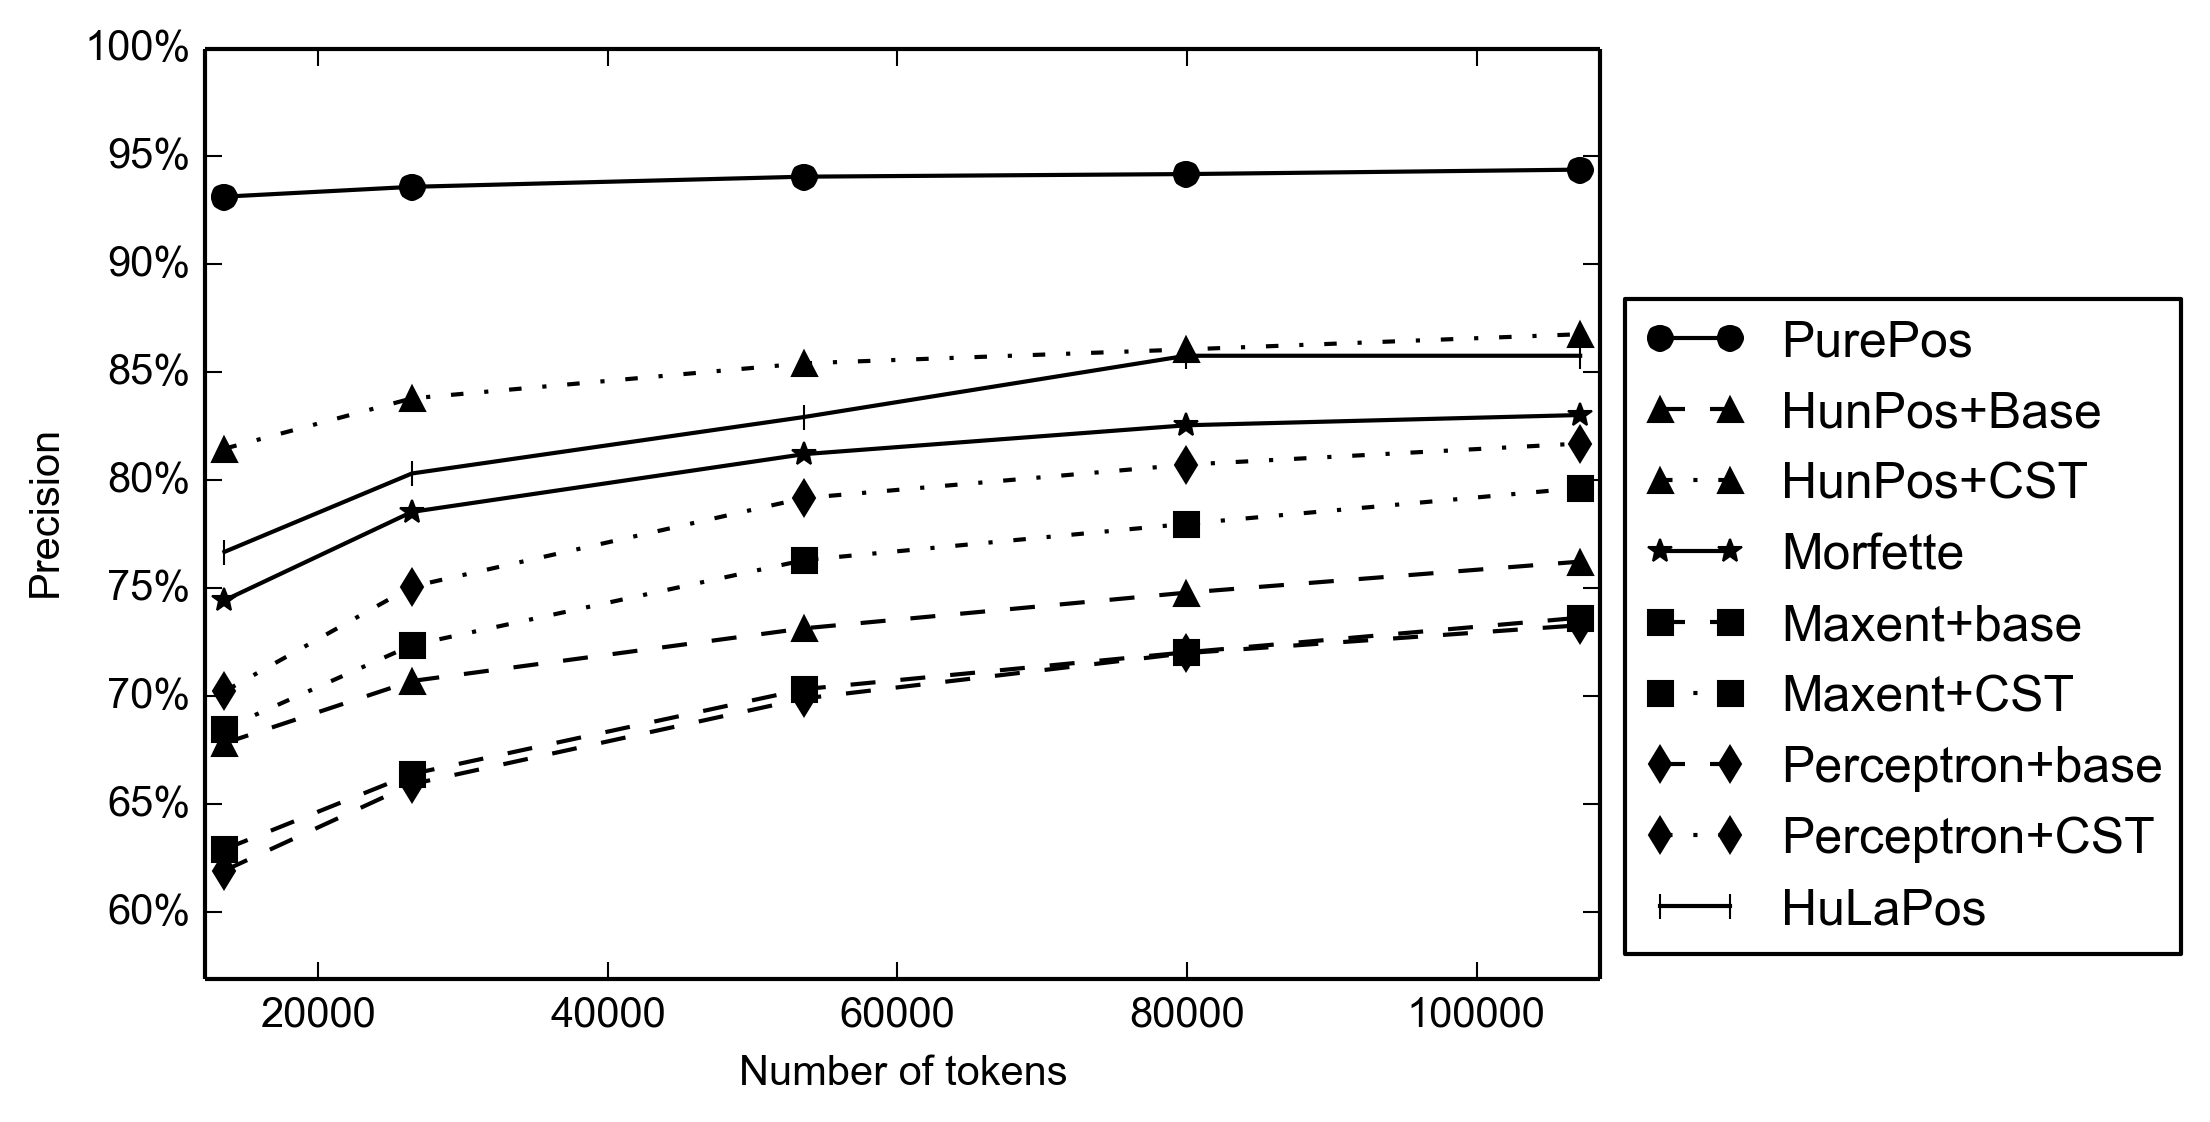
\includegraphics[width=1\textwidth]{MorphTagging/msd_token.png} 
  \caption{Learning curves (regarding token accuracy) of full morphological taggers on the Szeged Corpus (using MSD labels)}
  \label{fig:msd-token}
\end{figure}

\begin{figure}[H]
  \centering
  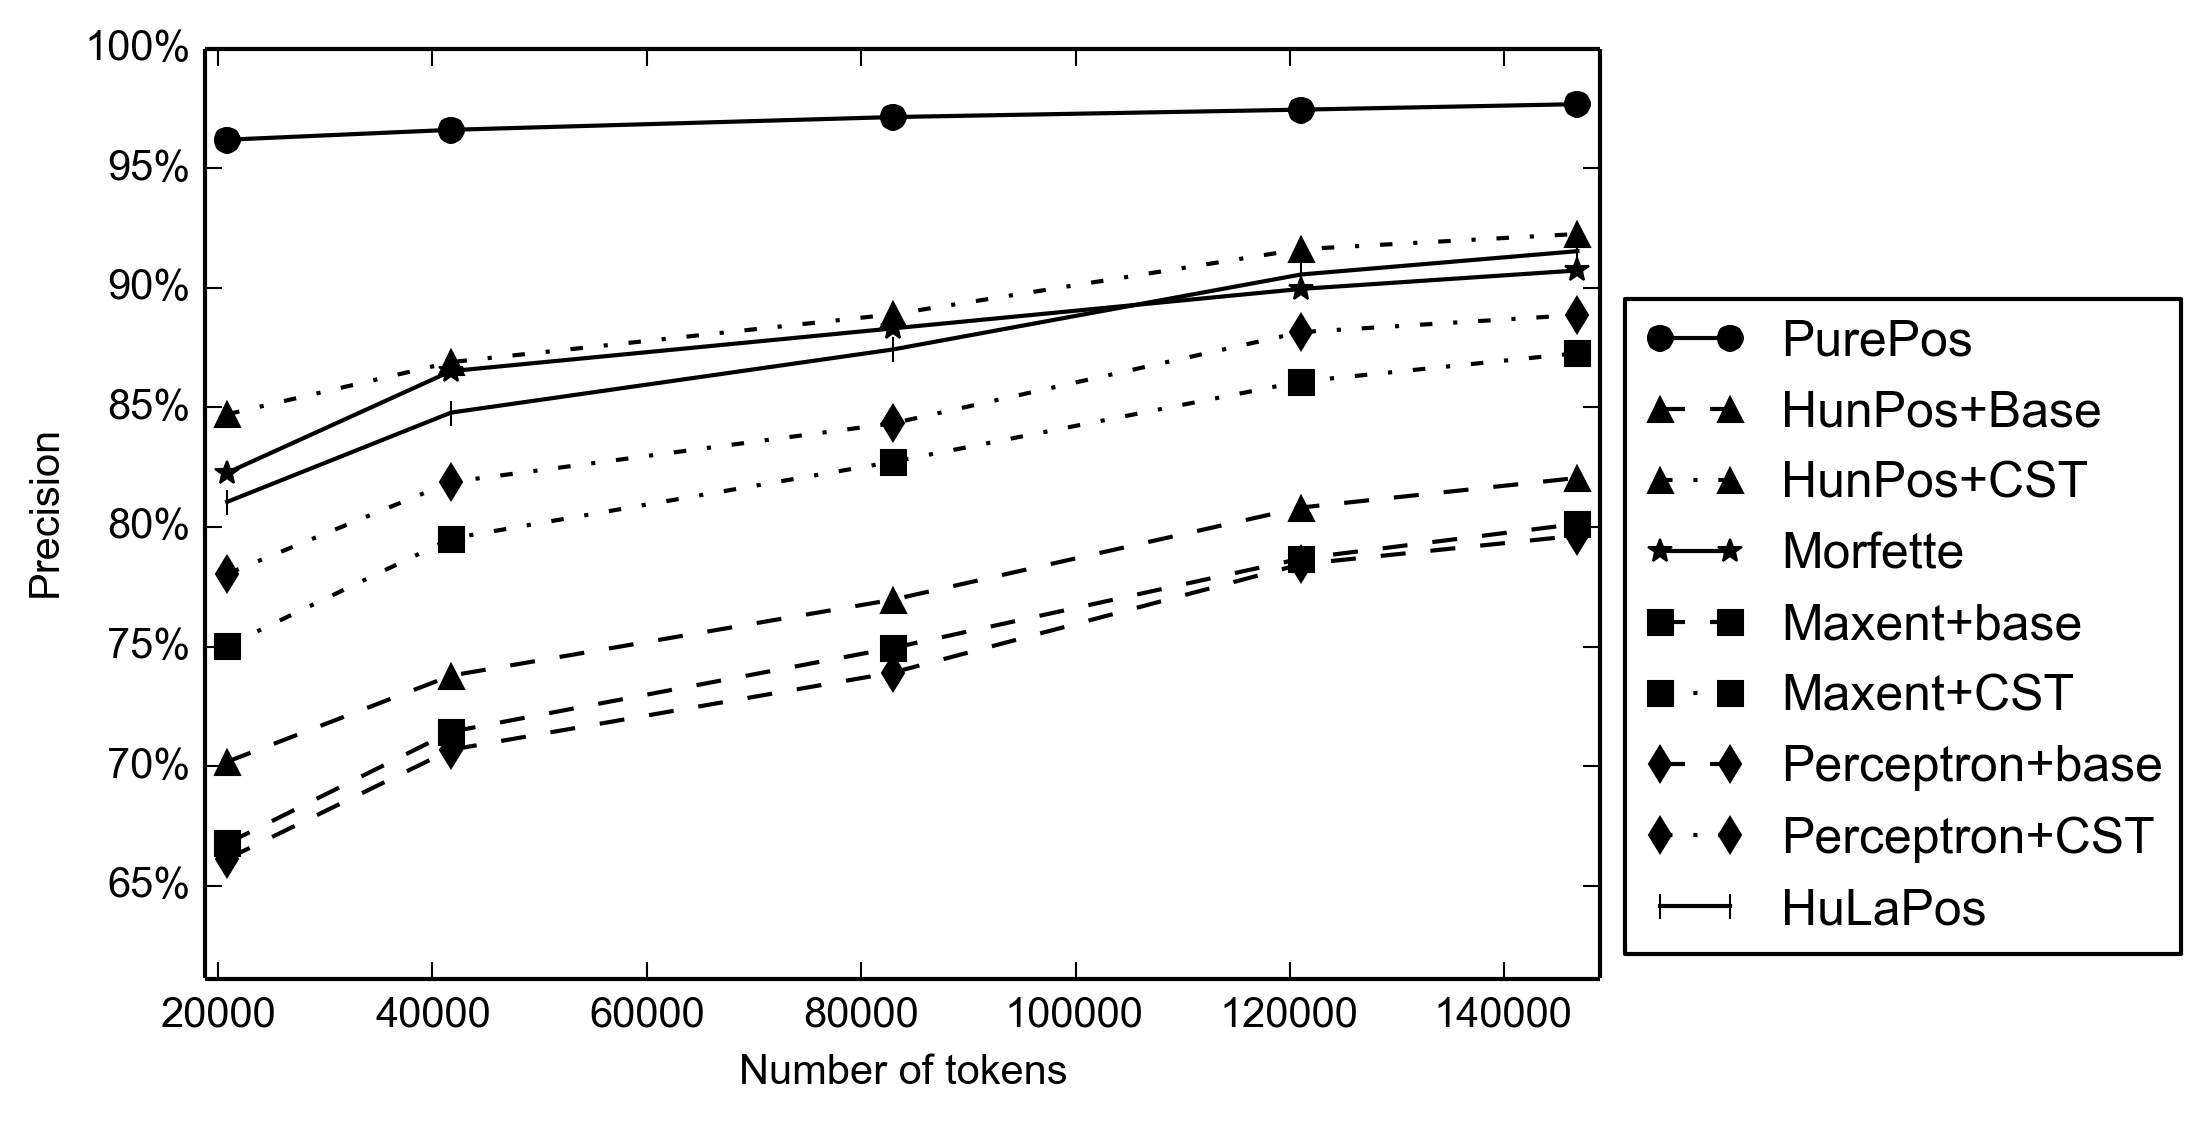
\includegraphics[width=1\textwidth]{MorphTagging/humor_token.png}
  \caption{Learning curves (regarding token accuracy) of full morphological taggers on the Szeged Corpus (using Humor labels)}
  \label{fig:humor-token}
\end{figure}

\begin{figure}[H]
  \centering
  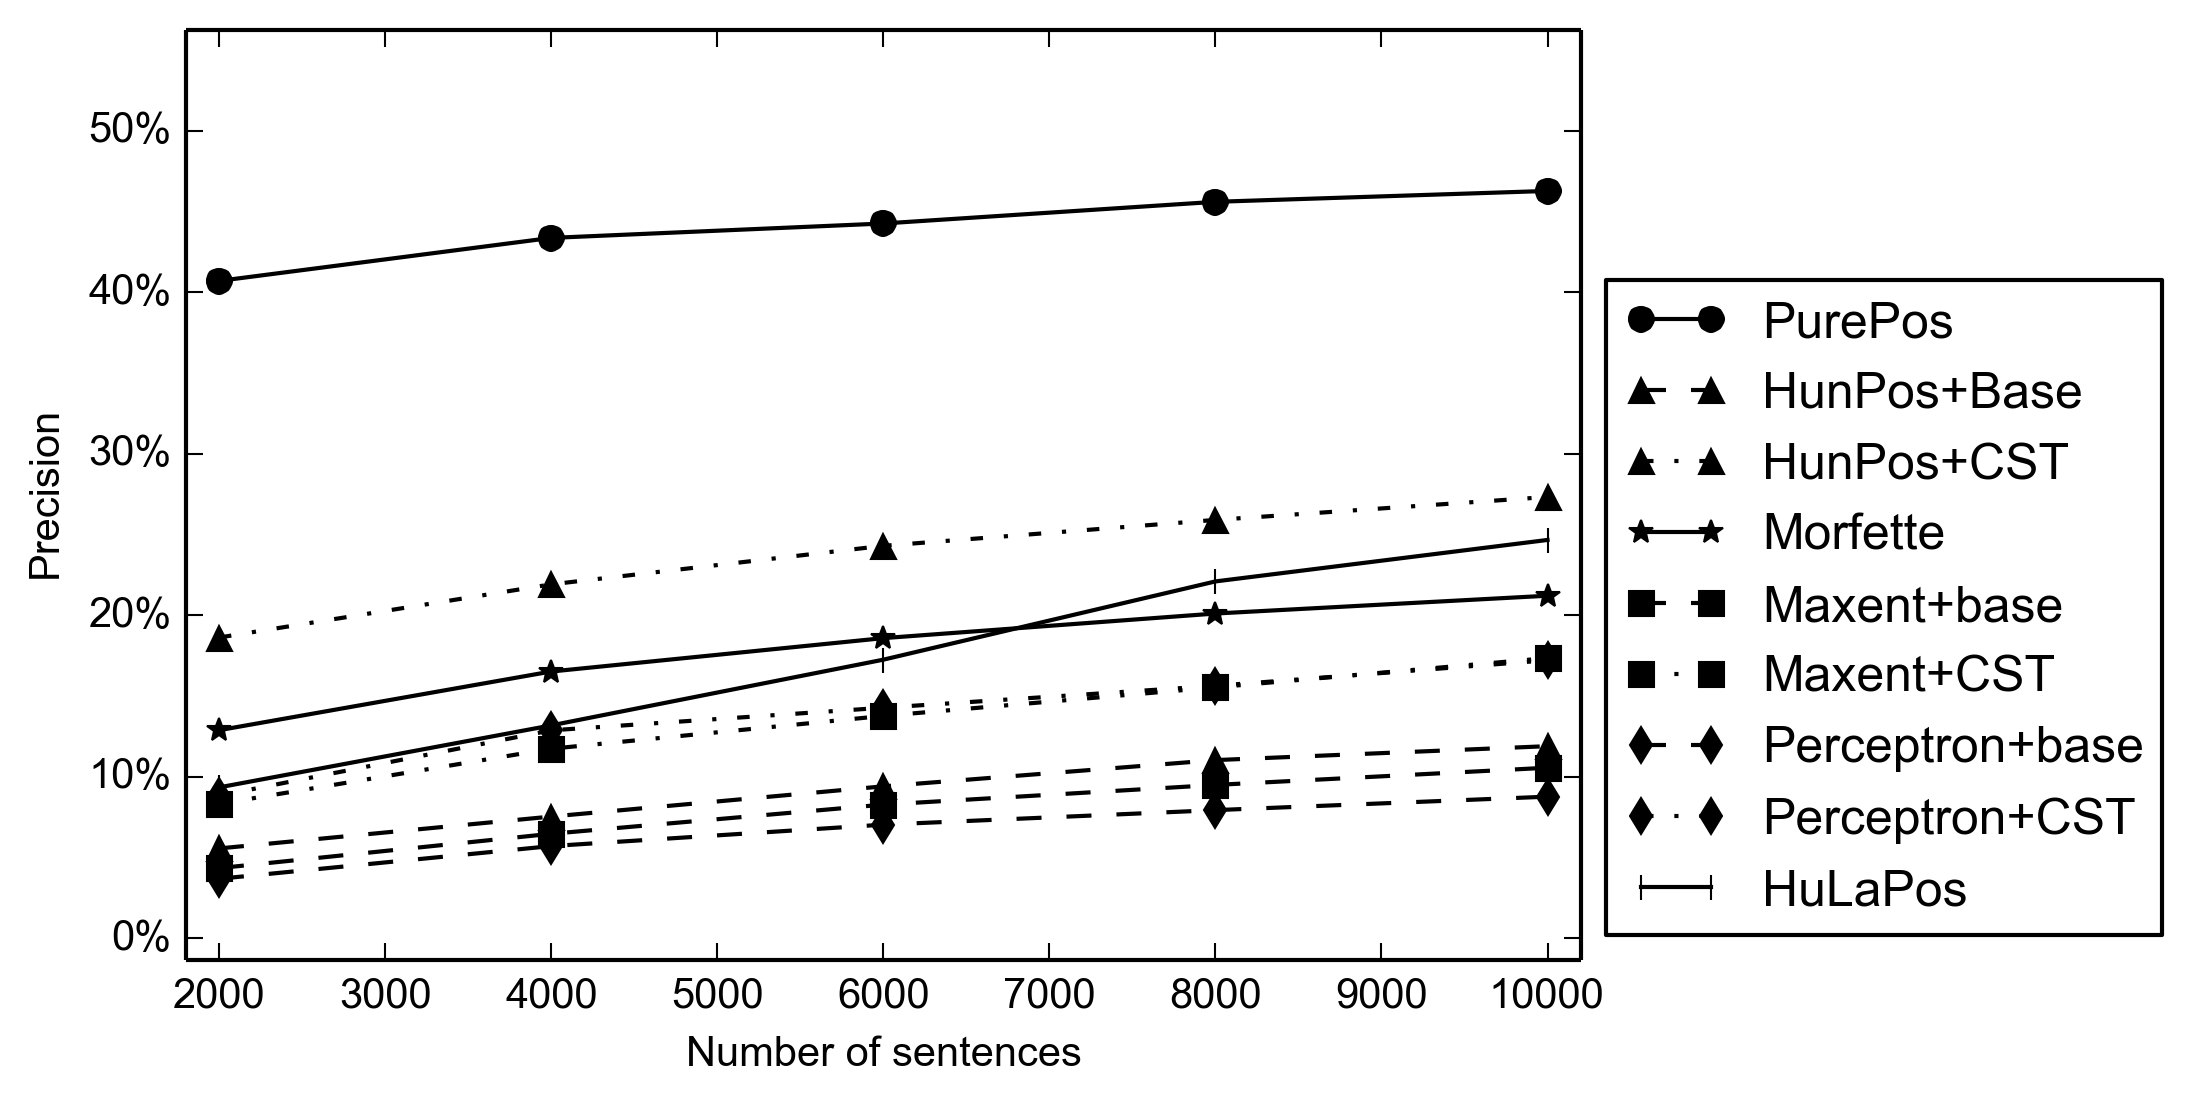
\includegraphics[width=1\textwidth]{MorphTagging/msd_sent.png} 
  \caption{Learning curves (regarding sentence accuracy) of full morphological taggers on the Szeged Corpus (using MSD labels)}
  \label{fig:msd-sent}
\end{figure}

\begin{figure}[H]
  \centering
  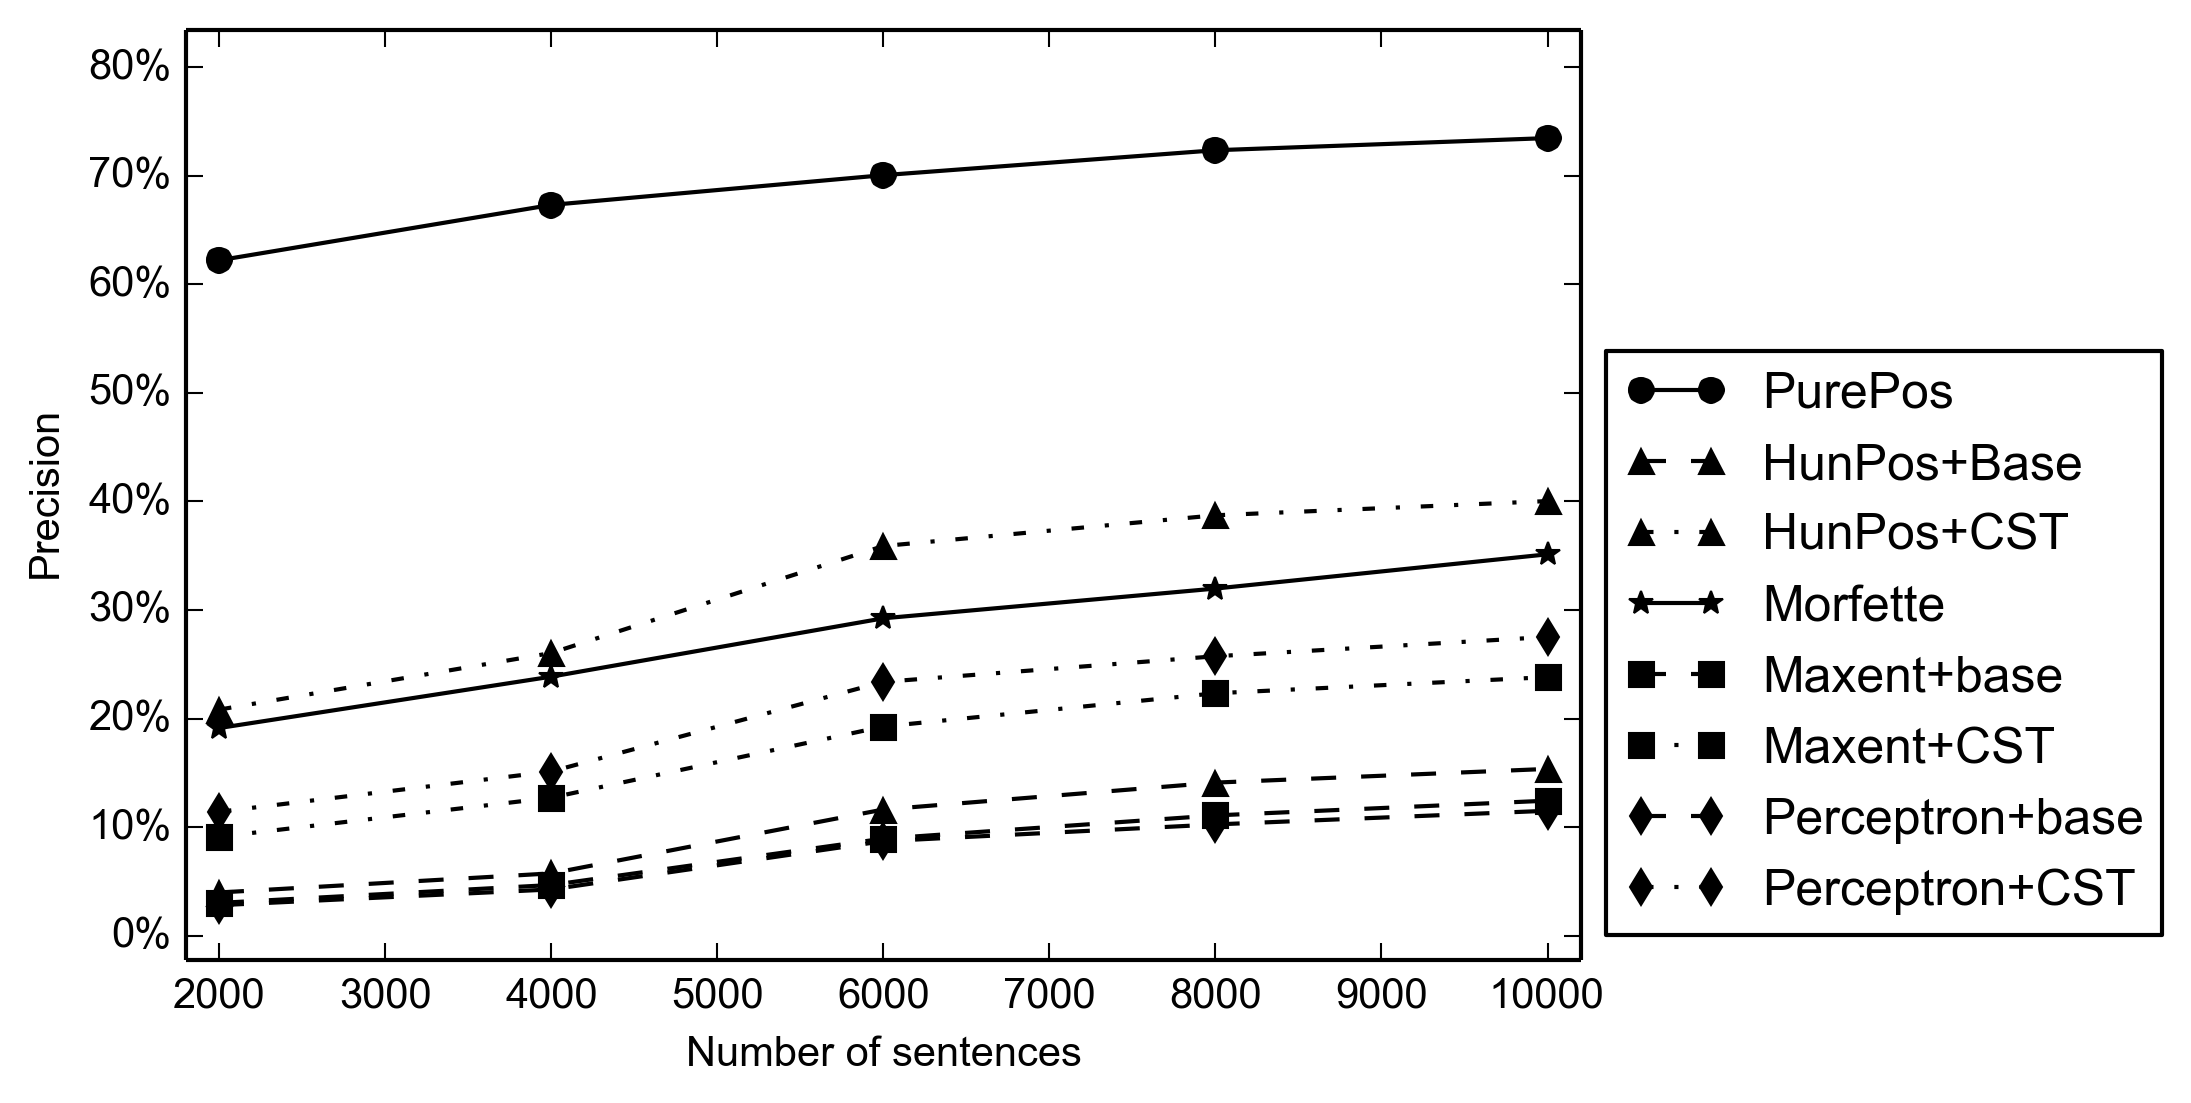
\includegraphics[width=1\textwidth]{MorphTagging/humor_sent.png}
  \caption{Learning curves (regarding sentence accuracy) of full morphological taggers on the Szeged Corpus (using Humor labels)}
  \label{fig:humor-sent}
\end{figure}

First, Figures \ref{fig:msd-token} and \ref{fig:humor-token} present morphological tagging accuracies of systems depending on the number of tokens in the training corpus. 
These results are in accordance with conclusions of our previous experiments, however the differences revealed are higher. 
Further on, the large distance between the precision scores of PurePos and other tools confirms the effectiveness of our  hybrid approach in less-resourced scenarios.


Further on, if we compare (cf. Figures \ref{fig:msd-sent} and \ref{fig:humor-sent}) the taggers' sentence-based precisions, the gap between their performance are much more emphasized. 
For example, having only 2,000 sentences for training (with MSD tags) the proposed algorithm results in 40.71\% sentence precision compared to the second best of 18.62\%.

In brief, we have shown that the architecture of PurePos allows producing accurate annotations when the amount of training data is limited. Therefore, our method could be used for morphological tagging scenarios of agglutinative languages when there is just a few thousand manually annotated sentences are available.

\subsubsection{The case of Middle- Old-Hungarian}
\label{sec:oldhungarian}

Next, we present a tagging task showing the effectiveness of all the hybrid components available in PurePos. 
In a project~\cite{NovakOMK,Novak2013} aiming at the creation of an annotated corpus of Middle Hungarian texts, an adapted version of the Hungarian Humor morphological analyzer \cite{NovakOMK} was used\footnote{The adaptation of Humor and the annotation are the work of Attila Novák and Nóra Wenszky. The author's contribution is the enhancement of the morphological tagging chain.}. 
This tool was originally made to annotate contemporary Hungarian, but the grammar and lexicon were modified to handle morphological constructions existed in Middle Hungarian but have since disappeared from the language. 
In the experiments described here, we used a manually disambiguated portion of this corpus. The data was labeled using a rich variant of the Humor tagset having cardinality over a thousand.

\begin{table}[H]
\centering
\caption{Characteristics of the used corpus}\label{tab:oldhun-corpus}
\begin{tabular}{l r r r}
\hline
& Training & Dev. & Test \\
\hline
Documents & 140 & 20 & 30 \\
Clauses & 12,355 & 2,731 & 2,484 \\
Tokens & 59,926 & 12,656 &  11,763\\
\hline
\end{tabular}
\end{table}

The corpus is split into three parts (see Table \ref{tab:oldhun-corpus}) for the experiments. 
The tagger was trained on the biggest one, adaptation methods were developed on a separate development subcorpus, while final evaluation was done on the test set.
We used precision as an evaluation metric, but unambiguous punctuation tokens were \emph{not} taken into account (in contrast to how taggers are evaluated in general). 
They are ignored because the corpus contains a relatively large amount of punctuation markers which would distort the comparison.
Methods were evaluated twofold: full morphological disambiguation accuracies were calculated for tokens and they were also computed to obtain clause-level precision values. 
In addition, \gls{err} \eqref{eq:err} is calculated measuring the percentage of mistakes ($E$) of a baseline tagger ($b$) that are corrected by an enhanced method ($n$). 

\begin{equation}\label{eq:err}
\err(b,n) = \frac{E(b)-E(n)}{E(b)}
\end{equation}

We used the improved trigram-based algorithm derived from HunPos and implemented in PurePos (PP) as a baseline \gls{pos} tagger. 
This basic chain is enhanced step-by-step investigating the impact of each component.
First, the \acrshort{ma} and the new lemmatization method is analyzed on the development set (cf. Table \ref{tab:oldhun-baselines}). 

\begin{table}[H]
\centering
\caption{Baseline disambiguation accuracies on the development set}\label{tab:oldhun-baselines}
\begin{tabular}{l r r r}
\hline
 & Tokens & Clauses \\
\hline
% PP+BL & 93.20\% & 88.99\% & 55.58\% \\
PP+BL  & 88.99\% & 55.58\% \\
% PP+SL & 93.20\% & 89.01\% & 51.78\% \\
% PPM+BL & 97.77\% & 97.22\% & 84.85\% \\
PPM+BL  & 97.22\% & 84.85\% \\
% PPM+SL & 97.77\% & 97.50\% & 85.98\% \\
PP + CL & 92.14\% & 65.40\% \\
PPM + CL & 97.58\% & 86.48\% \\
\hline
\end{tabular}
\end{table}


On the one hand, we compare the \gls{pos} tagging method of PurePos with (PPM) and without the morphological analyzer (PP).
On the other hand the simple unigram-based (BL) lemmatizer (cf. Section \ref{sec:purepos-guesser}) is evaluated against the proposed one (CL). 
First, it was found that the usage of a morphological component is indispensable. 
Next, results show that the proposed algorithm yields a significant error rate reduction compared to the baseline. 
This improvement is even more notable  (28.42\% \acrshort{err}) when a dedicated morphological analyzer is not used.

In the next, several experiments are presented to exhaust hybrid facilities of PurePos, thus yielding a more accurate tagger. 
To that end, the development set was utilized to analyze common error types and to develop hypotheses.

\paragraph{Mapping of tags}

In contrast to other Hungarian annotation projects, the tagset of the historical corpus distinguishes verb forms that have a verbal prefix from those that do not, because this is a distinction important for researchers interested in syntax.\footnote{Hungarian verbal prefixes or particles behave similarly to separable verbal prefixes in most Germanic languages: they usually form a single orthographic word with the verb they modify, however, they are separated in certain syntactic constructions.} 
This practically doubles the number of verb tags\footnote{320 different verb tags occur in the corpus excluding verb prefix vs. no verb prefix distinction. This is just a fraction of the theoretically possible tags.}, which results in data sparseness problems for the tagger. 
In the case of a never encountered label having a verbal prefix marking, one can calculate probability estimates for that tag by mapping it to one without a verbal prefix. 
This solution is viable, since the distribution of prefixed and non-prefixed verbs largely overlap. 
Applying this enhancement (TM), we could increase notably the accuracy of the system on the development set (to 86.53\% clause level precision).

\paragraph{Preprocessing}

Another point of improvement is to filter analyses of Humor (FI). 
Exploiting the development set, a preprocessing script was set up which has five simple rules. 
Three of them catches the tagging of frequent phrases such as \emph{az a} `that' in which \emph{az} must be a pronoun. 
Further on, two domain specific lexicons were employed to correct the erroneous annotation of proper names that coincide with frequent common nouns or adjectives. 
Using these correction rules the overall performance on the development set was further raised to 86.77\% clause accuracy.


%%%%%%%%%%%%%%%%%%%%%%%%%%%%%%%%%%%%%%%%%%%%%%%%%%%%%%%%%%%%%%%%%%%%

\paragraph{$k$-best output}
The $k$-best output of the tagger can either be used as a representation to apply upstream grammatical filters to or as candidates for alternative input to higher levels of processing. 
Five-best output for our test corpus has yielded an upper limit for attainable clause accuracy of 94.32\% (on the development set). 
%These can either be used as a representation to apply upstream grammatical filters to or as candidates for alternative input to higher levels of processing.
While it is not directly comparable with the ones above, this feature could e.g. be used by syntactic parsers.


\begin{table}[H]
\centering
\caption{Disambiguation accuracies of the hybrid tool on the test set}
\label{tab:oldhun-test}
\begin{tabular}{l r r r}
\hline
 & Full & Clauses  \\
\hline
Baseline  & 89.47\% & 55.07\% \\
PurePos  & 96.48\% & 80.95\% \\
\hspace{0.2cm} + TM  & 96.51\% & 81.17\% \\
\hspace{0.2cm} + FI  & 96.60\% & 81.55\% \\
\hspace{0.2cm} + all  & 96.63\% & 81.77\% \\
\hspace{0.2cm} + all with \emph{k}-best  & 98.66\% & 92.30\% \\
\hline
\end{tabular}
\end{table}
 
Enhancements are validated evaluating them on the test set.
Data in Table \ref{tab:oldhun-test} shows that each linguistic component improves the overall chain significantly\footnote{We used the Wilcoxon matched-pairs signed-rank test at p < 0.05}.
Further on, using the $5$-best output sequence of the tagger provides us much more golden annotations. 
These are available for 92.30\% of the clauses and for 98.66\% of the tokens.

Therefore, we have shown that one can further increase the tagging accuracy by employing hybrid facilities of PurePos. 
%In this section, linguistic knowledge has been used to raise the overall accuracy.
First, rules were employed filtering our erroneous analyses candidates, then unseen tags were mapped to previously seen ones successfully. 
Finally, we have shown that the 5-best output contain significantly more golden annotations.





% \pagebreak

\section{Combination of morphological taggers}\label{sec:combination}
Although high accuracy tagging tools are generally available, sometimes their performance is not satisfactory and shall be increased further.
In cases where very high annotation quality is required, variance of tools should be considered.
Disparate methods can result in different sorts of errors, therefore their combination can yield better algorithms.
Even though this idea is not new, being present in both machine learning and \acrshort{nlp} literature, there has not been much work done on in this field for morphologically rich languages. 

In this section, the case of agglutinative languages is investigated by experimenting with Hungarian morphological disambiguator tools.
First, we give a brief overview about \acrshort{pos} tagger combination methods.
Next, discrepancies of two taggers are presented allowing us to create a new combination architecture.
Finally, we evaluate the proposed method by measuring its improvement over baseline tools used.

\subsection{Background}

The design process of a combined tagger system involves several steps\footnote{Statements are based on studies of Brill and Wu~\cite{Brill1998} and Halteren et al.~\cite{Halteren2001}.}.
First, it needs to be examined whether the errors of components are different enough to outperform the best individual system significantly.
Then an appropriate combining scheme must be found.
Decisions to be made by a combination algorithm can be of at least two sorts: 
\begin{enumerate}
  \item it can either always select the output of one of the bottom-level systems, or 
  \item it can generate an output of its own that may differ from the output of each individual embedded system. 
\end{enumerate}

When applying the former solution, errors of embedded systems determine a theoretical upper limit on the accuracy of the combined system, since it can never generate the expected output whenever neither of the embedded classifiers generate it.
Thus, the latter solution seems more beneficial in theory.
However, the complexity of the annotation task to be performed and the available training data may have an influence on which of these options is feasible and how they perform in practice.
E.g. if the cardinality of the output annotation and features involved in training is high, there may be either data sparseness or performance problems with the second option.

As regards combination strategies, a basic method is majority voting.
Other, more advanced, schemes involve training a top-level classifier based on the individual embedded systems.
This class of schemes is commonly referred to as stacking learners.
The top-level classifier may use various features of both the inputs and the outputs of the bottom-level classifiers when making its decision. 

One of the first attempts of combining English PoS taggers was presented by Brill and Wu \cite{Brill1998}.
They propose memory-based learning which employs contextual and lexical clues.
In their experiments, the solution where the top-level learner always selects the output of one of the embedded taggers outperformed the more general scheme that allowed the output differ from either of the proposed tags.
Next, a comprehensive study by van Halteren et al. \cite{Halteren2001} details an overview of previous combination attempts.
Further on, the authors show that cross-validation can be used to train top-level classifiers for an optimal utilization of the corpus.
They found a scheme performing best characterized as generalized voting.
Although it can yield annotation differing from the output of the embedded taggers, it can also be interpreted as a stacking method.
However, the cardinality of the tag set and the dimensionality of the feature space were modest compared to that of our case.

A system of different architecture is presented by Hajič et al. \cite{Hajic2001}: in contrast to the parallel and hierarchical architecture of the systems above, it employs a serial combination of annotators starting with a rule-based morphological analyzer, followed by constraint-based filters feeding statistical taggers at the end of the chain. 

We use metalearners with cross-validation, since such schemes \cite{Brill1998,Halteren2001} perform effectively.
Further on, language-specific symbolic components are utilized as well, as they can help to handle the rich morphology of the target language.
%In that way, we improve existing methods. 
First, the underlying architecture of general combination methods is modified to produce lemmata candidates as well.
Then, features investigated which fit the best for agglutinative languages.

\subsection{Discrepancies of taggers}

Evaluating taggers on general Hungarian can show that two of the best performing tools (our new method and HuLaPos) significantly diverge by the errors they made.
In our evaluation scheme, a detailed analysis of errors was carried out first, aiming to reveal their possible combined performance.
For this, we utilized the Humor-tagged Szeged Corpus (described in \ref{sec:porepos-gen}).
We kept the training sentences (80\% of the corpus), but the rest was split into two parts. The first half was employed for development purposes, while the second one was set apart for the final evaluation (cf. Table \ref{tab:comb-data}).

\begin{table}[H]
\centering
\caption{Number of sentences and tokens used for training, tuning and evaluating combination algorithms}\label{tab:comb-data}
\begin{tabular}{l r r}
\hline
& Tokens & Sentences \\
\hline
Training set & 980,225 & 56,792\\
Development set & 105,779 & 7,099 \\
Test set & 108,344 & 7,099 \\
\hline
\end{tabular}
\end{table}

First of all, we could not compare word class error rates one-by-one to reveal differences of taggers, since the cardinality of the tagset is over 1,000.
Further on, we could neither rely on Brill's well-known formula (cf. \cite{Brill1998}), as it gives hard-to-interpret unlimited negative values when there is a considerable amount of overlap between the errors investigated.
Therefore, a new metric, called Own Error Rate ($\oer$), was introduced to measure the relatedness of the taggers' errors.
We used the formula 
\begin{equation}
\oer(A,B)=\frac{\text{\#errors of }A\text{ only}}{\text{\#errors of either }A\text{ or }B}
\end{equation}
for calculating the percentage of tagger $A$ being wrong but $B$ being correct in proportion of all errors made by either $A$ or $B$.

\begin{table}[H]
\centering
\caption{Error analysis of PurePos and HuLaPos on the development set}\label{tab:comb-disambig-comp}
\begin{tabular}{l r r r}
\hline
& Tagging & Lemmatization & Full disambig. \\
\hline
% \hline
% Disagreement rate& 2.40\% & 1.98\% & 3.08\% \\
Agreement rate & 97.60\% & 98.02\% & 96.92\% \\
%Agr on not correct/One mistags & 22.09\% & 7.10\% & 18.26\% \\
They are right when they agree & 99.30\% & 99.85\% & 99.29\% \\
%%Agreement on erroneous annotation & 0.70\% & 0.15\% & 0.61\% \\
One is right when they disagree & 97.53\% & 98.89\% & 97.14\% \\
%\hline
$\oer($PP, HL$)$ & 22.41\% & 11.66\% & 21.16\% \\
$\oer($HLP, PP$)$ & 53.58\% & 80.21\% & 58.24\% \\
\hline
\end{tabular}
\end{table}

To begin, we investigated the agreement of tools on the development set.
As Table \ref{tab:comb-disambig-comp} shows:
\begin{enumerate}
 \item they agree on the full annotation in most of the cases,
 \item matching tags and lemmata are almost always right, 
 \item one of them (frequently) knows the correct annotation even when their guesses do not match.
\end{enumerate}

Secondly, own error rates indicate that even though HuLaPos performs worse than PurePos, the errors are fairly balanced between them. 

\begin{table}[H]
\centering
\caption{Precision of the oracle and baseline systems on the development set}\label{tab:comb-disambig-acc}
\begin{tabular}{l r r r}
\hline
& Tagging & Lemmatization & Full disambig. \\
\hline
PurePos & 98.57\% & 99.58\% & 98.43\% \\
HuLaPos & 97.61\% & 98.11\% & 97.03\% \\
Oracle & 99.26\% & 99.83\% & 99.22\% \\
\hline
\end{tabular}
\end{table}

Finally, the theoretical maximum performance of the combination (marked as oracle) is presented in Table \ref{tab:comb-disambig-acc}.
Assuming a hypothetical oracle always selecting the correct \emph{(tag, lemma)} pairs from the tools' suggestions, the accuracy of the better tagger can be further increased eliminating 72.73\% of PurePos' errors. 

\subsection{Improving PurePos with HuLaPos}

To utilize combination through cross-validation, the training set was split into 5 equal-sized parts.
Level-0 taggers (PurePos and HuLaPos) were trained 5 times using the 4/5 of the corpus while the rest of the sentences were annotated by both taggers in each round.
The union of these automatically annotated parts were used to train the (level-1) metalearners.
Furthermore, this technique allowed us to utilize all the training data in each level, yet separating the two phases of the training process. 

Concerning the question of choosing a level-1 learner we followed Witten et al. \cite{Witten2011} for investigating only ``relatively global, smooth'' algorithms.
We utilized \footnote{C4.5 decision tree algorithm was involved in our experiments, but it was unable to handle the large amount of feature data used.} the naïve Bayes (NB) classifier \cite{John1995} and instance-based (IB) learners \cite{Aha1991}.
The latter in addition to be simple, had been previously shown to perform well in similar combination tasks.
Another important decision was to apply metalearners only in cases of disagreement, since the tools’ agreement rate was high.

There are at least two parameters which must be set for IB learners.
First, a distance function needs to be selected, then the number of neighborhooding events has to be restricted.
In that way, we opted on using Manhattan distance and decided to rely only on the single closest item. 

Moving on, Hungarian has a tagset with a cardinality of over a thousand and an almost unlimited vocabulary, which would make the tag-picking approach inviable. Therefore, we applied methods choosing the tagger but not the tag. 

As regards features, we relied on the set proposed by Brill and Wu \cite{Brill1998}, since it had been shown (cf. \cite{Halteren2001}) to be simple but powerful. It (FS1 in Table \ref{tab:comb-feature-sets}) consists of several lexical properties such as
\begin{enumerate}
 \item the word to be tagged, 
 \item immediate neighbours of the token,
 \item tags suggested for the corresponding word,
 \item tags suggested for neighbouring tokens.
\end{enumerate}

\begin{table}[H]
\centering
\caption{Feature sets used in the combination experiments}\label{tab:comb-feature-sets}
\begin{tabular}{l l l}
\hline
Feature set & Base FS & Additional features \\
\hline
FS1 & Brill-Wu & --- \\
FS2 & FS1 & whether the word contains a full stop or hyphen \\
FS3 & FS1 & use at most 5-character suffixes instead of the word form \\
FS4 & FS2, FS3 & --- \\ 
FS5 & FS1 & guessed tags for the second word both to the right and left \\
FS6 & FS4 & use at most 10-character suffixes instead of the word form \\
\hline
\end{tabular}
\end{table}

First, we examined how these attributes can be extended systematically (see Table \ref{tab:comb-feature-sets}) to fit languages with a productive morphology.
Since wordforms in Hungarian are composed of a lemma and numerous affixes, longer suffixes features are utilized to handle data sparseness issues.
Further on, wider context were also employed to manage the free word order nature of the language. 


Performing the experiments, we used the WEKA machine learning toolkit \cite{Hall2009}.
Improvements were measured on \acrshort{pos} tagging, lemmatization, as well as on the full annotation scenario.

\begin{table}[H]
\centering
\caption{Error rate reduction of combination algorithms on the development set. IB is the instance based learning algorithm, while NB denotes naïve Bayes.}\label{tab:comb-reduction-rates}
\begin{tabular}{l r r r r r r}
\hline
Task:& \multicolumn{2}{c}{Tagging} & \multicolumn{2}{c}{Lemmatization} & \multicolumn{2}{c}{Full annotation} \\
\hline
Feature set & \multicolumn{1}{l}{NB} & \multicolumn{1}{l}{IB} & \multicolumn{1}{l}{NB} & \multicolumn{1}{l}{IB} & \multicolumn{1}{l}{NB} & \multicolumn{1}{l}{IB} \\
\hline
FS1 & 19.03\% & 24.65\% & -6.21\% & 22.24\% & 5.06\% & 22.89\% \\
FS2 & 18.91\% & 24.82\% & -0.80\% & 23.85\% & 4.95\% & 23.16\% \\
FS3 & 21.04\% & 27.60\% & 0.80\% & 26.65\% & 18.42\% & 25.31\% \\
FS4 & 20.92\% & \underline{27.90\%} & 4.01\% & 26.65\% & 18.96\% & 25.20\% \\
FS5 & 16.37\% & 17.55\% & -19.24\% & 16.03\% & -0.70\% & 18.47\% \\
FS6 & 19.27\% & 27.30\% & -17.03\% & \underline{26.85\%} & 16.16\% & \underline{25.79\%} \\
\hline
\end{tabular}
\end{table}


Table \ref{tab:comb-reduction-rates} shows \acrlong{err} scores of different systems compared to PurePos. 
These results reveal that naïve Bayes classifier (NB) performs significantly worse than instance-based learners (IB) even when using seemingly independent features.
Further on, lemma combination turned out to be an insoluble task for that classifier.
Improvements show that word shape features (FS2) always help on tagging, while increased contexts (FS5) are not as powerful.
An interesting outcome of combining \acrshort{pos} taggers was that the word to be tagged was not necessary amongst the features (see FS4 and FS6 at Table \ref{tab:comb-reduction-rates}).
However, utilization of longer suffixes boosts the performance.
In addition, they are also beneficial in cases where lemmatization is part of the task. 

Now we turn on experiments yielding the best combination architecture for full morphological annotation.

\subsubsection{Combination of morphological taggers}

A simple combination structure is to treat annotations as atomic units letting the metalearner choose the output of one of the baselines (cf. Figure \ref{fig:comb1}).
Results on the development set suggest utilizing instance-based methods with the FS6 feature set for this architecture (cf. ``Full annotation'' column in Table \ref{tab:comb-reduction-rates}). 

\begin{figure}[H]
  \centering
  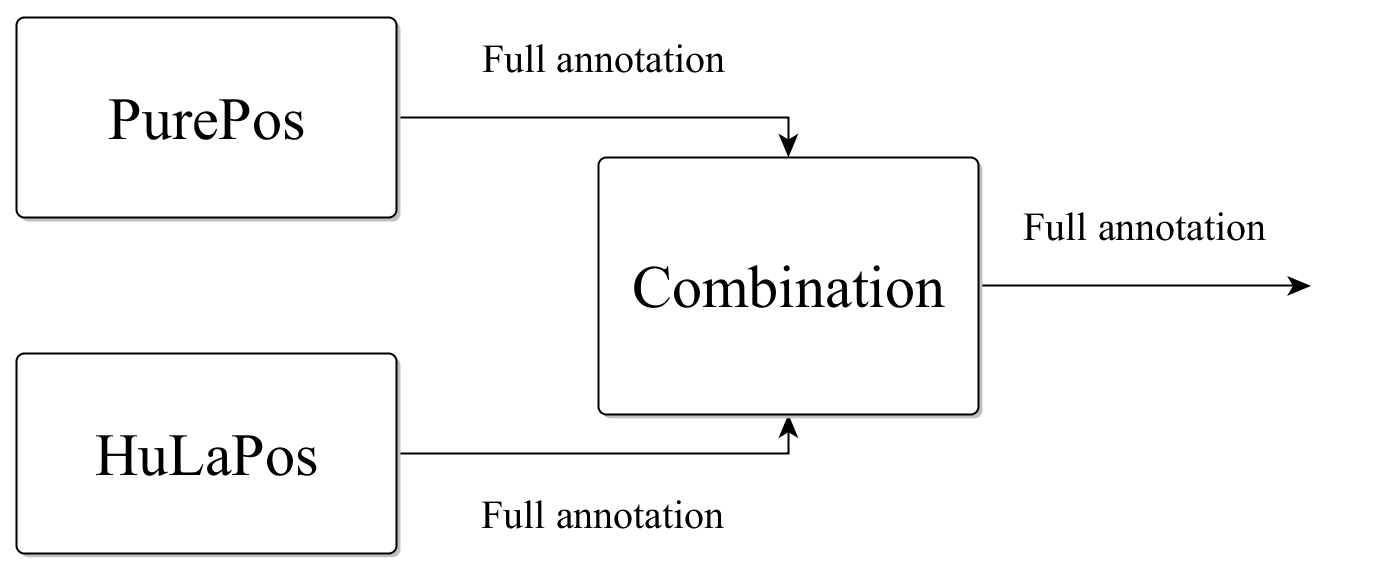
\includegraphics[scale=0.2]{MorphTagging/comb1.png} 
  \caption{Combining the output of two morphological taggers}
  \label{fig:comb1}
\end{figure}

\subsubsection{Combining PoS taggers only}

Another plausible scheme is to combine only the \acrshort{pos} tagger modules of the tools (see Figure \ref{fig:comb2}).
However, in doing so, one has to deal with lemmatization as well.
A straightforward solution for this to employ the lemmatizer of the better annotator tool (PurePos).
Following this, the best tag selection model could be constructed (cf.
Table \ref{tab:comb-reduction-rates}) using IB learning with FS4 features.

\begin{figure}[H]
  \centering
  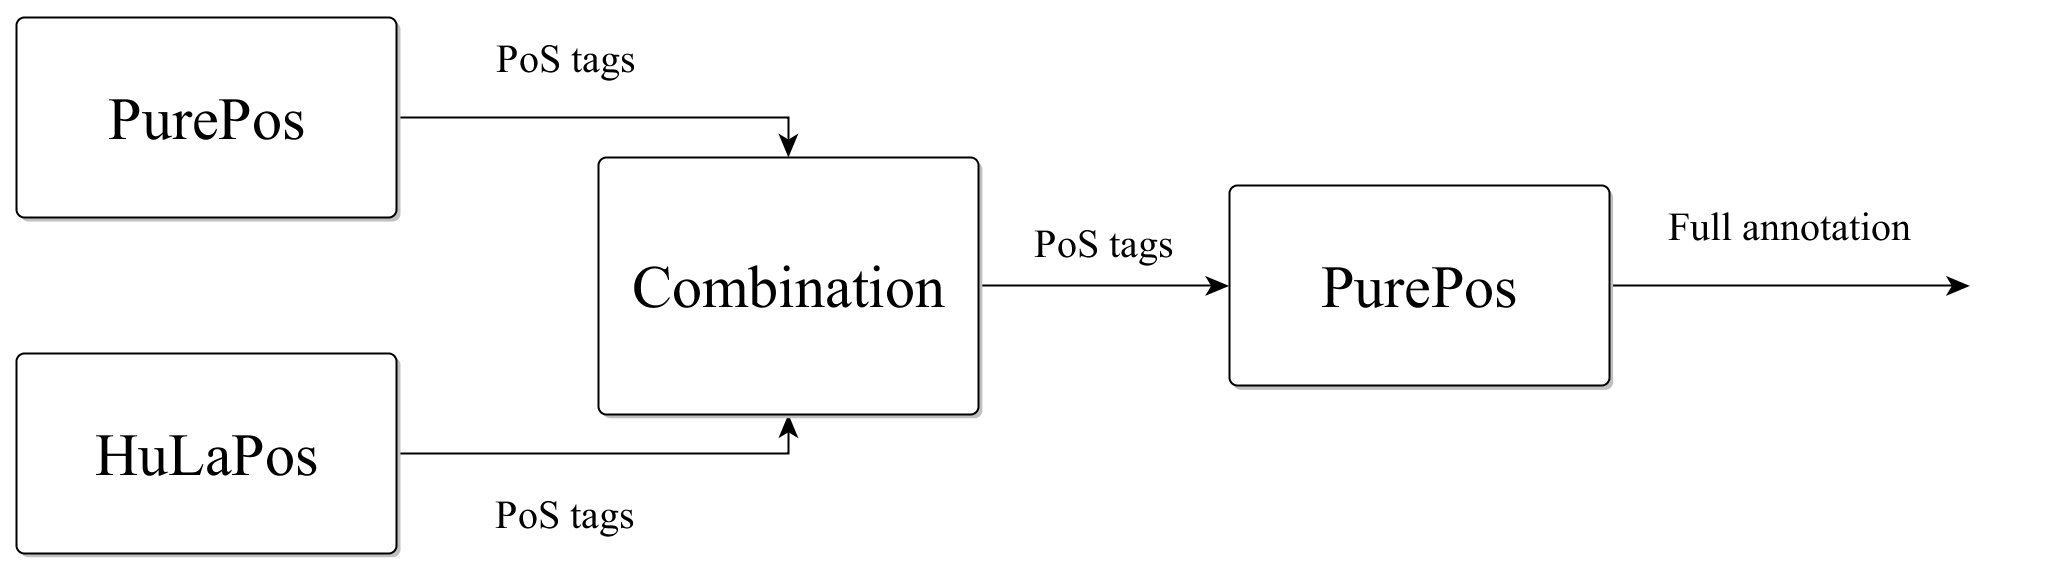
\includegraphics[scale=0.2]{MorphTagging/comb2.png} 
  \caption{Combining the output of two PoS taggers and using also a lemmatizer}
  \label{fig:comb2}
\end{figure}

Although this algorithm allows us to create a better morpho-syntactic tagger compared to that of above, the gain in lemmatization remains much lower (6.81\%).
Consequently, the overall accuracy improvement measured in the development set (25.26\%) is inferior.

\subsubsection{Multiple metalearners}

Finally, the best results are produced using two level-1 learners: one of them chooses the better lemmatizer while the other selects the optimal \acrshort{pos} tagger (cf. Figure \ref{fig:comb3}).
In that  way, this architecture can incorporate the best lemma and tag candidates (as in Table \ref{tab:comb-reduction-rates}) yielding superior performance.
However, a drawback of this configuration that it may result in incompatible tag-lemma pairs\footnote{A lemma and a tag for a word is incompatible if the \acrshort{ma} can analyze the word, but no analysis contains both the lemma and the morpho-syntactic label.}.
To overcome this problem, this combination scheme is enhanced with the Humor morphological analyzer.
This component is used to discover and fix incompatibilities.
With this enhancement, we achieved  32.42\% of improvement on the development set.

\begin{figure}[H]
  \centering
  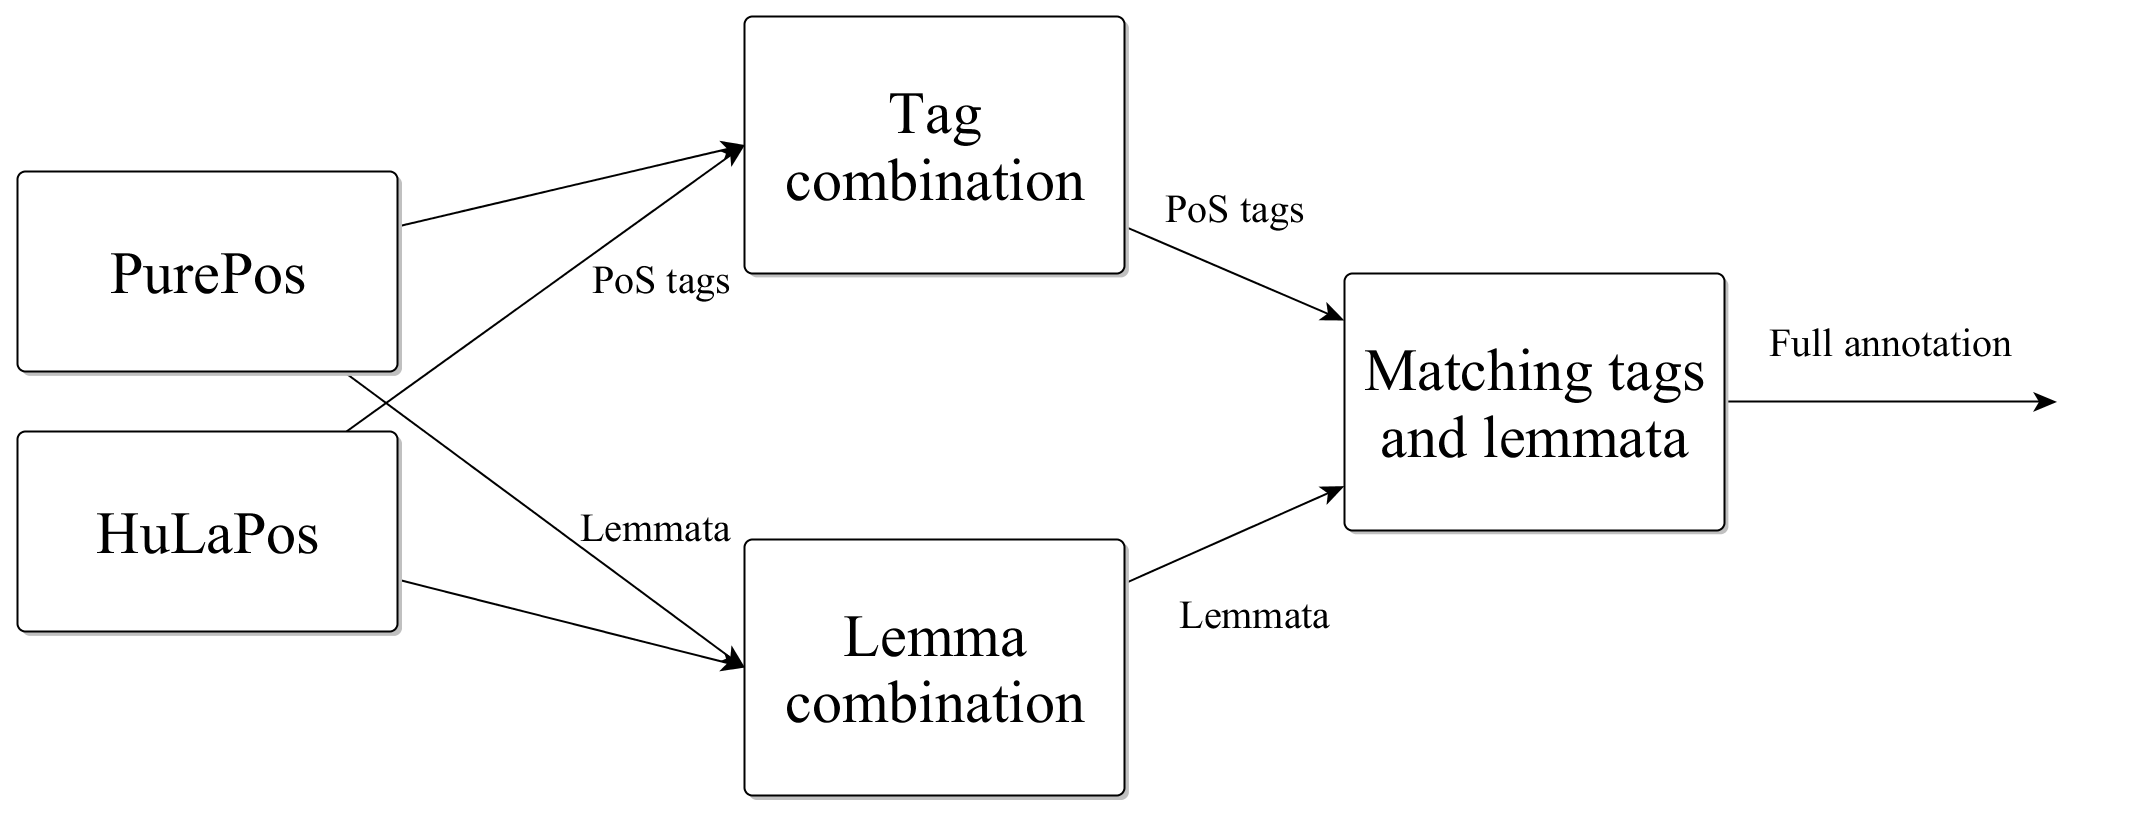
\includegraphics[scale=0.2]{MorphTagging/comb3.png} 
  \caption{Combining the output of two PoS taggers and lemmatizers}
  \label{fig:comb3}
\end{figure}

\subsection{Evaluation}

%In order to validate our hypothesis, stating that the last configuration performs the best, improvements
%Combination schemes presented are evaluated on the unseen test set. %, confirming the results presented above.

\begin{table}[H]
\centering
\caption{Relative error rate reduction on the test set compared to PurePos}\label{tab:comb-eval}
\begin{tabular}{l r r r}
\hline
System & Tagging & Lemmatization & Full disamb. \\
\hline
\textit{Oracle} & 48.60\% & 59.42\% & 51.53\% \\
Disamb. combination & 23.23\% & 23.55\% & 26.86\% \\
Tagger combination & 22.76\% & 13.77\% & 23.81\% \\
Multiple metalearners & 25.07\% & 29.89\% & \underline{28.90\%} \\
\hline
\end{tabular}
\end{table}

All the presented combination schemes are evaluated on the unseen test set. %, confirming the results presented above.
Results show (cf. Table \ref{tab:comb-eval}) that the hybrid architecture using a morphological analyzer achieved the best performance.
While other schemes could also increase the accuracy of PurePos, it resulted in the best tagging precision (98.90\%) of fixing 28.90\% of the baseline system's errors.
This improvement score also shows that our system could capture more then half of the cases which can be fixed by a hypothetical oracle combinator.
Further on, the proposed method also gives the highest error rate reduction in both \acrshort{pos} tagging and lemmatization.
Concerning statistical significance, both the improvements of the presented schemes and their differences are significant at p < 0.05 (using Wilcoxon test of paired samples).
These results show that our new combination architecture can be used in cases when very high disambiguation accuracy is crucial.
Finally, we also confirmed that PurePos and HuLaPos complement each other well resulting in an improved morphological tagger. 



 

 

 

 


 


\chapter{An application of the tagger: estimating morphosyntactic complexity}\label{chap:mlu}

\section{Motivation}

Do linguists need to spend long hours counting morphemes for measuring morphosyntactic complexity? 
Ever since the first studies, \gls{mlu} plays an important role in language development investigations. 
This metric has been widely used for measuring linguistic productivity of children for almost a hundred years. 
Utterance lengths are usually calculated in morphemes (\acrshort{mlum}) being a time-consuming task. 
Even though CLAN toolkit \cite{MacWhinney1992} can count morphemes in utterances, this feature is only available just for a few languages not containing any agglutinative one. %TODO: Kinga szerint az MLUm nem biztos, hogy usually

This chapter presents\footnote{This study is a joint work with Kinga Jelencsik-Mátyus. 
Manual annotation of the data were performed by both of us, while the morpheme counting principles are her work. 
My contribution is the construction of the tagging chain, its adaptation and the automatization of the MLUm calculation.} 
an automatic method for estimating \acrshort{mlum} for Hungarian transcripts. 
We show that PurePos can be used effectively for aiding linguists in this scenario. 
Our approach adapts this tagging tool (cf. Section \ref{sec:purepos}) yielding the first Hungarian tagger for spoken texts. 
Further on, we describe an \acrshort{mlum} estimation method, which is based on the latter tagger, resulting in high quality output. 

First related studies are summarized, then we present resources used for the research. 
Next, the adaptation steps of PurePos are described and the framework designed is introduced. 
Finally, we show that both the tagger and the estimator methods are accurate enough to replace the labor-intense manual calculation.

\section{Background}

Tagging approaches of spoken languages mainly cover only mainstream ones (such as English, Italian or Spanish) while agglutinative ones are usually neglected. 
One of the pioneers in this field was Eeg-Oloffson \cite{Svartvik1982} using  manually annotated transcripts to train a statistical tagger (for English). 
In contrast, there are others employing and adapting statistics of written language corpora \cite{Mendes2004,Nivre1996,Panunzi2004}.
Besides, building domain-specific rules also lead to satisfactory taggers (e.g. \cite{Moreno2003}),
while combination of such systems with stochastic tools \cite{Bick2012} yields effective algorithms as well. 

These previous studies imply that a proper morphological annotation system aiming to process transcripts must be able to handle the following types of difficulties:
\begin{enumerate}
 \item existence of new morphosyntactic tags which are missing from the tagset of the training data,
 \item occurrence of tokens with non-standard orthography in texts,
 \item the number of words unknown to a statistical tagger are increased compared to written language corpora,
 \item if probability estimates are derived from a written language training corpus, the model of stochastic taggers can become non-representative (e.g. the distribution of \acrshort{pos} tags may significantly differ in written and spoken language).
\end{enumerate}

Ever since the complexity of child language has been measured, several methods have been developed. While manual counting prevailed for decades, automatic counting tools have been sought for in the past years.

Several studies (e.g. \cite{Brown1973}) showed that \acrshort{mlum} indicates language development for normal children, especially at very early stages. 
In contrast, \gls{mluw} was shown to be highly correlating \cite{Hickey1991,Parker2005} with the latter in the case of analytical languages such as English or Irish. 
Therefore, some studies concur that \acrshort{mluw} is a reliable measure as opposed to \acrshort{mlum}, where researchers often need to make ad hoc decisions on what (not) to count \cite{Crystal1974}. 

Crystal also points out \cite{Crystal1974} that computing length in morphemes is a good way to measure morphologically complex languages (see e.g. \cite{Bowerman1973}). 
Hungarian is an agglutinative language, thus this measure can be considered to be a more reliable indicator of language development  than \acrshort{mluw} (similarly to Turkish \cite{saygin2010}). 
Moreover, previous studies investigating language development in Hungarian \cite{Reger1990,Weber2011} also employed \acrshort{mlum} as a metric.

In the case of corpora which follow the CHAT guidelines \cite{macwhinney1991childes}, lengths of utterances (including morpheme counting) can be calculated with the CLAN \cite{MacWhinney1992} toolkit. 
This system is widely used, since it has components performing the necessary preprocessing steps. 
One of its modules is MOR that is a morphological analyzer designed for spoken language corpora. 
A subsequent component is POST, doing the morphological disambiguation. 
Finally, a morpheme counter tool using their output is also available. 
In that way, \acrshort{mlum} is usually calculated in a number of languages applying these tools.
However, they lack rules for Hungarian and many other morphologically complex languages, thus none of them can be used for analyzing such transcripts.

We are not aware of any research investigating the tagging of spoken Hungarian. 
Moreover, there is no study aiming to calculate \acrshort{mlum} for Hungarian transcripts automatically. 
Therefore, we introduce adaptation methods for a general-purpose tagger which is then utilized for counting morphemes resulting in accurate \acrshort{mlum} estimates.

\section{Resources}

There is no Hungarian speech corpus morphosyntactically annotated, therefore we use a contemporary one as a base of our research. 
\gls{hukilc} \cite{Matyus2014} has been compiled predominantly for child language variation studies. 
It contains 62 interviews with 4.5--5.5 year-old kindergarten children from Budapest, recorded in the spring of 2012. 
The interviews are 20--30 minutes long consisting different types of story-telling tasks. 
Its transcription was carried out using the \gls{childes} \cite{macwhinney1991childes} following its guidelines. 
The corpus has about 39,000 utterances with 140,000 words.

In order to develop a proper tagger tool, a small part of the data has been manually annotated. 
As a first step, general tagging principles were established. 
We chose the morphosyntactic labels and lemmata of the Humor analyzer ~\cite{Proszeky1994,Novak2003} to represent morphological analyses. 
Next, an annotation manual was developed for human annotators to guide their work during the morphological disambiguation of the corpus. 
In that way, 6 interviews with about 1,000 utterances were labeled manually. 
This gold standard corpus was split into two sets of equal sizes: a development and a test set (see Table \ref{tab:corpus_size}).


\begin{table} [H]
\centering
\caption{Size of the gold standard corpus}
\label{tab:corpus_size}
\begin{tabular}{ l @{\hspace{0.3cm}} r @{\hspace{0.3cm}} r } 
\hline
& Utterances & Tokens \\
\hline
Development set & 509 & 3,340 \\
Test set & 449 & 2,740 \\
\hline
\end{tabular}
\end{table}



The tagset of the corpus has been created to allow both the investigation of morphosyntactic relations and the representation of phenomena typical to transcripts. 
First of all, a new label was introduced to mark filled pauses. 
Further on, the original annotation scheme of Humor distinguishes interjection and utterance words\footnote{Annotation schemes for Hungarian distinguish utterances and interjection words. An utterance word forms a sentence or an utterance alone by interrupting or managing the communication. In contrast, interjections are either onomatopoeic or used to indicate emotions.},
but there are cases in speech when a word bears with both properties (such as \textit{fúú} `woow’). 
Therefore, a new label was created for annotating such tokens properly. 
Finally, the usage of diminutive is common in child transcripts, thus this property was indicated in labels and corresponding suffixes were omitted from lemmata.

\section{Tagging children transcripts}
\label{sec:tagging}
The morphological tagging algorithm employed is a hybrid one. 
It is composed of a morphological analyzer, a stochastic tagger tool and several domain-specific disambiguation rules as well (cf. Figure \ref{fig:speech-tagger}). 
Since the tagset of Humor was chosen to be used for the annotation, a plausible solution was to employ this analyzer. 
Further on, PurePos was utilized to disambiguate between the morphological annotation candidates. 
We used the Szeged Corpus \cite{Csendes2004} to train the tagger, since it is the only manually annotated resource available for Hungarian. 

\begin{figure}[H]
  \centering
  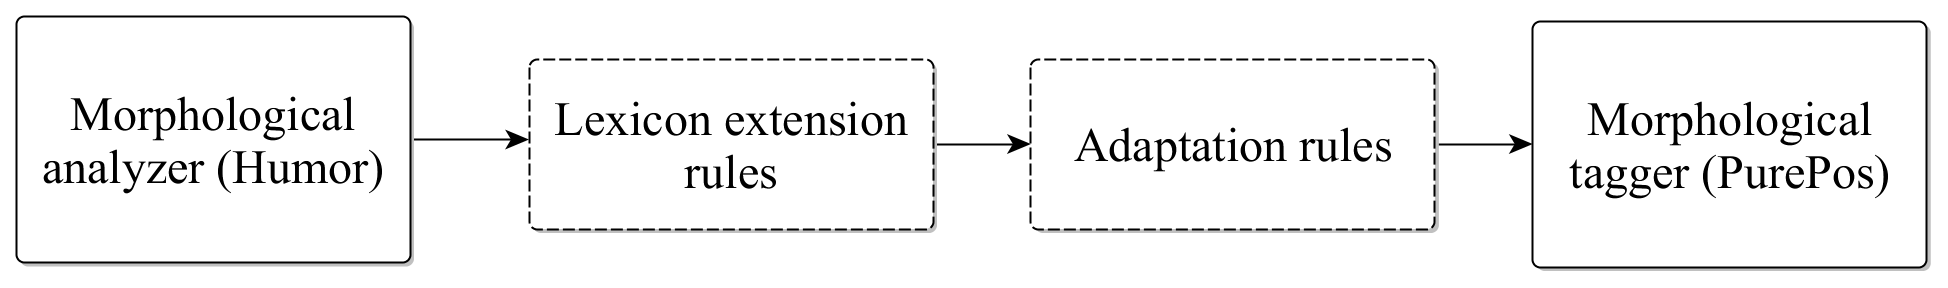
\includegraphics[scale=0.2]{MorphComplexity/mlu_architecture.png} 
  \caption{The architecture of the morphological tagging chain adapted for the HUKILC corpus}
  \label{fig:speech-tagger}
\end{figure}


In order to apply a \acrlong{ma} prepared for written texts, its analyses had to be adjusted for the transcripts. 
Thus, adaptation rules -- based on regular expressions and domain-specific word lists -- were developed.
Their formulation could be done with high confidence, since most of the transcripts contained controlled conversation covering only a few topics. 

As a first step, morphological analyses of about 40 words typical of spoken language were created manually. 
These tokens were mostly interjections not used in written language (such as \textit{hűha} `wow’), while some adverbs were regarded as utterance words in the corpus (e.g. \textit{komolyan} `seriously’). 
Furthermore, those tokens that are written as one word in transcripts but are spelled as two words in formal texts were also added to the lexicon. 
An example is \textit{légyszíves} `please’ which is written formally as \textit{légy szíves}. Finally, diminutive analyses were also provided where it was necessary. 
E.g. \textit{kutyus} `doggy’ was also analysed as \textsc{n.dim} with the lemma \textit{kutya} `dog’ beside the old label \textsc{n} and the \textit{kutyus} `doggy’ root. This process was carried out by investigating the lemmata produced by Humor: if the deletion of the derivational affix resulted in a root enumerated in a domain-specific list, a new diminutive analysis was created as well. 

Concerning the disambiguation process, PurePos was extended with rules to adapt its knowledge to the target domain. 
First, the tagger was forced to assign diminutive analyses when it was possible. 
Then, further enhancements were carried out by investigating the common mistakes of the tool on the development dataset.

A frequent error of the chain was the mistagging of \textit{akkor} `when’ and \textit{azért} `in order to’. 
These words are pronouns and can be categorized as either adverbial, noun phrase level or demonstrative ones, and can also behave as pronomial adjectives. 
Generally, when \textit{akkor} is followed by \textit{amikor} `when’ (as in \textit{Akkor érkezett meg, amikor mentem} `He arrived, when I left’) and when \textit{azért} is followed by \textit{mert} `because’ (as in the sentence \textit{Azért eszik, mert éhes} `He eats, because he is hungry’) these pronouns are demonstrative ones. 
Furthermore, such co-occurances are more common in the transcripts than in the Szeged Corpus, since they are frequently used during reasoning or telling a story. 
As these long-term dependencies could not be learnt by the trigram tagger applied, rules were employed to tag these tokens correctly.

The next issue was the case of the word \textit{utána} `afterwards, then; after him/her/it’. 
It can either be used as an adverb of time (as in the sentence \textit{Utána elindultunk} `Then we left’) and as a postpositional phrase meaning `after him/her/it, following him/her/it’ (as in \textit{Elindultunk utána} `We went after him’). 
The former usage is more frequent in spoken language: when this word is directly followed by conjunctions such as \textit{meg} `and’ or \textit{pedig} `however’, it is always an adverb. 
Therefore, \textit{utána} was tagged as an adverb in the transcripts when it is followed by one of these trigger words. 

The last rule introduced deals with \textit{meg}, which may function as a verbal prefix or as a conjunction.  
Moreover, it is usually an expletive in spoken language.
Therefore, the conjunctive label was assigned to the word when there was not any verb in its two token window.

\section{Computing morphosyntactic complexity}

As a first step, general principles of counting morphemes were established. 
In a language with such a rich derivational system as Hungarian, it is often very complicated to identify the lemmata. 
This is even more difficult in our case, since no common methodology exists to determine the boundary of productivity in child language. 
This was based on studies of Brown \cite{Brown1973}, Retherford \cite{retherford1993guide}, Wéber \cite{Weber2011} and Réger \cite{Reger1990}, with some necessary modifications. 
The basic principles were: 
\begin{enumerate}
 \item only meaningful words were analyzed, thus fillers (filled pauses such as \textit{ööö} `er’), punctuation marks and repetitions are not counted in the utterances;
 \item phatic expressions (e.g. \textit{igen, mhm} `yes, uhm’) serving to maintain communication and not conveying meaning were omitted;
 \item inflectional suffixes and lemmata were each counted as one unit; 
 \item derivational morphemes (including diminutives) were not counted as separate ones,
 \item reciprocal and indefinite pronouns (e.g. \textit{minden\#ki} `everybody’) and compound words (such as \textit{kosár\#labda} `basketball’) were counted as one morpheme.
 \end{enumerate}
 
Following the guidelines of Brown \cite{Brown1973}, proper names (such as \textit{Nagy Béla}, \textit{Sári néni} `Miss Sári’) and lexicalized expressions (e.g. \textit{Jó napot} `Good morning’), which are frequent in speech, were also considered as one unit. 
Their identification was carried out employing rules. 
For this, the method relies on capitalized token sequences and a domain-specific list of words.

As for the automatization of rules, they were implemented using the morphological annotation of the corpus. 
First, each item on the list of fillers was eliminated.
Afterwards, tagged words known to the \acrshort{ma} were split into morphemes by the Humor analyzer. 
If more than one analyses were created for a word, the least complex one was chosen, since analyses only differed in the number of derivative tags and compound markers (which we previously decided not to count) in the majority of the cases.
As the labels of the annotation scheme were composed of morphemic properties, the estimation of unknown words could be based on their tags. 
Therefore, such calculations were carried out counting only the inflection markers in the guessed tags. 

\section{Evaluation}

First of all, morphosyntactic tagging performance of the system was investigated. 
%For this, we calculated precision per token not counting punctuation markers (cf. Section \ref{}).
In that way, full analyses -- containing both the lemmata and the tag -- were compared to the gold standard data, not counting punctuation marks and hesitation fillers.

\begin{table}[H]
\centering
\caption{Evaluation of the improvements on tagging chain}
\label{tab:eval_tag}
\begin{tabular}{ l r r} 
\hline
\multicolumn{1}{l}{\multirow{2}{*}{Morph. tagger}} & \multicolumn{2}{c}{\hspace{0.8cm} Tagging accuracy} \\
& Token &  Sentence \\
\hline
Baseline &  \hspace{0.8cm} 91.97\%  & \hspace{0.8cm} 68.37\% \\
\hspace{0.2cm} + DIM &  94.92\% & 79.96\% \\
\hspace{0.2cm} + CONJ & 95.53\% & 81.74\% \\
The full chain & \underline{96.15\%} & \underline{83.96\%} \\

\hline
\end{tabular}
\end{table}

For measuring the individual advances of the enhancements presented, four different settings were evaluated on the test set. 
The first was a baseline using raw analyses of Humor disambiguated by PurePos. 
The second system (DIM) employed the extended vocabulary and handled the diminutive analyses as described in Section \ref{sec:tagging}. 
The next one -- marked with CONJ -- utilized further rules aiming to tag \textit{azért} and \textit{amikor} correctly. 
Finally, the last system presented contains all the enhancements detailed above.

Measurements in Table \ref{tab:eval_tag} show that the baseline tool tagged erroneously 3 out of 10 sentences. 
On the contrary, each of the enhancements improved the overall performance significantly.
For this, we used the Wilcoxon matched-pairs signed-rank test at p<0.05. 
Furthermore, results indicate that the accuracy of the adapted chain is comparable with that of the tagging methods for written corpora \cite{zsibrata2013magyarlanc}. 

As for the \acrshort{mlu} estimation task, two metrics were used for the evaluation. 
First, \acrlong{mre} was calculated (as in \cite{Witten2011}), comparing the $a_i$ manual morpheme counts with $p_i$ predicted values for the $i$th utterances:
\begin{equation}
MRE = \sum_{i=1}^n \frac{|a_i-p_i|/a_i}{n}
\end{equation}
In that way, this measurement shows the average relative deviation of the estimated morpheme counts from the one of human annotators. 

In addition, Pearson's correlation coefficient\footnote{The notation is the same above, except $\overline{x}$ is the average of $x_i$ values and $n$ denotes the total number of observation.}
 \eqref{eq:corr} (cf. \cite{Witten2011}) was employed as well:
  \begin{gather}\label{eq:corr}
  \frac{S_{PA}}{\sqrt{S_P S_A}} \text{, where } \\
  S_{PA} = \frac{\sum_i{(p_i-\overline{p})(a_i-\overline{a})}}{n-1} \text{, } \nonumber \\
  S_{P} = \frac{\sum_i{(p_i-\overline{p})^2}}{n-1} \text{ and } S_{A} = \frac{\sum_i{(a_i-\overline{a})^2}}{n-1}  \nonumber
  \end{gather}
  indicating the correspondence between the output of the processing chain and the counts of human annotators.


\begin{table}[H]
\centering
\caption{Evaluation of the MLUm estimation algorithm}
\label{tab:eval_est}
\begin{tabular}{ l r r} 
\hline
Tagged utterances & MRE & Correlation \\
\hline
The output of the baseline tool&  0.1325  &  0.9612 \\
The output of the enhanced chain & \underline{0.0449} & \underline{0.9901} \\
Gold standard &  0.0279 &  0.9933 \\
\hline
\end{tabular}
\end{table}

Since both metrics require a gold dataset, morpheme counts have been manually calculated for 300 utterances of the test set.
Table \ref{tab:eval_est} presents the evaluation of the \acrshort{mlum} estimation algorithm on this manually checked corpus. 
First, we evaluated the output of the baseline tagger with our morpheme counter. 
Beside this, both the gold standard data and the output of the enhanced tagging tool were used as an input of the estimator. %enabling a detailed comparison of enhancements presented. 
On the one hand, these results can be interpreted as an in vivo evaluation of the adapted tagger showing significant improvements over the baseline.
On the other hand, it was found that the overall performance of the estimation methodology is outstandingly high.  
The high correlation of the automatic chain indicates that our method can properly measure the morphosyntactic complexity of Hungarian spoken language in practice. 
Therefore, the time-consuming manual counting procedure can be replaced with the proposed method.

\chapter{Methods for a less-resourced domain}\label{chap:clin}

\section{Introduction}

Hospitals produce a huge amount of clinical notes that have been solely used for archiving purposes and have generally been inaccessible to researchers. 
However, application of recent \acrshort{nlp} technology can make accessible the hidden knowledge of archived records, thus boosting medical research. 
While developing text processing tools for medicians is an emerging field in many developed countries, this is not true for less-resourced languages.

To be able to extract information from medical texts, they must be preprocessed properly. 
Firstly, adequate text segmentation methods 
%\footnote{While the term \emph{text segmentation} is widely used for diverse tasks, in our work it denotes the process of dividing text into tokens and sentences.} 
are required for finding token and sentence boundaries. 
Secondly, morphological tagging is an indispensable step for information extraction scenarios. 
Considering the case of Hungarian, there are only a few studies on processing medical records. 
Recently, Siklósi et al. \cite{Siklosi2012,Siklosi2013} have presented a system that is able to correct spelling errors in clinical notes. 
Their system uses a mixture of language models to generate correction candidates, however it focuses only on correctly segmented words. 
Beside error correction, an abbreviation resolution method was also presented by them \cite{Siklosi2013b}, however, problems of text segmentation and  morpho-syntactic tagging are still untouched. 
Furthermore, as far as we know, no study investigates such preprocessing tasks on Hungarian clinical texts. 

Therefore, this chapter presents accurate preprocessing algorithms for noisy medical texts.
Methods were developed and presented for only Hungarian, but they are designed in a way to perform well on other morphologically complex languages as well. 
Firstly, an effective method is introduced for detecting sentence and token boundaries.
The presented system builds on well-known tokenization rules boosting them with the knowledge of a morphological analyzer and the output of an unsupervised filtering algorithm.
Secondly, tagging experiments are presented yielding a viable morphological tagger for Hungarian electronic health records. 
The proposed tool builds on PurePos fixing its most common errors regarding the domain.

\section{Segmenting texts of electronic health records}\label{sec:clin_segm}

Error propagation in a text-processing chain is usually a notable problem, therefore accurate text segmentation methods are essential to process any sort of text properly.
However, notes written by doctors are extremely noisy containing errors which inhibit applications of existing tools.

Even though existing segmentation methods for Hungarian performing well on general domains, they have serious difficulties on clinical texts.
These originate in special properties of the text involving
\begin{inparaenum}[\itshape a\upshape)]
 \item typing errors (i.e. mistyped tokens, nonexistent strings of falsely concatenated words) and
 \item nonstandard usage of Hungarian.
\end{inparaenum}
While errors of the first type can generally be corrected with a rule-based tool, others need advanced methods. 

In this section, a hybrid approach to normalization and segmentation of Hungarian clinical records is presented. 
The method consists of three phases: first, a rule-based clean-up step is performed; then tokens are partially segmented; finally, sentence boundaries are determined. 
We start by detailing the tool's architecture. 
Then, key elements of the sentence boundary detection (SBD) algorithm are described. 
Finally, the system presented is evaluated against a gold standard corpus, and is compared to other tools available.

\subsection{Previous work on text segmentation}

Even though, numerous approaches deal with English noisy texts, only a few attempts have been made (cf. \cite{Siklosi2012,Siklosi2013,Siklosi2013b}) for Hungarian. In addition, the latter studies completely ignores the segmentation problem. What is more, most of the attempt attempts for clinical English also ignores the description of the tokenization/SBD algorithm applied. Therefore, we start with reviewing general segmentation techniques then continue on describing which of them are used successfully for the biomedical domain.

The task of text segmentation is often composed of several subtasks: normalization of noisy text (when necessary), segmentation of words, and sentence boundary detection.  
Although, these subtasks are generally performed one after another, there are approaches (e.g. \cite{zhu2007unified}), where text segmentation and normalization are treated as a unified tagging problem. Further on, handling of abbreviations is often involved during the process, since their identification helps detecting sentence and token boundaries.

As regards tokenization, it is generally treated as a simple engineering problem\footnote{In the case of alphabetic writing systems.} aiming to split punctuation marks from word forms. On the contrary, SBD is a rather researched topic. As Read et al. summarize \cite{read2012sentence}, sentence segmentation approaches fall into three classes: 
\begin{enumerate}
 \item rule-based methods employing domain- or language-specific knowledge (such as abbreviations); 
 \item supervised machine learning approaches, which may not be robust amongst domains (being specialist on the training corpus); 
 \item unsupervised learning methods, which extract their knowledge from raw unannotated data. 
\end{enumerate}

As regards ML attempts, one of the first methods was presented by Riley \cite{riley1989some} applying decision-tree learners for disambiguating full stops. He utilized mainly lexical features, such as word length and case, and probabilities of a word being sentence-initial or sentence-final. 
Next, the SATZ system of Palmer et al. \cite{palmer1997adaptive} employs machine learning algorithms employing contextual and PoS features as well. 
Since it can be easily adapted adjusting the features, this system has been successfully applied \cite{palmer1997adaptive} to several European languages. 
Further on, the maximum entropy learning approach was also utilized by Reynar and Ratnaparkhi \cite{reynar1997maximum}. 
Their system classifies tokens containing `.', `?' or `!' by using contextual features and a prepared abbreviation list. A similar approach for English has been presented recently by
Recently, Gillick \cite{gillick2009sentence}. Their system uses support vector machines resulting in a state-of-the-art performance.

Beside machine learning, rule-based methods are commonly applied for the tasks. E.g. Mikheev presents \cite{mikheev2002periods} a small set of rules for detecting sentence boundaries (SB) with a high accuracy. 
In another system presented by him \cite{mikheev2000tagging}, the latter method is integrated into a PoS-tagging framework. This enhancement enables the classification of punctuation marks labeling them either as a sentence boundary, an abbreviation or both. 
Moving on, Kiss and Strunk have presented an unsupervised segmentation method recently. 
Their system, Punkt \cite{kiss2006unsupervised} uses scaled log-likelihood ratio for deciding whether a \emph{(word, period)} pair is a collocation or not.

Although tokenization and SBD tasks are well established fields in natural language processing, there are only a few attempts aiming medical texts. 
Sentence segmentation attempts for clinical texts fall into two classes: some develop rule-based systems (e.g. \cite{XuSDJWD10}), while most of the studies employ supervised machine learning algorithms (such as \cite{apostolova2009automatic,cho2002text,Savova2010,taira2001automatic,tomanek2007sentence}).
These approaches usually train maximum entropy or CRF learners, thus large handcrafted training corpora are essential. Training data used is either domain-specific or general. 
In practice, training material from a related domain yields better performance. However Tomanek et al. argue \cite{tomanek2006reappraisal} argue on using general newswire texts,
%TODO: newswire vajon igaz?
showing that the domain of the training corpus is not critical.

As regards Hungarian, there are two text segmentation tools available. Huntoken \cite{halacsy2004creating} is an open source tool based on Mikheev’s rule-based system, while \texttt{magyarlanc} \cite{zsibrata2013magyarlanc} has an adapted version of MorphAdorner’s rule-based tokenizer \cite{kumar2009monk} and sentence splitter. Both of them are general-purpose employing rules and dictionaries.


Since we found that existing tools cannot process medical texts properly, this section present a study on segmenting texts of noisy clinical notes. First, we investigate special properties of the target by creating a manually segmented corpus. Considering the target data we present a method which combines high precision rules with an unsupervised SBD method with well established recall.

\subsection{Clinical text used}
\label{sec:clin_corpus}

A gold standard corpus is collected and manually corrected enabling the investigation and evaluation of segmentation approaches.
This process involved several steps. First, input texts had to be normalized first, since the data collected is highly erroneous.
We had to deal with the following errors\footnote{Text normalization is performed using regular expressions.}:
\begin{enumerate}
 \item doubly converted characters, such as `\&amp;gt;',
 \item typewriter problems (e.g. `1' and `0' is written as `l' and `o'),
 \item dates and date intervals that were in various formats with or without necessary whitespaces (e.g. `2009.11.11', `06.01.08'),
 \item missing whitespaces between tokens that usually introduced various types of errors, such as:
 \begin{enumerate}
  \item measurements 
  were erroneously attached to quantities (e.g. `0.12mg'),
  \item lack of whitespace around punctuation marks (e.g. `töröközegek.Fundus:ép.'),
 \end{enumerate}
 \item various formulation of numerical expressions.
\end{enumerate}
 
In order to investigate possible pitfalls of the algorithm being developed, the gold standard data was split into two sets of equal sizes: a development and a test set containing 1320 and 1310 sentences respectively. 
The first part is used to identify typical problems in the corpus and to develop the segmentation methods. The second part is used to verify our results. 

The distribution of abbreviations, punctuation marks and capitalization in a certain text help to reveal the unique segmentation problems of that documents. Therefore a comparison of clinical texts and a corpus of general Hungarian (Szeged Corpus \cite{Csendes2004}) is carried out: 
\begin{enumerate}
 \item 2.68\% of tokens found in clinical corpus sample are abbreviations while the same ratio for general Hungarian is only 0.23\%; 
 \item sentences taken from the Szeged Corpus almost always end in a sentence final punctuation mark (98.96\%), while these are totally missing from clinical statements in 48.28\% of the cases; 
 \item sentence-initial capitalization is a general rule in Hungarian (99.58\% of the sentences are formulated properly in the Szeged Corpus), but its usage is not common in the case of clinicians (12.81\% of the sentences start with a word that is not capitalized); 
 \item the amount of numerical data is significant in medical records (13.50\% of sentences consist exclusively of measurement data and abbreviations), while text taken from the general domain rarely contains statements that are full of measurements. 
\end{enumerate}

\subsection{Evaluation metrics}

There are no unified metric being commonly used for text segmentation tasks.
Researchers specializing in machine learning approaches prefer to calculate precision, recall and $F$-measure.
Others, having a  background in speech recognition, prefer to compute NIST and Word Error Rate. 
Recently, Read et al. have reviewed \cite{read2012sentence} the current state-of-the-art in sentence boundary detection proposing a unified metric for comparing the performance of different approaches. 
Their method allows to measure sentence boundaries at any position, since characters are labeled as sentence-finals or non sentence-finals. In doing so, simple accuracy can be used as a metric. 

Our work rely on the metric introduced by Read et al. generalizing it for our task. The text is considered as a sequence of characters and empty strings. Segmentation is treated as a single classification problem, where all of the entities (either characters or empty string between them) are labeled with the following tags: 
\begin{description}
 \item[$\langle$T$\rangle$] --  if the entity is a token boundary,
 \item[$\langle$S$\rangle$] -- if it is a sentence boundary,
 \item[$\langle$None$\rangle$] -- if the entity is neither.
\end{description}
In doing so, this classification scheme enables us to calculate accuracy for the unified task. 
Further on, it is important to measure the subsystem's performance, thus precision and recall values are calculated for both word tokenization and SBD. 
Precision becomes more important than recall for segmenting sentences. It is because
an erroneously split sentence may cause information loss\label{sec:loss}, while statements might still be extracted from multi-sentence text. 
Consequently, $F_{0.5}$ is computer for SBD, while word tokenization is evaluated with the standard $F_1$ measure. 

\subsection{Segmentation Methods}
\label{sec:clinical_segmentation}

Our system is built up from several components. 
First, we introduce a baseline rule-based method which is used for marking word and sentence boundaries\footnote{Rules and heuristics used are formulated investigating the development corpus.}. 
Next, we detail its extensions yielding better segmentation algorithms. %TODO: esetleg egy ábra elfér még.

\subsubsection{Baseline word tokenization and sentence segmentation}

The baseline rule-based method is composed of two parts. First, it tokenizes words (BWT) by using regular expressions implemented in standard tokenizers. This module does not try disambiguate periods attached to the ends of words, since proper handling of such words would need to recognize abbreviations properly. 

Sentence segmentation (BSBD) in a subsequent component being performed in a way to avoid information loss (as described in section \ref{sec:loss}.) 
In doing so, the method minimizes the possibility of making false-positive errors by splitting sentences only if there is a high confidence of success. 
These cases are when:
\begin{enumerate} 
 \item a period or exclamation mark directly follows another punctuation mark token\footnote{Question marks are not considered as sentence-final punctuation marks, since they generally indicate a questionable finding in clinical texts.};
 \item a line starts with a full date, and is followed by other words (The last white-space character before the date is marked as SB.);
 \item a line begins with the name of an examination followed by a semicolon and a sequence of measurements.
\end{enumerate}

Implementing these simple observation yields 100\% precision and 73.38\% recall for the token segmentation task on the development set. The corresponding values for the sentence boundary detection are 98.48\% and 42.60\% respectively. 
Results on the development set indicate that less than half of the sentence boundaries are discovered, thus reveal the need of further improvement.
Further on, an analysis of errors also unfolds that the tokenization module has difficulties only with sentence final periods. These sort of errors are the effects of the conservative tokenization algorithm, since words with punctuation mark attached are left ambiguous.
Therefore, this investigation implies that an advanced sentence boundary detection algorithm is necessary for achieving higher recall scores.

\subsubsection{Improvements on sentence boundary detection}\label{sec:improvements}

To improve SBD results of the baseline method we investigate the applicability of common techniques. There are two sort of indicators generally used for detecting sentence boundaries: 
\begin{description}
 \item[period] when a period ($\bullet$) is attached to a word a sentence boundary is found for sure only if the token is not an abbreviation;
 \item[capitalization] if a word starts with a capital letter and it is neither part of a proper name nor of an acronym.
\end{description}

Unfortunately, these are not directly applicable in our case. First of all, medical abbreviations are too diverse: clinicians usually introduce new ones not being part of the standard. 
Further on, Latin words and abbreviations are sometimes capitalized by mistake. In addition, some subclauses begin with capitalized words as well. 
Finally, as shown in Section \ref{sec:clin_corpus}, several sentence boundaries lack both of these indicators.

Even though these features are not proper indicators they can still be for used finding sentences. In addition, one does not need a full list of possible abbreviations neither. It is enough to find \emph{evidence} for the separateness of a word and the period attached to classify this position as a sentence boundary. 
This idea was introduced by Kiss and Strunk \cite{kiss2006unsupervised} and is being adapted in this study.

Scale-log likelihood ratio was originally used for identifying collocations by Dunning \cite{dunning1993accurate}, however it has been adapted for the sentence segmentation task in Punkt. The basic idea used is to handle abbreviations as collocations of words and periods. In practice, this is formulated via a null hypothesis \eqref{eq:h0} and an alternative one \eqref{eq:ha}. 

\begin{equation} \label{eq:h0}
H_0: P(\bullet|w) = p = P(\bullet|\neg w)
\end{equation}
\vspace{-0.5cm}
\begin{equation} \label{eq:ha}
H_A: P(\bullet|w) = p_1 \neq p_2 = P(\bullet|\neg w) 
\end{equation}
\vspace{-0.5cm}
\begin{equation} \label{eq:loglambda}
log \lambda = -2 log \frac{L(H_0)}{L(H_A)}
\end{equation}


\eqref{eq:h0} expresses the independence of a \emph{(word, $\bullet$)} pair, while \eqref{eq:ha} formulates that their co-occurrence is not just by chance. $log \lambda$ score  \eqref{eq:loglambda} computes their ratio in a way to be asymptotically $\chi^2$ distributed. 
Therefore, it can be applied as a statistical test \cite{dunning1993accurate}. 
Kiss and Strunk found that pure $log \lambda$ score performs poorly\footnote{In terms of precision.} in abbreviation detection scenarios, thus they introduced scaling factors \cite{kiss2006unsupervised}. 
In doing so, their method loses the asymptotic relation to $\chi^2$ and becomes a simple filtering algorithm.

Utilizing their ideas we improved the original method in numerous places. 
First of all, the inverse of $\log\lambda$:$iscore=1/log\lambda$ is calculated as a base, since our goal is to find candidates co-occurring only by chance. In addition, we adapt existing scaling factors and introduce new ones to match the characteristics of the data.

The first scaling factor found in the original work \cite{kiss2006unsupervised} cannot be directly applied, since counts and count ratios do not indicate properly whether a token and the period is related in a clinical record. The reason behind this is that several sort of abbreviations with relative low frequencies. 
Next, length of words ($len$) has been shown to be a good indicator of abbreviations, since shorter tokens tend to be abbreviations, while longer ones do not. Thus, we reformulate the original function to penalize short words and reward longer ones. 
Having a medical abbreviation list of almost 200 \label{sec:abbrev} elements\footnote{The list is gathered with an automatic algorithm on the development corpus using word shape properties and frequencies. The most frequent elements are manually verified and corrected.} 
we found that that more than 90\% of the abbreviations are shorter than three characters. This fact led us to formulate the scaling factor in equation \eqref{eq:s_l}. 
In doing so, this modification can also decrease a score of candidate in contrast with the original formula in \cite{}.


\begin{equation} \label{eq:s_l}
S_{length}(iscore)= iscore \cdot \exp{(len/3-1)}
\end{equation}

Recently, HuMor \cite{Proszeky1994,Proszeky2005}  has been extended with the content of a medical dictionary \cite{Orosz:mszny2013}, thus this tool is used to enhance the sentence segmentation algorithm.  
Since the analyzer is able indicate whether an analyses refers to an abbreviation, its output is utilized by an indicator function \eqref{eq:sign}.
Furthermore, morphological lexicons are usually well-established resources, therefore applications can rely on them without any doubt. Consequently, a more confident factor is formulated (Equation \eqref{eq:s_m}) using larger weights compared to others. In doing so, the score is raised in case of full words, it is decreased for abbreviations, while values of unknown words are left as they were.

\begin{equation}\label{eq:sign}
 indicator_{morph}(word) =
  \begin{cases}
   1  & \text{if $word$ has an analysis of a known full word} \\
   -1 & \text{if $word$ has an analysis of a known abbreviation} \\
   0  & \text{otherwise}
  \end{cases}
\end{equation}

\begin{equation} \label{eq:s_m}
S_{morph}(iscore)= iscore \cdot \exp{( indicator_{morph} \cdot len^2)}
\end{equation}

Besides, another indicator has been found to fit well to the development data. Since, hyphens are generally not present in abbreviations but rather occurs in full words, the overall score is modified involving this observation. Thus, Equation \eqref{eq:s_h} is used raise the score of tokens having hyphens. For this $indicator_{hyphen}$ is utilized outputting $1$ only if the word contains a hyphen. 


\begin{equation} \label{eq:s_h}
S_{hyphen}(iscore)= iscore \cdot \exp{(indicator_{hyphen} \cdot len)}
\end{equation}

\begin{equation}
S = S_{length} \circ S_{morph} \circ S_{hyphen}
\end{equation}

Scaled $S(iscore)$ is calculated for all \emph{(word, $\bullet$)} pairs not followed by another punctuation mark. If this value is higher than a threshold, the period is regarded as a sentence boundary and it is detached.\footnote{Threshold value is empirically set to $1.5$.}
Investigating the scaled $\log \lambda$ performance, it is pipelined after the BSBD module resulting in 77.14\% recall and 97.10\% precision on the development set. These values indicates significant improvement but shows that many sentence boundaries are still not found.

To further improve the method word capitalization is utilized as well. A subsequent rule-based component is created dealing with capitalized words. 
Good SB candidates of these are the ones not following a non sentence terminating\footnote{Sentence terminating punctuation marks are the period and the exclamation mark for this task.} punctuation, and are not part of a named entity. 
Therefore, sequences of capitalized words are considered to be named entities and omitted as a first step. Then the rest of the candidates are processed with the morphological analyzer employing a simple heuristic for detecting sentence boundaries. If a word does not have a proper noun analysis but is capitalized it is marked as the beginning of a sentence.  
Investigating the component enhancement over BSBD on the development set we found that this module results in an increased recall (65.46\%) while keeps precision high (96.37\%). 

\subsection{Evaluation}

% Our hybrid algorithm has been developed using the development set, thus it is evaluated against the rest of the data. 
% %As the starting point of our comparison, we present the accuracy values of the preprocessed input text and the baseline tokenized one. 

\begin{table}[h]
\centering
\caption{Accuracy of the input text and the baseline segmented one}
\label{tab:base}
\begin{tabular}{ l  r } 
\hline
& Accuracy \\ 
\hline
Raw corpus  & 97.55\% \\
BSBD & 99.11\% \\
+ LLR & 99.72\% \\
+ CAP & 99.26\% \\
+ LLR + CAP & 99.74\% \\
\hline
\end{tabular}
\end{table}

Accuracy values in Table \ref{tab:base} measures the tool's performance on the overall segmentation task. 
All of the components are evaluated and compared to the baseline module and the raw preprocessed corpus.
The unsupervised SBD algorithm is marked with \emph{LLR}\footnote{Referring to the term log-likelihood ratio.}, while the second component is indicated by the term \emph{CAP}.
This metric is not a well balanced, since its values are relatively high even for the preprocessed text. Therefore we present individual improvement scores as well. 
Relative error rate reduction scores are provided in Table \ref{tab:reduction}. These values are calculated over the baseline method (BSBD) for each component and their collaboration as well. 

\begin{table}[h]
\centering
\caption{Error rate reduction over the accuracy of the baseline method}
\label{tab:reduction}
\begin{tabular}{ l  r } 
\hline
& Error rate reduction\\
\hline
LLR & 58.62\% \\
CAP & 9.25\% \\
LLR + CAP & 65.50\% \\
\hline
\end{tabular}
\end{table}


Considering sentence boundaries, a more detailed analysis is got by computing precision, recall and $F_{0.5}$ values in Table \ref{tab:prec_rec}. These results show that each component significantly increases the recall, while precision is just barely decreased. All in all, the combined hybrid algorithm\footnote{It is the composition of the BWT, BSBD, LLR and CAP components.} brings significant improvement over the well-established baseline.

\begin{table}[h]
\centering
\caption{Evaluation of the proposed sentence segmentation algorithm compared with the baseline}
\label{tab:prec_rec}
\begin{tabular}{ l r r  r  } 
\hline
& Precision & Recall & $F_{0.5}$ \\
\hline
Baseline & 96.57\% & 50.26\% & 81.54\%  \\
+ LLR & 95.19\% & 78.19\% & 91.22\% \\
+ CAP & 94.60\% & 71.56\% & 88.88\% \\
+ LLR + CAP & 93.28\% & 86.73\% & \underline{91.89\%} \\
\hline
\end{tabular}
\end{table}


While our approach has a focus on the sentence segmentation task, we show that it improves word tokenization as well. Table \ref{tab:tok_eval} presents measurements on word tokenization showing that our enhancements results in a higher recall, while they does not significantly decrease precision. \label{sec:eval}

\begin{table}[h]
\centering
\caption{Comparing tokenization performance of the new tool with the baseline one}
\label{tab:tok_eval}
\begin{tabular}{ l r r r} 
\hline
& Precision & Recall & $F_{1}$ \\
\hline
Baseline & 99.74\% & 74.94\% & 85.58\%  \\
Hybrid system & 98.54\% & 95.32\% & \underline{96.90\%} \\
\hline
\end{tabular}
\end{table}

Besides, we compare our method with freely available tools as well.
There are only two application aiming Hungarian text segmentation: are \texttt{magyarlanc} Huntoken.
The latter can be slightly adapted to a new domain by providing a set of abbreviations, thus two versions of it are evaluated. 
The first employs a set of general Hungarian abbreviations (\emph{HTG}), while the second utilizes an extended dictionary\footnote{As described in section \ref{sec:abbrev}.} containing medical ones as well(\emph{HTM}). 
Further on, Punkt \cite{kiss2006unsupervised} is involved in our comparision as well as the OpenNLP \cite{Baldridge2002} toolkit. The latter tool is a general framework building on maximum entropy methods, thus it can be applied to detect sentence boundaries as it is presented in \cite{reynar1997maximum}. For this we used the general-purpose Szeged Corpus as a training material. 

\begin{table}[h]
\centering
\caption{Comparision of the proposed hybrid SBD method with competing ones}
\label{tab:comparison}
\begin{tabular}{ l r r r} 
\hline
& Precision & Recall & $F_{0.5}$ \\
\hline
magyarlanc & 72.59\% & 77.68\% & 73.55\% \\
HTG & 44.73\% & 49.23\% & 45.56\% \\
HTM & 43.19\% & 42.09\% & 42.97\% \\
Punkt & 58.78\% & 45.66\% & 55.59\%  \\
OpenNLP & 52.10\% & 96.30\% & 57.37\% \\
Hybrid system & 93.28\% & 86.73\% & \underline{91.89\%} \\
\hline
\end{tabular}
\end{table}

First, results in Table \ref{tab:comparison} indicates that general segmentation methods fail on Hungarian clinical records in contrast to our new method. The hybrid approach presented bears with high precision and recall providing accurate sentence boundaries.
It has been found that the maxent approach has high recall as well, but boundaries marked by it are false positives in almost half of the cases. 
Further on, rules of \texttt{magyarlanc} seem to be robust, but the overall low performance inhibits its application for clinical texts. 
Finally, other tools do not just provide low recalls, but their precision values are around 50\% being too low for practical purposes. 

All in all, the presented segmentation method successfully deals with several sorts of imperfect sentence and word boundaries.
It performs better in terms of precision and recall than competing ones achieving a 92\% of $F_{0.5}$-score. Our results indicates that the the new hybrid algorithm is a proper tool for processing clinical Hungarian.




\pagebreak

\section{Morphological tagging of clinical notes}\label{sec:clin_tag}
Beside text segmentation, morphological tagging is also an indispensable task for information extraction scenarios. 
Even though tagging of general texts is well-known and considered to be solved, medical texts pose new challenges to researchers. 
In addition, English has been the main target of many studies investigating the biomedical domain up to the present time. 
Furthermore, there are just a few approaches for non- English data, neglecting agglutinative languages and particularly Hungarian.

This section investigates the tagging of clinical Hungarian by adapting existing methods. % which results in an accurate tagger.
Our work is structured as follows. 
Related studies are described first, then a corpus of clinical notes is presented.
%Latter texts has been collected for developing and evaluating tagging algorithms. 
%In Section \ref{sec:baseline}, we introduce a baseline morphological disambiguation chain and a detailed error analysis. 
Finally, domain adaptation enhancements are introduced which are then evaluated on the test corpus.

\subsection{Background}
\label{sec:biomed_tag}

In general, tagging of biomedical texts has an extensive literature, since numerous resources are accessible for English. 
On the contrary, much less manually annotated corpora of clinical texts are available. 
Further on, most of the work in this field was done for English, while only a few attempts were published for morphologically rich languages (e.g. \cite{oleynik2009performance,rost2008lessons}).

First of all, a common approach for tagging biomedical text is to train supervised sequence-classifiers. 
However, a drawback of these methods is that they require manually annotated texts which are hard to create. %labor-intense human work. 
Considering the types of training material, domain-specific corpora are used either alone \cite{pakhomov2006developing,Savova2010,Smith2006} or in conjunction with a (sub)corpus of general English \cite{coden2005domain,ferraro2013improving,miller2007building}. % as training data. 
While utilizing texts only from the target domain yields acceptable performance \cite{pakhomov2006developing,Savova2010,Smith2006}, 
several experiments have shown that accuracy further increases with incorporating annotated sentences from the general domain as well \cite{barrett2011token,coden2005domain}. 
It is shown (e.g. \cite{pestian2004development}) that the more data is used from the reference domain, the higher accuracy can be achieved. 
However, Hahn and Wermter argue for training learners only on general corpora \cite{hahn2004tagging} (for German). 
Besides, there are studies on automatic selection of the training data (e. g. \cite{liu2007heuristic}). % to increase accuracy. 
What is more, there are algorithms (such as \cite{choi2012fast}) learning from several domains parallelly thus delaying the model selection decision to the decoding process. 

Next, utilization of domain-specific lexicons is another way of adapting taggers, as they can improve tagging performance significantly \cite{coden2005domain,ruch2000minimal}. 
Some studies extend existing \acrshort{pos} dictionaries \cite{divita2006dtagger}, while others build new ones \cite{Smith2006}. 
In brief, all such experiments yield significantly reduced error rates. 

Concerning tagging algorithms, researchers tend to prefer already existing applications. 
One of the most popular system is the OpenNLP toolkit \cite{Baldridge2002}, which is e.g. the basis of the cTakes system \cite{Savova2010}.
Further on, Brill’s method \cite{Brill1992} and TnT \cite{Brants2000} are widely used (e.g. \cite{hahn2004tagging,Savova2010,pestian2004development}) as well. 
Besides, other \acrshort{hmm}-based solutions were also shown to perform well \cite{barrett2011token,coden2005domain,divita2006dtagger,hahn2004tagging,pakhomov2006developing,rost2008lessons,ruch2000minimal} on biomedical texts. 

Moving on, a number of experiments have revealed \cite{ferraro2013improving,ruch2000minimal,Smith2006} that domain-specific \acrshort{oov} words are behind the reduced performance of taggers. 
Therefore, successful methods employ either guessing algorithms \cite{barrett2011token,divita2006dtagger,rost2008lessons,ruch2000minimal,Smith2006} or broad-coverage lexicons (as detailed above). 
Beyond supervised algorithms, other approaches were also shown to be effective: Miller et al. \cite{miller2007building} use semi-supervised methods;
%\footnote{This algorithm needs raw data from the target domain, while an annotated general corpus is still used.}; 
Dwinedi and Sukhadeve build a tagger based only on rules \cite{dwivedi8rule}; while Ruch et al. propose a hybrid system \cite{ruch2000minimal}. 
Further on, automatic domain adaptation methods (such as EasyAdapt \cite{daume2007frustratingly}, ClinAdapt \cite{ferraro2013improving} 
or reference distribution modelling  \cite{tateisi2006subdomain}) also perform well. As a drawback, they need an appropriate amount of manually annotated data from the target domain limiting their applicability. 

%First, we examine special properties of clinical notes, then a proper disambiguation methodology is being presented. 
Our method builds on a baseline tagging chain composed of a trigram tagger (introduced in Section \ref{sec:purepos}) and a broad coverage morphological analyzer. 
The latter tool employs a domain-adapted lexicon, while the tagger is adapted to the domain with further components.
%For this, an error analysis of the baseline system is used to adjust the output of the tagger to the domain.

\subsection{The clinical corpus}

As there is no corpus of clinical records available manually annotated with morphological analyses, a new one was created. 
These texts contain about 600 sentences extracted from notes of 24 different clinics. 
First, textual parts of the records were identified (as described in \cite{Siklosi2012}), then the paragraphs to be processed were selected randomly. 
After these, sentence boundary segmentation, tokenization and normalization was performed manually aided by methods of Section \ref{sec:clinical_segmentation}. 
Manual spelling correction was carried out using the system of Siklósi et al. \cite{Siklosi2013}. 
Finally, morphological disambiguation was performed: the initial annotation was provided by PurePos, then its output was corrected manually. 

As regards morphological annotation of texts, clinical notes have special properties differing from general Hungarian, which have been considered during their analysis. 
%Beside characteristics described above, the corpus has further specialties. 
These texts contain numerous \textit{x} tokens denoting multiplication, thus they are labeled as numerals. 
Latin words and abbreviations dominate sentences, which we decided to analyze regarding their meaning. 
For instance, \textit{o.} denotes \textit{szem} `eye’ thus it is tagged as a noun (\textsc{n.nom}). 
Further on, medicines brand names are common as well, which were almost always found to be singular nouns. 
Finally, numerous sentences lack final punctuation marks that are not recovered in the test corpus. 

The manually annotated corpus was split into two parts (cf. Table \ref{tab:clin_corpus}) for our experiments. 
The first one was employed for development purposes, while new methods were evaluated on the second part.
%

\begin{table}[H]
\centering
\caption{Size of the clinical corpus created}
\label{tab:clin_corpus}
\begin{tabular}{ l  r  r } 
\hline
& Sentences & Tokens \\
\hline
Development set & 240 & 2,230 \\
Test set & 333 & 3,155 \\
\hline
\end{tabular}
\end{table}


%Further on, special properties of clinical texts need to be considered. 
These records are created in a special environment, thus they differ from general Hungarian in several aspects (cf. \cite{Orosz2013a,Siklosi2013b,Siklosi2012}):

\begin{enumerate} %[\itshape a\upshape)]
 \item notes contain a lot of erroneously spelled words,
 \item sentences generally lack punctuation marks and sentence initial capitalization, 
 \item measurements are frequent and have plenty of different (erroneous) forms,
 \item a lot of (non-standard) abbreviations occur in such texts and
 \item numerous medical terms are used originating from Latin.
\end{enumerate}

\subsection{The baseline setting and its most common errors}
\label{sec:baseline}

We built a baseline chain and analyzed its errors to improve the overall annotation quality.
It uses the Humor analyzer, which produces \emph{(morpho-syntactic tag, lemma)} pairs as analyses. 
(The output of the \acrshort{ma} is extended with the new analysis of the \textit{x} token to fit the corpus to be tagged.)
Further on, analysis candidates are disambiguated by PurePos. 

This baseline tagger produces 86.61\% token accuracy\footnote{Precision is calculated considering correct full analyses of tokens, not counting punctuation marks.} on the development set, which is remarkably lower than tagging results for general Hungarian using the same components (96--98\% as in \cite{Orosz2013b,zsibrata2013magyarlanc}). 
Further on, sentence-based precision shows that less than the third (28.33\%) of the sentences were tagged correctly. 
This fact indicates that the models of the baseline algorithm alone are weak for this task. 
Therefore, we investigated the most common errors of the chain.

\begin{table}[H]
\centering
\caption{Distribution of errors caused by the baseline algorithm -- dev. set}
\label{tab:error_types}
\begin{tabular}{ l r } 
\hline
Class & Frequency  \\
\hline
Abbreviations and acronyms & 49.17\% \\
Out-of-vocabulary words & 27.27\% \\
Domain-specific PoS of word forms & 14.88\% \\
% Numbers & 0.02\% \\
Other & 0.06\% \\
\hline
\end{tabular}
\end{table}

Table \ref{tab:error_types} shows that the top error class is composed of mistagged abbreviations and acronyms. 
A reason for this is that most of the abbreviated tokens are previously not seen by the tagger.
Therefore, their labels are produced by the tool's guesser module, which is not prepared for handling such tokens. 
What is more, these abbreviations usually refer to medical terms (and their inflected forms) originating from Latin, thus differing notably from standard ones.

Another class of mistakes was caused by \acrlong{oov} words. 
These are specific to the clinical domain and often originate from Latin.
Although this observation is in accordance with the \acrshort{pos} tagging results for medical English, listing of such terms' analyses is not a satisfactory solution to the problem, since the number of inflected forms is significantly larger compared to English. 

Finally, domain-specific usage of some words leads the tagger astray as well. 
An example is the class participles which are mislabeled as past tense verbs. 
E.g. \textit{javasolt} `suggested’  and  \textit{felírt} `written’ are common words in the corpus, but have different \acrshort{pos} tag distributions in this domain. 
Further on, several erroneous tags are due to the lexical ambiguity being present in Hungarian (such as \textit{szembe} which can refer to `into an eye’ or `toward/against’). 

%In sum, our investigation shows that most of the errors of the baseline system can be classified into the three categories shown in Table \ref{tab:error_types}. 
Based on the classification of errors above, domain-adaptation techniques were introduced enhancing the overall accuracy of the chain.

\subsection{Domain adaptation experiments}

%Systematic changes are carried out to improve the accuracy of the chain. 
%In doing so, each enhancement is evaluated against the development corpus to monitor their usefulness.

\subsubsection{Utilizing an extended morphological lexicon}
\label{sec:ma-extension}

Supervised tagging algorithms commonly use augmented lexicons reducing the number of out-of-vocabulary words (see Section \ref{sec:biomed_tag}). 
In the case of Hungarian, this must be performed at the level of the \acrlong{ma}, since inflection is a momentous phenomenon. 
Extension of the lexicon was carried out by Attila Novák \cite{Orosz2014} adding 40,000 different lemmata to the analyzer. 
For this, he used a spelling dictionary of medical terms \cite{Fabian1992} and a freely available list of medicines \cite{Foigazgatosag2012}.
By employing the enhanced lexicon, the ratio of \acrshort{oov} words was reduced to 26.19\% (from 34.57\%) that also improved the overall accuracy to 92.41\% (on the development set). 
Further on, the medical dictionary \cite{Fabian1992} used contained numerous abbreviated tokens as well, thus the usage of the augmented analyzer also helped to decrease the number of mistagged abbreviations.

\subsubsection{Dealing with acronyms and abbreviations}

Despite improvements above, numerous errors made by the enhanced tagger were still connected to abbreviations. 
Thus, we investigated the erroneous tags of abbreviated terms first, then methods were introduced for improving the performance of the disambiguation chain. 

A detailed examination revealed that some erroneous tags were due to the over-generating nature of Humor. 
To fix such problems, we applied a simple filtering method. 
An analysis of a word with an attached full stop was considered to be a false candidate if the lemma candidate is not an abbreviation. 
Consequently, the overall accuracy was increased notably, reducing the number of errors on the development set by 9.20\%.
%(cf. ``Filtering'' in Table \ref{tab:abbrev_fixes}).

Another typical error type was the mistagging of unknown acronyms. 
Since PurePos did not employ features  dealing with such cases, these tokens were usually left to the suffix guesser resulting in incorrect annotation. 
In addition, our investigation shows that acronyms should be tagged as singular nouns in most of the cases. 
To annotate them properly, a pattern matching component was developed relying on surface features.
% (see ``Acronyms'' in Table \ref{tab:abbrev_fixes}). 

Finally, the rest of the errors were connected to those abbreviations which were both unknown to the analyzer and had not been seen previously. 
Therefore, the abbreviations labels was compared to that of the Szeged Corpus (see Table \ref{tab:pos_distribution} below).
While there are common properties between the two datasets (such as the ratio of adverbs), discrepancies are more significant. 
The most important difference is the proportions of adjectives: it is notably higher in the medical domain than in general Hungarian. 
Moreover, these values are more expressive if we consider that 10.85\% of the tokens are abbreviated in the development set, while the same ratio is only 0.37\% in the Szeged Corpus. 

\begin{table}[H]
\centering
\caption{Morpho-syntactic tag frequencies of abbreviations -- dev. set}
\label{tab:pos_distribution}
\begin{tabular}{ l r r} 
\hline
Tag & Clinical texts & Szeged Corpus  \\ 
\hline
\scshape{n.nom} & 67.37\% & 78.18\% \\
\scshape{a.nom} & 19.07\% & 3.96\% \\
\scshape{conj} & 1.27\% & 0.50\% \\
\scshape{adv} & 10.17\% & 11.86\% \\
Other & 2.12\% & 5.50\% \\
\hline
\end{tabular}
\end{table}

Since the nominal noun tag is the most frequent amongst abbreviations, a plausible method (``UnkN'') was to assign the \textsc{n.nom} label to unknown ones. 
Meanwhile, we kept the original word forms as lemmata. 
Although this approach is rather simple, it resulted in a surprisingly high (31.54\%) error rate reduction (cf. Table \ref{tab:abbrev_fixes}). 

\begin{table}[H]
\centering
\caption{Comparison of the techniques aiming to handle acronyms and abbreviations --  dev. set}
\label{tab:abbrev_fixes}
\begin{tabular}{ l l r } 
\hline
ID & Method &  Precision \\
\hline
0 & Medical lexicon & 90.11\% \\
1 & 0 + Filtering & 91.02\% \\
2 & 1 + Acronyms & 91.41\% \\
3 & 2 + UnkN & \underline{94.12\%} \\
4 & 2 + UnkUni & 92.82\% \\
5 & 2 + UnkMLE & 94.01\% \\
\hline
\end{tabular}
\end{table}

Next, we tried to approximate the analyses of abbreviations with the distribution of tags observed in Table \ref{tab:pos_distribution}. 
First, we utilized (``UnkUni'') a uniform distribution over their labels. % using the development set.
The labels \textsc{a.nom}, \textsc{a.pro}, \textsc{adv}, \textsc{conj}, \textsc{n.nom}, \textsc{v.3sg} and \textsc{v.pst\_ptcl} were used with equal probability as a sort of guessing algorithm.

Beside these, another reasonable method was to employ \acrlong{mle} for calculating a priori probabilities of labels (``UnkMLE''). 
In that way, relative frequency estimates were computed for all the tags enlisted above.

Comparing the performance of these enhancements (cf. Table \ref{tab:abbrev_fixes}), we found that this approach can also increase the overall performance, but the simple ``UnkN'' performs the best.
This can be due to the fact that the data available could be insufficient for estimating probability distribution of labels properly.

\subsubsection{Choosing the proper training data}

Since many studies showed (cf. Section \ref{sec:biomed_tag}) that the training data set significantly affects the result of a data-driven annotation chain, we investigated sub-corpora of the Szeged Corpus. 
Several properties (cf. Table \ref{tab:subcorpora_attrib}) were examined\footnote{Measurements regarding the development set were calculated manually where it was necessary.} to find a decent domain to learn from for tagging clinical Hungarian. 

\begin{table}[H]
\centering
\caption{Comparing Szeged Corpus with clinical texts}
\label{tab:subcorpora_attrib}
\begin{tabular}{ l r r r r r } 
\hline
\multicolumn{1}{l}{\multirow{2}{*}{Corpus}} & \multicolumn{1}{c}{Avg. sent.} & \multicolumn{1}{c}{Abbrev.}  &  \multicolumn{1}{c}{Unknown} & \multicolumn{2}{c}{Perplexity} \\
 & \multicolumn{1}{c}{length} & \multicolumn{1}{c}{ratio} &  \multicolumn{1}{c}{ratio} & \multicolumn{1}{c}{Words} & \multicolumn{1}{c}{Tags} \\
\hline
Szeged Corpus & 16.82 & 0.37\%  & \underline{1.78\%} & 2318.02 & 22.56\\
\hspace{0.2cm} Fiction & 12.30 & 0.10\% & 2.44\% & 995.57 & 32.57\\
\hspace{0.2cm} Compositions & 13.22 & 0.14\% & 2.29\% & 1,335.90 & 30.78\\
\hspace{0.2cm} Computer & 20.75 & 0.14\% & 2.34\% & 854.11 & 22.89\\
\hspace{0.2cm} Newspaper & 21.05 & 0.20\% & 2.10\% & 1,284.89 & \underline{22.08}\\
\hspace{0.2cm} Law & 23.64 & 1.43\% & 2.74\% & \underline{824.42} & 29.79\\
\hspace{0.2cm} Short business news & 23.28 & 0.91\% & 2.50\% & 859.33 & 27.88\\
% \hline
Development set & 9.29 & 10.85\% & -- & -- & -- \\
\hline
\end{tabular}
\end{table}

First of all, an important attribute of texts is the length of sentences. 
Shorter sentences tend to have simpler grammatical structure, while longer ones are grammatically more complex. 
Further on, clinical texts have a vast amount of abbreviations, thus their ratio can also serve as a relevant metric. 
In addition, the accuracy of a tagging system depends on the ratio of unknown words heavily, therefore their proportions were calculated. 
For this, we measured the ratio of \acrshort{oov} words on the development set. 
%In doing so, the vocabularies of training sets are compared to the training corpora (see Table \ref{tab:subcorpora_attrib}). 

Perplexity was also computed, since it can measure similarities of texts \cite{kilgarriff1998measures}. 
The calculation was carried out as follows: trigram models of word and tag sequences were trained on each corpus using Kneser-Ney smoothing, then all of them were evaluated on the development set\footnote{We used the SRILM toolkit \cite{stolcke2002srilm} for training models and measuring perplexity.}.

Our examination shows that neither none of the parts of the Szeged Corpus contains as much abbreviated terms as clinical texts have. 
Likewise, sentences written by clinicians are significantly shorter than those of the Szeged Corpus. 
Neither the calculations above, nor the ratio of unknown words suggests using any of the  subcorpora for training. 
However, the perplexity scores contradict: sentences from the law domain share the most phrases with clinical notes, while news texts have the most similar grammatical structures. 

\begin{table}[H]
\centering
\caption{Evaluation of the tagger using the subcorpora as training data -- dev. set}
\label{tab:eval_subcorpora}
\begin{tabular}{ l r } 
\hline
Corpus & Morph. disambiguation accuracy \\
\hline
Szeged Corpus & \underline{94.73\%} \\
\hspace{0.2cm} Fiction & 92.01\% \\
\hspace{0.2cm} Compositions & 91.97\% \\
\hspace{0.2cm} Computer & 92.73\% \\
\hspace{0.2cm} Newspaper & \underline{93.29\%} \\
\hspace{0.2cm} Law & 92.17\% \\
\hspace{0.2cm} Short business news & 92.69\% \\
\hline
\end{tabular}
\end{table}


Since similarity measurements were not in accordance with each other, all sub-corpora were tested as training data for tagging clinical texts. 
(These experiments were performed using the previously enhanced tagging chain.)
The accuracy scores of taggers (cf. Table  \ref{tab:eval_subcorpora}) on the development set show that training on a subcorpus cannot improve the performance. 
Therefore, we decided to use the whole Szeged Corpus to train our system.

\subsection{Evaluation}

The improved chain (cf. Table \ref{tab:improvements}) was evaluated by investigating the part-of-speech tagging, lemmatization and the whole morphological annotation performance.

\begin{table}[H]
\centering
\caption{Evaluation of the improved tagger -- test set}
\label{tab:improvements}
\begin{tabular}{ l l r r r} 
\hline
ID & Method & PoS tagging & Lemmatization & Morph. disambig. \\
\hline
0 & Baseline system & 90.57\% & 93.54\% & 88.09\% \\
1 & 0 + Lexicon extension & 93.89\% & 96.24\% & 92.41\% \\
2 & 1 + Handling abbreviations & \underline{94.81\%} & \underline{97.60\%} & \underline{93.73\%} \\
%3 & 2 + Training data selection & 94.25\% & 97.36\% & 93.29\% \\
\hline
\end{tabular}
\end{table}

First of all, results show that the baseline method annotated almost 12\% of the tokens erroneously, while our enhancements raised the ceiling of the full morphological tagging accuracy to 93.73\%.
Therefore, we managed to eliminate almost half (47.36\%) of the errors. 
Next, precision scores also indicate that the error rate reduction is mainly due to the extended lexicon.
However, the better handling of abbreviations also increased the performance significantly (Wilcoxon test of paired samples, p < 0.05).
Therefore, our improvements yielded a system having satisfactory performance for morphologically parsing clinical texts.


This study revealed that abbreviations and \acrlong{oov} words cause the most of the errors for tagging Hungarian clinical texts.
We introduced numerous enhancements dealing with them, although not all of them were successful.
This could be due to the small amount of annotated data used inhibiting the better modeling of the domain.
%Further on, Hungarian is a less-resource language and as such we did not manage to find a better (sub)corpus for tagging clinical Hungarian than the whole Szeged Corpus. 




\chapter{Summary -- new scientific results}\label{chap:sum}
\section{Methods}
In the course of our work, diverse corpora were used. 
First, the Szeged Corpus \cite{Csendes2004} was employed for developing and evaluating general tagging methods.
Further on, these algorithms were tested on Old and Middle Hungarian \cite{Novak2013} texts as well.
Next, methods for speech transcripts were analyzed on the \acrshort{hukilc} corpus \cite{Matyus2014}.

Beside existing ones, two new corpora were created manually from electronic health records.
These texts enabled us to design algorithms for the clinical domain.
Concerning their usage, texts were usually split into training, development and test sets.

As regards methods used, most of our work resulted in hybrid solutions.
On the one hand, we built on symbolic morphological analyzers and rule-based (pattern matching) components. 
On the other hand, stochastic and machine learning algorithms were heavily utilized as well.

Morphological analyzers played a central role in our study, since their usage is inevitable for morphologically complex languages.
In most of the cases we employed (adapted versions \cite{Novak2013,NovakOMK,Orosz2013}) of Humor ~\cite{Proszeky1994,Novak2003,Proszeky2005} but the \acrshort{ma} of \texttt{magyarlanc} \cite{zsibrata2013magyarlanc} was used as well.

As regards machine learning algorithms, tagging experiments were based on hidden Markov models \cite{Rabiner1989,Samuelsson1993}. 
Our approach built on two well-known tools which are Brant's TnT \cite{Brants2000} and HunPos \cite{Halacsy2007} from Halácsy et al. 
Besides, other common methods such as $n$-gram modeling, suffix-tries and general interpolation techniques were utilized as well.
Further on, the proposed combination scheme applied instance-based learning \cite{Aha1991} implemented in the Weka toolkit \cite{Hall2009}.

Beside supervised learning, unsupervised techniques were employed as well.
Identification of sentences was performed using the collocation extractions measure of Dunning \cite{dunning1993accurate}.
In fact, we based on the study of Kiss and Strunk \cite{kiss2006unsupervised}, which employs scaling factors for the $\log\lambda$ ratio.

The effectiveness of algorithms was measured calculating standard metrics.
The performance of taggers were computed with accuracy as counting correct annotations of tokens and sentences.
However, if the corpus investigated contained a considerable amount of punctuation marks, they were not involved in the computation.
For significance tests, we used the paired Wilcoxon signed rank test as implemented in the SciPy toolkit \cite{scipy}.
Next, the improvement of taggers was examined calculating relative error rate reduction. 

Simple classification scenarios were evaluated computing precision, recall and F-score for each class.
Furthermore, overall accuracy values were provided as well.
Finally, numeric scores were compared with mean relative error \cite{Witten2011} and Pearson's correlation coefficient \cite{Witten2011}.

%\pagebreak
\section{New scientific results}
\let\oldthesubsection=\thesubsection
\renewcommand{\thesubsection}{\Roman{subsection}}

%A dolgozat olyan nyelvtechnológiai előfeldolgozó algoritmusokat mutat be, melyek hatékonyan képesek szövegek elemzésére agglutináló nyelvek esetén. 
%Vizsgálataimat magyar nyelvre végeztem, de a módszerek kidolgozása során törekedtem a nyelvfüggetlenségre. 
%Így, a bemutatott eljárások más, hasonló struktúrájú nyelvek esetén is sikerrel alkalmazhatóak.
%%Munkám során kiemelt szerep jutott a morfológiai egyértelműsítés feladatának, mivel ennek kimenetére számtalan információkinyerő rendszer épít.
%
%Az első téziscsoportban a általános magyar nyelvű morfológiai egyértelműsítés területén elért eredményeimről számolok be. 
%Ezt követően bemutatom a létrehozott annotáló eszköz egy gyakorlati alkalmazását. 
%Végül, ismertetem azon új előfeldolgozó eljárásokat, melyek zajos (klinikai) szövegeket is hatékonyan képesek elemezni.
%

\subsection{Effective morphological tagging methods for morphologically rich languages} %TODO: igeidők
\label{thes:morf}

Full morphological tagging is a complex task composed of two parts. 
Beside identifying morphosyntactic tags, lemmata of words must be computed as well.
While the first task is a well-known problem of \acrlong{nlp}, the latter one is often neglected.
We start summarizing our results by describing the new lemmatization method followed by the full tagging systems. 


\begin{core}
\begin{thesis}\label{thes:morf-lemma}
We developed a new lemmatization method for agglutinative languages.
The presented algorithm is based on the output of a morphological analyzer. It can handle both known and unknown words effectively by incorporating diverse stochastic models. 
Results presented show that the new system has high accuracy on Hungarian texts.
\end{thesis} 

\begin{pub}
\cite{Orosz2011,Orosz2012,Orosz2012a,Orosz2013a}
\end{pub}
\end{core}

The proposed algorithm performs lemmatization in two steps. 
First, it uses a morphological analyzer and a guesser component to generate lemma candidates, then disambiguation is performed using stochastic models.
The latter part is carried out calculating the score ($S$) of each lemma ($l$) for a given word ($w$) and tag ($t$) using the interpolation of two different models:
\begin{equation} %\label{lemma-interpolated}
S(l|w,t) = P(l)^{\lambda_1} P(l,t|w)^{\lambda_2}
\end{equation}

The system combines a simple unigram model with the output of a suffix-based guesser. 
To calculate the lambda parameters, guesses of models are evaluated on the training data, then the better model's score gets increased while that of the worse one is decreased.

Several experiments have been presented on the Szeged Corpus showing that the proposed method has superior accuracy for Hungarian compared to other available tools. 

\thesisline%%%%%%%%%%%%%%%%%%%%%%%%%%%%%%%%%%%%%%%%%%%%%%%%%%%%%%%%%%%%%%%%%%%


\begin{core}
\begin{thesis}\label{thes:morf-tagging}
We designed a hybrid morphological tagging system (PurePos\footnote{The presented system is open source and is freely available at \href{https://github.com/ppke-nlpg/purepos}{https://github.com/ppke-nlpg/purepos}}) for less-resourced and agglutinative languages.
The method relies on stochastic methods incorporating the output of a morphological analyzer.
Its lemmatization component utilizes algorithms presented in Thesis \ref{thes:morf-lemma}.
Furthermore, the tool is built up in a way to be able to incorporate domain-specific rules effectively.
Experiments confirm its state-of-the-art accuracy for Hungarian.
\end{thesis}

\begin{pub}
\cite{Orosz2011,Orosz2012,Orosz2012a,Orosz2013a}
\end{pub}
\end{core}

\begin{figure}[ht] 
  \centering
  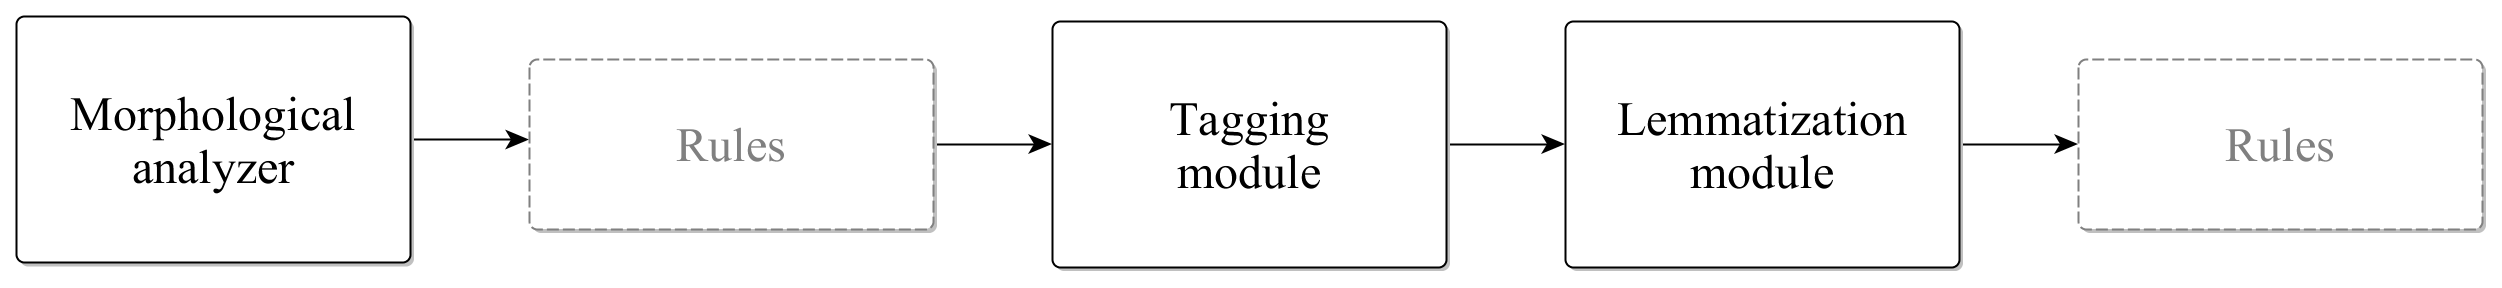
\includegraphics[width=1\textwidth]{MorphTagging/architecture.png} 
  \caption{The architecture of the full morphological tagging tool}
  \label{fig:purepos-arch_en}
\end{figure}

The architecture of PurePos (cf. Figure \ref{fig:purepos-arch_en}) is built up to allow multiple models cooperating effectively. 
The disambiguation is carried out in multiple steps.
The data flow starts from a \acrshort{ma} providing word analyses as \emph{(lemma, tag)} pairs. 
Next, trigram-tagging methods (see \cite{Brants2000,Halacsy2007}) are employed for selecting morphosyntactic labels of words. 
%In fact, these algorithms have been adapted to fit agglutinative languages.
Finally, lemmatization is carried out employing the methods presented in Thesis \ref{thes:morf-lemma}. 

\begin{figure}[H]
  \centering
  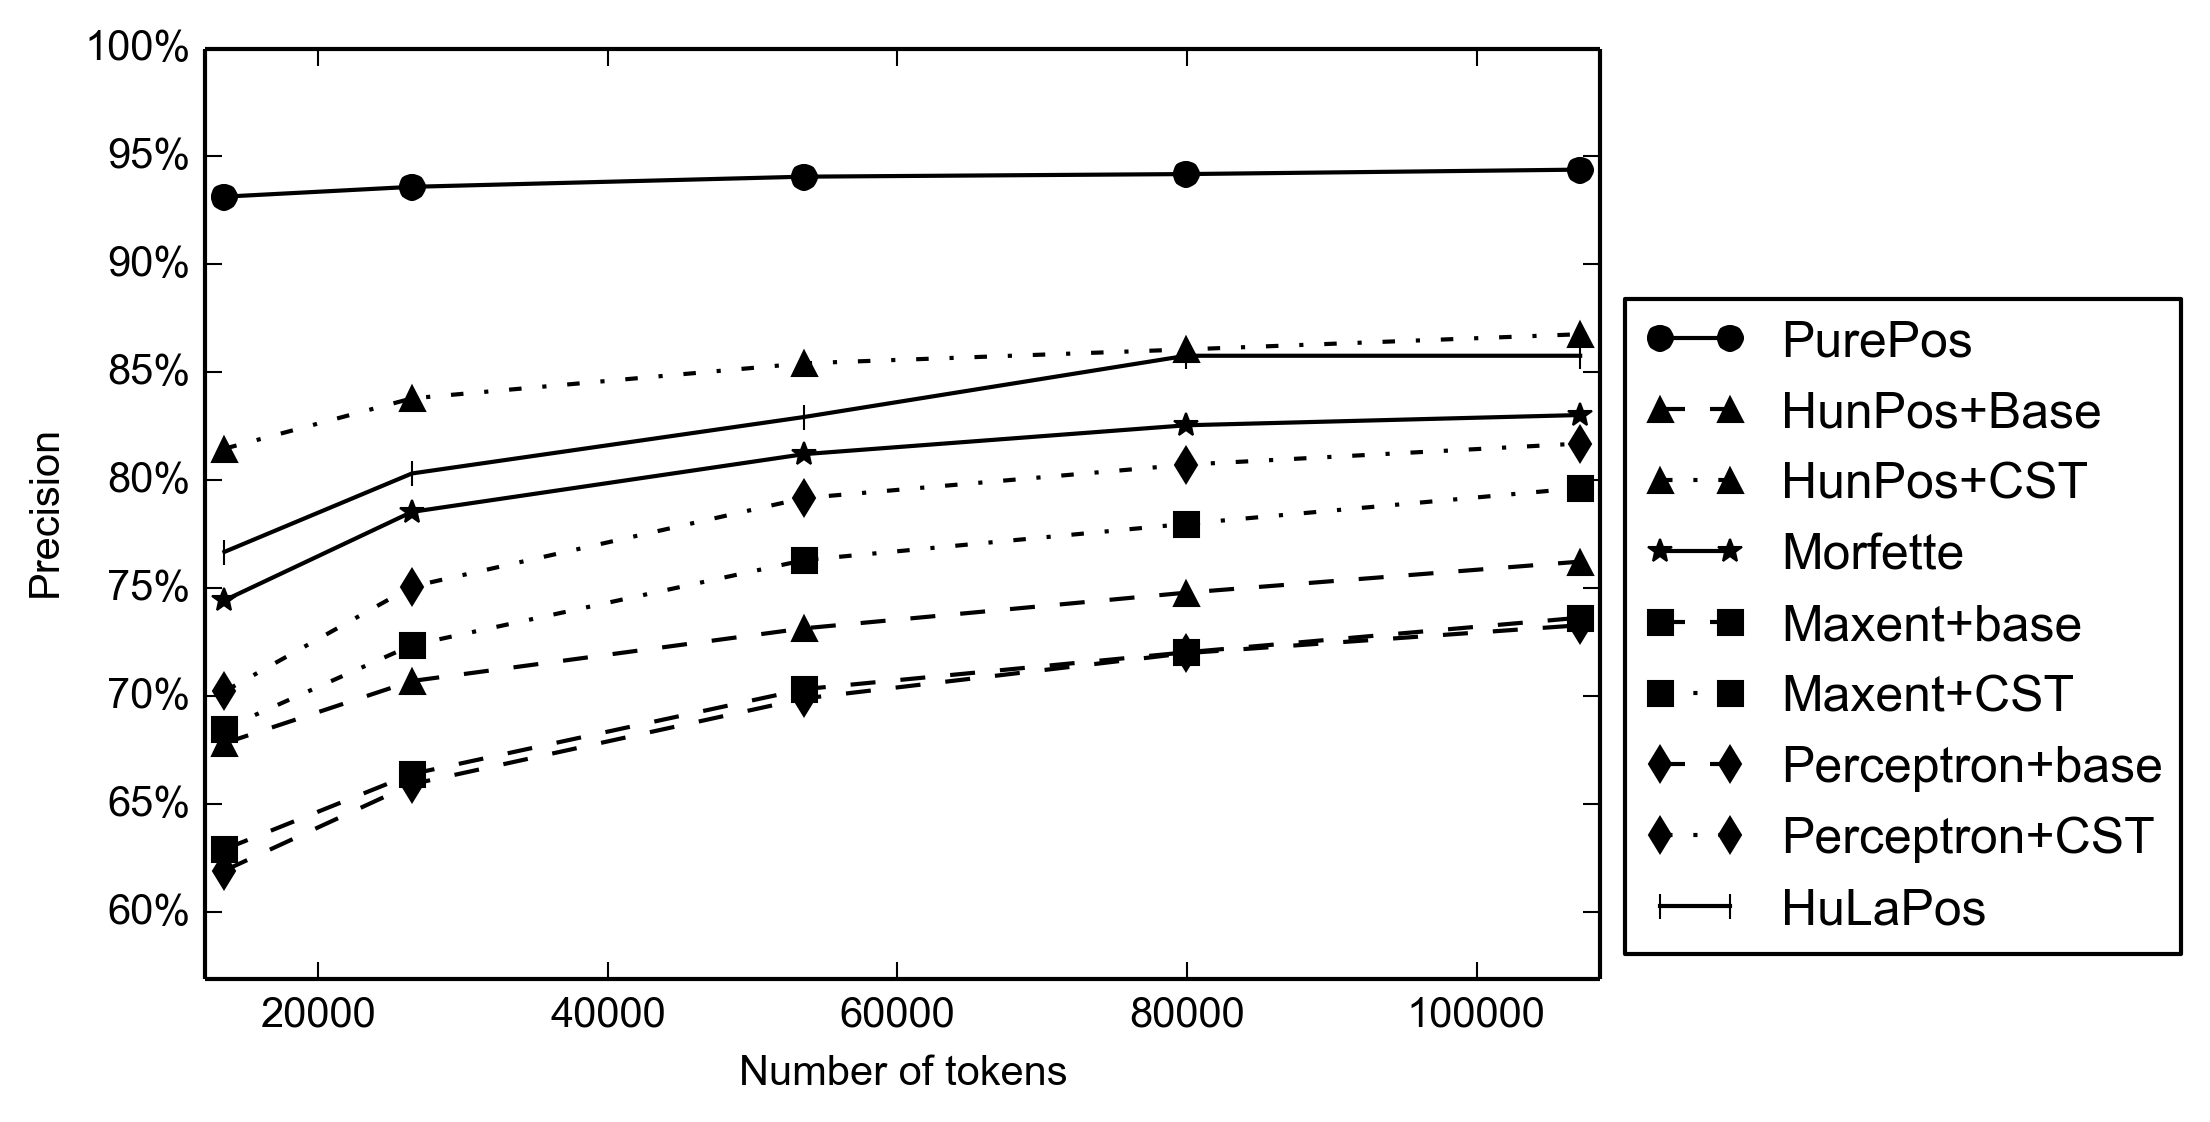
\includegraphics[width=1\textwidth]{MorphTagging/msd_token.png}
  \caption{Learning curves of full morphological taggers on the Szeged Corpus (using Humor labels)}
  \label{fig:humor-token_en}
\end{figure}

Several experiments were carried out measuring the performance of PurePos on the Szeged Corpus \cite{Csendes2004}.
Our results show that the new method yields 96.26\% full tagging accuracy, which is the highest one amongst available tools.
Moving on, we also compared existing tagging systems with ours on a less-resourced scenario.
These experiments showed (cf. Figure \ref{fig:humor-token_en}) that PurePos can be successfully used even when the training dataset is limited.
Finally, all the hybrid enhancements of PurePos ware evaluated one-by-one, showing that they can be used to fix several sorts of errors.


\thesisline%%%%%%%%%%%%%%%%%%%%%%%%%%%%%%%%%%%%%%%%%%%%%%%%%%%%%%%%%%%%%%%%%%%%%

Although, methods of Thesis group \ref{thes:morf-tagging} have high accuracy, we showed that they can be improved further.  
Therefore, a combination technique is presented increasing the ceiling of morphological tagging tools' performance for agglutinative languages.


\begin{core}
\begin{thesis}
We developed a methodology for combining morphological tagging systems effectively.
The system presented selects the best lemma and tag candidates separately using two different combination methods.
These components are trained with cross-validation using instance based learning.
We showed that our method can significantly reduce the number of errors of existing annotation tools.
\end{thesis}

\begin{pub}
\cite{Laki2013a,Orosz2013c,Orosz2013d} 
\end{pub}
\end{core}

First of all, the discrepancy of tagging systems was investigated. 
For this, we designed a new metric (Own Error Rate) which measures the differences of output of taggers.
It turned out that the most typical mistakes of HuLaPos \cite{Laki2013} and PurePos are different enough to be aggregated.

Following this, the most common combination techniques were investigated considering their applicability to full morphological tagging.
Next, a new combination method was presented involving adapted feature sets for morphologically rich languages.
It utilizes instance based learning \cite{Aha1991} and trains classifiers with cross-validation, which
can employ the whole training dataset for both the baseline tools and the level-one learners. %TODO Nóri fordítás
The novelty of the presented method is its architecture (cf. Figure \ref{fig:comb3_en}) allowing us to utilize different combiners for the lemmatization and \acrshort{pos} tagging subtasks.

\begin{figure}[H]
  \centering
  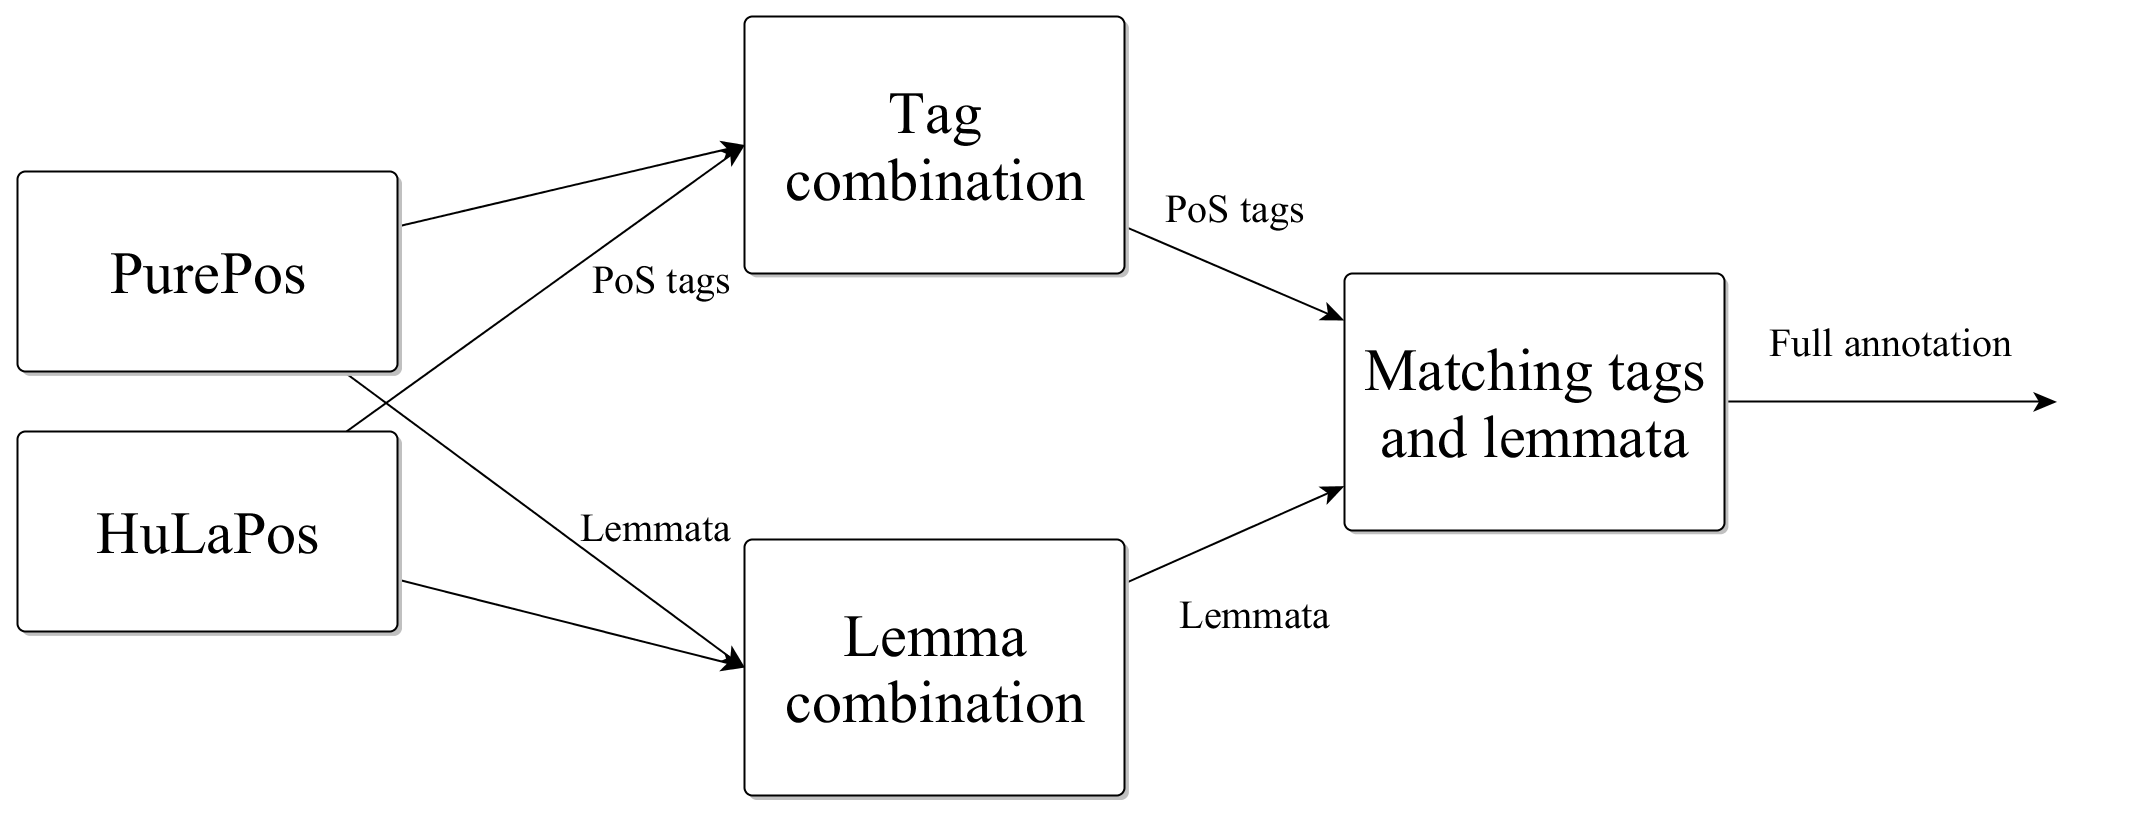
\includegraphics[scale=0.15]{MorphTagging/comb3.png} 
  \caption{Combining the output of two PoS taggers and lemmatizers}
  \label{fig:comb3_en}
\end{figure}

Finally, evaluation experiments were presented indicating that the number errors of the best tagger can be decreased further.
The new algorithm could reduce the number of errors of PurePos by 28.90\%.

\subsection{Measuring morphosyntactic complexity using morphological annotation algorithms}
\label{thes:mlu}


Measuring morphosyntactic complexity is usually carried out calculating \acrlong{mlu}s.
This metric is often computed in words for analytical languages, while morphemes (\acrshort{mlum}) are used for morphologically complex ones.
Although automatic methods and tools exist for e.g English, other less-resourced languages lack such systems.
Therefore, \acrshort{mlum} could be only computed manually, which is a time-consuming task.

This thesis group presents\footnote{This research has been conducted together with Kinga Jelencsik-Mátyus. 
%Manual annotation of the data were performed by both of us, while the morpheme counting principles are her work. 
My contributions are the construction of the tagging chain, its adaptation and the automatization of the MLUm calculation.} methods for processing speech transcripts effectively and estimating \acrlong{mlum} automatically.
%Our solution relies on the PurePos tagger tool (cf. Thesis \ref{thes:morf-tagging}).
%Results also indicate that the labor-intense manual work can be replaced with our new method.


\begin{core}
\begin{thesis}
\label{thes:spoken-morf-tagging}
We developed a hybrid morphological tagging chain for Hungarian child-language transcripts.
Our method builds on top of the results presented in Thesis \ref{thes:morf-tagging} by adapting them to the domain.
Evaluation shows that our performance is comparable with that of tagging methods for written corpora.
Moreover, experiments indicate that the algorithm presented is accurate enough to be used in further applications.
\end{thesis}

\begin{pub}
\cite{Matyus2014,Orosz2014c}
\end{pub}
\end{core}

The proposed method adapts the algorithms introduced in Thesis \ref{thes:morf-tagging} for spoken Hungarian.
For this, the Humor \acrlong{ma} was augmented first with analyses of words typical to the domain.
Next, the output of PurePos was adjusted utilizing domain-specific knowledge.

For this, a gold corpus of about 1,000 utterances from the \acrshort{hukilc} was created by the manual annotation of texts. 
Additionally, a new tagging scheme was designed representing the characteristics of spoken language properly.
%These manually corrected texts enabled us to develop and validate the proposed methods.

The evaluation of the chain resulted in 96\% token-level precision, which is comparable with that of taggers for corpora of written language.
Therefore, our investigation showed the PurePos is an appropriate base for tagging corpora of transcribed spoken texts.

\thesisline%%%%%%%%%%%%%%%%%%%%%%%%%%%%%%%%%%%%%%%%%%%%%%%%%%%%%%%%%%%%%%%%%%%%%


\begin{core}
\begin{thesis}
\label{thes:mlu-estimation}
We proposed a new algorithm for estimating morphosyntactic complexity (calculating \acrlong{mlum}) in Hungarian child language transcripts.
The method uses the morphological tagging chain of Thesis \ref{thes:spoken-morf-tagging} as a base.
%In doing so, it computes lengths of utterances in its output.
Evaluation of the system indicates that our methodology can properly replace the time-consuming manual computation of human annotators.
\end{thesis}

\begin{pub}
\cite{Matyus2014,Orosz2014c}
\end{pub}
\end{core}

The estimation method analyzes morphological annotation of tokens.
Words known by the analyzer are decomposed by Humor, while lengths of unknown words are guessed based on their \acrshort{pos} labels.
This is followed by morpheme counting rules implementing linguistic guidelines, thus providing relevant estimates.

As regards resources, a manually checked corpus was created for the experiments.
Evaluation of the methods on this dataset shows that our results highly correlate (0.9901) with counts of human annotators.
Further on, we showed that the mean relative error of the method is only 4.49\%.
Thus, the proposed algorithm can properly replace the labor-intensive human computation.

\subsection{Effective preprocessing methods for a less-resourced noisy domain}
\label{thes:clin}

More and more electronic health records are produced in hospitals containing valuable but hidden knowledge.
Since doctors cannot spend enough time on writing their reports properly, notes often contain numerous errors.
Because of such mistakes, processing of these reports cannot be carried out using general-purpose tools.
Moreover, while several algorithms are becoming available for English, Hungarian and other morphologically rich languages are still neglected.

\begin{core}
\begin{thesis}%{II.1/b}
\label{thes:clin-segment}
We developed a new framework which segments noisy clinical records into words and sentences accurately.
The method is built on top of well-known tokenization rules (e.g. \cite{Halacsy2004}), however, it augments them with unsupervised heuristics.
Our evaluation showed that the tool can properly identify word and sentence boundaries in noisy clinical notes. 
Results also indicate that other systems available cannot handle such erroneous texts.
\end{thesis}

\begin{pub}
\cite{Orosz2013d,Orosz2014a,Orosz2014x}
\end{pub}
\end{core}

\begin{figure}[H]
  \centering
  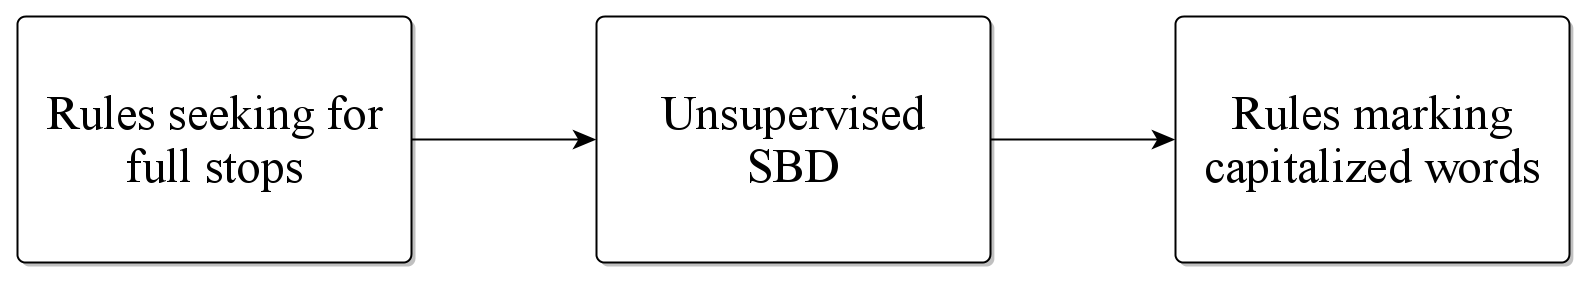
\includegraphics[scale=0.2]{Clinical/clin_segm_arch.png} 
  \caption{The architecture of the proposed method}
  \label{fig:clin-segment-arch_en}
\end{figure}

The proposed method builds on pattern-matching algorithms taken from general-purpose tokenization tools.
Even though these methods perform with high accuracy, their recall still stays low.
Therefore, this study proposes a method (see Figure \ref{fig:clin-segment-arch_en}) which improves their performance using unsupervised heuristics and a domain-specific morphologic analyzer.
First, the scaled $\log\lambda$  method \cite{kiss2006unsupervised} was adapted by introducing new factors.
Next, the Humor morphological analyzer was utilized to reveal further sentence boundaries.

The evaluation of the framework was carried out on a manually segmented corpus. 
Numerous metrics (such as precision, recall, F-score) were employed measuring the performance of the proposed tool.
Thus, we could analyze both the tokenization and the sentence boundary detection accuracy of the tool.
Besides, existing Hungarian approaches were also compared with the proposed one.

Results show that systems available can only produce low quality segmentation.
Moreover, most of them result in F-scores less than 50\% in sentence boundary identification.
On the contrary, our method can detect both token and sentence boundaries accurately, producing F-values over 90\%.


%%%%%%%%%%%%%%%%%%%%%%%
\thesisline%%%%%%%%%%%%
%%%%%%%%%%%%%%%%%%%%%%%

\begin{core}
\begin{thesis}%{II.2}
\label{thes:clin-pos}
We showed that tagging the methods of Thesis \ref{thes:morf-tagging} can be modified for annotating electronic health records satisfactorily.
For the task, PurePos was adjusted with stochastic and symbolic domain adaptation techniques.
The quality of the annotation produced is comparable with that of general written tagger tools.
\end{thesis}

\begin{pub}
\cite{Orosz2013,Orosz2014b,Orosz2014x} 
\end{pub}
\end{core}

First of all, an extended version of the Humor analyzer was used as a base of the tagging chain, since it was prepared\footnote{The lexicon extension was carried out by Attila Novák \cite{Orosz2014} .} for electronic health records.
Further on, the tagging chain was improved using a detailed error analysis of the baseline tagger.

For this, a manually annotated corpus was created containing texts of clinical notes.
Results on this dataset show that the improved system performs significantly better (93.73\%) than the baseline system (88.09\%).
However, future work might target the segmentation and tagging tasks with a unified framework, since both systems have the most problems with abbreviated terms.

\let\thesubsection=\oldthesubsection

% \pagebreak
\section{Applications}

Methods presented solve basic preprocessing tasks such as text segmentation and morphological tagging. 
Since these are essential components of any language processing chain, our results can be applied in numerous fields of natural language technology. 
In general, text mining solutions and information extraction methods utilize such algorithms.
%Specific applications can employ them  in e.g. named entities recognition, keyword extraction or event identification scenarios. 
Since our results aim morphologically rich and less-resourced languages, they can effectively boost task involving such languages.

Concerning general tagging methods of Theses \ref{thes:morf-lemma} and \ref{thes:morf-tagging}, they have been successfully applied in several Hungarian projects.
Applications are the following:
\begin{enumerate}
\item Laki et al. \cite{Laki2013} have developed an English to Hungarian morpheme-based statistical machine translation method using PurePos,
\item Novák et al. \cite{Novak2013} have annotated Old and Middle Hungarian employing our methods,
\item Enrédy et al. \cite{Endredy2014} have proposed a noun phrase detection toolkit utilizing the morphological tagging tool presented,
\item Indig and Prószéky have applied \cite{Indig2013} the proposed tagger tool for a batch spelling-correction tool and
\item Prószéky et al. \cite{Proszeky2014} have builded their psycho-linguistically motivated parsed on top of PurePos.
\end{enumerate}

Next, Thesis group \ref{thes:mlu} presents methods and resources for analyzing spoken language which can serve \acrshort{nlp} applications of the domain.
Besides, methods of Thesis \ref{thes:mlu-estimation} estimate morphosyntactic-complexity of children language, thus can replace the labor-intense manual work.
Furthermore, Mátyus utilizes \cite{Matyus2014b} these algorithms in her research investigating the speech of Hungarian kindergarten children.

Finally, the last (\ref{thes:clin}) Thesis group details methods for processing noisy texts effectively.
Algorithms of Thesis \ref{thes:clin-segment} segments clinical texts accurately, providing proper output for information extraction applications. 
Furthermore, lessons learned from our tagging methods could help to develop more accurate annotation tools.
Beside possible applications, an ongoing project \cite{Siklosi2014,Siklosi2014mszny} processing Hungarian electronic health records benefits from the proposed methods.


 


\chapter*{Bibliography}
\phantomsection

\addcontentsline{toc}{chapter}{Bibliography}

\addcontentsline{toc}{section}{The author's publications}
\printbibliography[heading=subbibliography,title={The author`s journal publications}, keyword=own, type=article]

\printbibliography[heading=subbibliography,title={The author`s book section publications}, keyword=own, type=incollection]

\printbibliography[heading=subbibliography,title={The author's international conference publications}, keyword=own,notkeyword=hun-conf,type=inproceedings]

\printbibliography[heading=subbibliography,title={The author's other conference publications}, keyword=own, keyword=hun-conf]

\addcontentsline{toc}{section}{References}
\printbibliography[heading=subbibliography,title={References}, notkeyword=own]



% ********************************** Bibliography ******************************





\end{document}
